\days{7 marzo 2023}
\paragrafo{Esempio}{%
\[
    \begin{cases}
        x'=y^{2}-xy^{2}\\ 
        y'=-x\,y^{3}
    \end{cases}\qquad \begin{aligned}
    \bm{f}: \R^{2} &\longrightarrow \R^{2} \\
    (x,y) &\longmapsto (y^{2}-xy^{2}, -xy^{3})
    \end{aligned}
\]\begin{enumerate}
    \item \emph{Equilibri}: \[
        \begin{cases}
            y^{2}(1-x)=0\\ 
            x\,y^{3} = 0
        \end{cases}
    \]la prima equazione è soddisfatta per $ x = 1 \vee y = 0 $, mentre la seconda è soddisfatta per $ x = 0 \vee  y = 0 $. Quindi:
        \begin{align*}
            f(x,y)=\bm{0} \iff y=0
        \end{align*}
    $\Rightarrow$ $ \displaystyle \left\{(x,0): x \in \R\right\} $ è composto da equilibri. 
    \item \emph{Punti con tangente verticale} [$ x'=0 $]:
    
     Oltre ai punti di equilibrio, sono tutti i punti sulla retta verticale $ x=1 $. Questa quindi è una retta invariante, composta da orbite.

    Se $ x = 1 $ abbiamo \[
        \begin{cases}
            x'=0\\ 
            y'=-y^{3}
        \end{cases}
    \]
    \item \emph{Punti con tangente orizzontale} [$ y'=0 $]: 
    
    Oltre ai punti di equilibrio, sono tutti i punti sulla retta verticale $ x=0 $.

    Se $ x=0 $ abbiamo \[
        \begin{cases}
            x'=y^{2}>0\\ 
            y'=0
        \end{cases}
    \]
    \begin{figure}[H]
        \begin{center}
            \begin{tikzpicture}
                \draw [-Latex] (-3,0) -- (3,0);
                \draw [-Latex] (0,-3) -- (0,3);
                \node at (3,-0.2) {$x$};
                \node at (-0.2,3) {$y$};
                \foreach \i in{-2.4,-2,...,2.4}{
                    \fill (0,\i) circle (0.05);
                    \draw [-Latex, thin] (0,\i) -- (0.4,\i);
                };
                \draw [thick,-Latex] (1,3) -- (1,1.3);
                \draw [thick] (1,1.5) -- (1,-1.5);
                \draw [thick,-Latex] (1,-3) -- (1,-1.3);
                \fill (1,0) circle (0.1);
            \end{tikzpicture}
        \end{center}
        \caption{Punti con tangenti verticali e orizzontali per l'esempio \framref{dafasdflkjnsadfkjnasdfkjnadskfjnasdkfjnldskjn}}
    \end{figure}
    \item \emph{Equazioni delle orbite}: per $ y\neq 0 $ e $ x\neq 1 $ abbiamo: \begin{equation}
        \frac{d\,y}{dx} =\frac{-xy^{3}}{y^{2}(1-x)}\quad\leadsto\quad \begin{cases}
            y'(x)=\displaystyle\frac{-x}{1-x}\,y(x) \label{eq:diff:orb}\\ 
            y(x_0)=y_0
        \end{cases}
    \end{equation}e integrando si ottiene \[
        \ln\frac{|y|}{|y_0|} = x-x_0 + \ln\frac{|x-1|}{|x_0-1|}
    \]Notiamo che, poiché le orbite non intersecano l'asse $ x $ (poiché sono altre orbite), $ y(x) $ e $ y_0 $ hanno lo stesso segno, dunque posso ``eliminare'' i valori assoluti. Con lo stesso ragionamento è lecito ``eliminare'' anche il secondo valore assoluto. Cosi facendo abbiamo: \[
        \ln\frac{y}{y_0} = x-x_0 + \ln\frac{x-1}{x_0-1}
    \]Facendo l'esponenziale da ambo le parti otteniamo \[
        y(x)= y_0\,\frac{x-1}{x_0-1}\,e^{x-x_0}
    \]Alcune osservazioni: \begin{enumerate}
        \item Le orbite con dato iniziale $ (x_0,y_0) $ e $ (x_0,-y_0) $ sono simmetriche rispetto all'asse orizzontale 
        
        $\implies$ consideriamo solo $ y_0 >0$. 

        Dividiamo ancora i due casi: \begin{itemize}
            \item $ x_0>1 $ $ \,\implies\, $ $ \displaystyle y_0\,\frac{x-1}{x_0-1}>0 $\[
                \,\implies\,\lim_{x\to 1^{+}} y(x) = 0^{+},\qquad \lim_{x\to + \infty} y(x) = + \infty
            \]e guardando l'equazione differenziale delle orbite \eqref{eq:diff:orb}\[
                y'(x)=\frac{x}{x-1}\,y(x) >0
            \]e quindi $ y $ come funzione di $ x $ è monotona crescente.
            
            Notiamo inoltre che per $ x_0>1 $, $ x'=y^{2}(1-x)<0 $, dunque le frecce delle orbite sono rivolte verso $ x=1 $. 
            \item $ x_0<1 $ $ \,\implies\, $ $ \displaystyle \frac{y_0}{x_0-1}>0 $, $ x-1<0 $: \[
                \lim_{x\to 1^{-}} y(x) = 0^{+},\qquad \lim_{x\to - \infty} y(x) = 0^{+}
            \]e inoltre la funzione è sempre positiva. 

            Poichè $ x'>0 \leadsto$ le frecce sono rivolte verso $ x=1$ (vedi \ref{fig:orbitedivattelaapesce}).
        \end{itemize}
        \begin{figure}[H]
            \begin{center}
                % This file was created by matlab2tikz.
%
%The latest updates can be retrieved from
%  http://www.mathworks.com/matlabcentral/fileexchange/22022-matlab2tikz-matlab2tikz
%where you can also make suggestions and rate matlab2tikz.
%
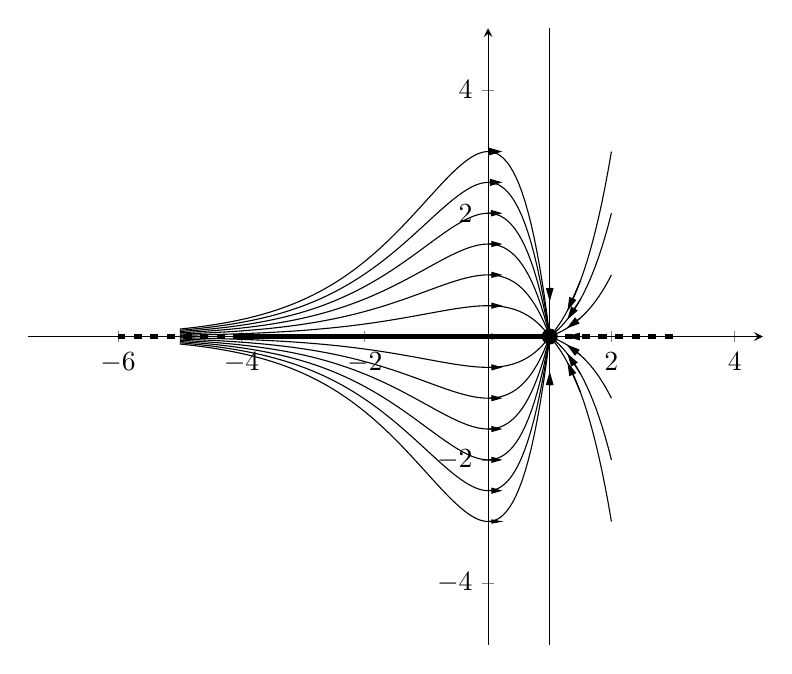
\begin{tikzpicture}


  \begin{axis}[%
    width=0.9*\textwidth,
    axis equal,
    axis lines=middle,
    xmin=-4,
    xmax=1,
    ymin=-5,
    ymax=5,
    axis background/.style={fill=white}
    ]
    \draw (1,5) -- (1,-5);
    \draw [ultra thick] (-4,0) -- (1,0);
    \draw [ultra thick, dashed] (-4,0) -- (-6,0);
    \draw [ultra thick, dashed] (3,0) -- (1,0);
    \fill (1,0) circle (0.13);
\addplot [color=black, forget plot]
  table[row sep=crcr]{%
-5	-0.121283045983538\\
-4.95	-0.12643884938358\\
-4.9	-0.131804520355361\\
-4.85	-0.137388025988912\\
-4.8	-0.143197598652949\\
-4.75	-0.149241742253831\\
-4.7	-0.155529238438998\\
-4.65	-0.162069152722712\\
-4.6	-0.168870840509844\\
-4.55	-0.175943952991147\\
-4.5	-0.183298442880998\\
-4.45	-0.190944569965966\\
-4.4	-0.198892906429709\\
-4.35	-0.207154341916702\\
-4.3	-0.215740088293995\\
-4.25	-0.224661684066738\\
-4.2	-0.233930998399452\\
-4.15	-0.243560234691002\\
-4.1	-0.253561933646947\\
-4.05	-0.263948975788327\\
-4	-0.274734583331013\\
-3.95	-0.285932321364496\\
-3.9	-0.297556098253325\\
-3.85	-0.309620165178388\\
-3.8	-0.322139114728785\\
-3.75	-0.33512787844813\\
-3.7	-0.348601723231785\\
-3.65	-0.362576246463637\\
-3.6	-0.377067369772637\\
-3.55	-0.392091331280368\\
-3.5	-0.4076646762013\\
-3.45	-0.423804245647207\\
-3.4	-0.440527163476304\\
-3.35	-0.457850821016028\\
-3.3	-0.475792859475996\\
-3.25	-0.494371149854456\\
-3.2	-0.513603770127414\\
-3.15	-0.53350897949465\\
-3.1	-0.554105189440761\\
-3.05	-0.575410931352362\\
-3	-0.597444820414367\\
-2.95	-0.620225515488924\\
-2.9	-0.643771674659965\\
-2.85	-0.668101906104384\\
-2.8	-0.693234713927485\\
-2.75	-0.71918843857546\\
-2.7	-0.745981191411223\\
-2.65	-0.773630783011704\\
-2.6	-0.802154644714806\\
-2.55	-0.831569742912281\\
-2.5	-0.861892485550937\\
-2.45	-0.893138620268485\\
-2.4	-0.925323123552008\\
-2.35	-0.958460080266274\\
-2.3	-0.992562552855757\\
-2.25	-1.02764243947818\\
-2.2	-1.06371032027841\\
-2.15	-1.10077529095955\\
-2.1	-1.13884478275273\\
-2.05	-1.17792436782841\\
-2	-1.21801754912951\\
-1.95	-1.25912553354065\\
-1.9	-1.30124698723692\\
-1.85	-1.34437777198152\\
-1.8	-1.38851066106133\\
-1.75	-1.43363503346617\\
-1.7	-1.47973654482715\\
-1.65	-1.52679677353499\\
-1.6	-1.57479284035831\\
-1.55	-1.62369699977458\\
-1.5	-1.67347620111322\\
-1.45	-1.72409161748941\\
-1.4	-1.77549814037957\\
-1.35	-1.82764383755354\\
-1.3	-1.88046937193469\\
-1.25	-1.93390737880628\\
-1.2	-1.98788179862053\\
-1.15	-2.04230716249489\\
-1.1	-2.0970878272979\\
-1.05	-2.1521171570336\\
-1	-2.20727664702865\\
-0.95	-2.26243498720883\\
-0.9	-2.31744706052141\\
-0.85	-2.37215287231543\\
-0.8	-2.426376406233\\
-0.75	-2.47992440189033\\
-0.7	-2.53258504933619\\
-0.65	-2.58412659496703\\
-0.6	-2.63429585325133\\
-0.55	-2.68281661826926\\
-0.5	-2.72938796870685\\
-0.45	-2.77368245955471\\
-0.4	-2.81534419334968\\
-0.35	-2.85398676336079\\
-0.3	-2.8891910606587\\
-0.25	-2.92050293651777\\
-0.2	-2.94743071108073\\
-0.15	-2.96944251866645\\
-0.1	-2.98596347951867\\
-0.05	-2.99637268717725\\
0	-3\\
0.0499999999999999	-2.99612262467167\\
0.1	-2.98396147880425\\
0.15	-2.96267731895712\\
0.2	-2.93136661958441\\
0.25	-2.88905718754742\\
0.3	-2.83470349590961\\
0.35	-2.76718171975685\\
0.4	-2.68528445575429\\
0.45	-2.58771510605878\\
0.5	-2.47308190605019\\
0.55	-2.33989157412098\\
0.6	-2.18654256046861\\
0.65	-2.01131787046459\\
0.7	-1.81237743672343\\
0.75	-1.58775001245951\\
0.8	-1.33532455709548\\
0.85	-1.0528410833667\\
0.9	-0.737880933347085\\
0.95	-0.387856448897377\\
1	0\\
};

\addplot[area legend, draw=black, fill=black, forget plot]
table[row sep=crcr] {%
x	y\\
0.0308755760368662	-3\\
0	-3\\
0	-3\\
0	-3\\
0	-3\\
0	-3\\
0.0617511520737324	-3\\
0.0617511520737324	-3.02513105922514\\
0.2	-3\\
0.0617511520737324	-2.97486894077486\\
0.0617511520737324	-3\\
}--cycle;
\addplot [color=black, forget plot]
  table[row sep=crcr]{%
-5	-0.101069204986282\\
-4.95	-0.10536570781965\\
-4.9	-0.109837100296134\\
-4.85	-0.114490021657427\\
-4.8	-0.11933133221079\\
-4.75	-0.124368118544859\\
-4.7	-0.129607698699165\\
-4.65	-0.135057627268927\\
-4.6	-0.14072570042487\\
-4.55	-0.146619960825956\\
-4.5	-0.152748702400832\\
-4.45	-0.159120474971638\\
-4.4	-0.165744088691424\\
-4.35	-0.172628618263918\\
-4.3	-0.179783406911662\\
-4.25	-0.187218070055615\\
-4.2	-0.19494249866621\\
-4.15	-0.202966862242502\\
-4.1	-0.211301611372456\\
-4.05	-0.219957479823606\\
-4	-0.228945486109177\\
-3.95	-0.238276934470413\\
-3.9	-0.247963415211104\\
-3.85	-0.258016804315323\\
-3.8	-0.268449262273987\\
-3.75	-0.279273232040108\\
-3.7	-0.290501436026488\\
-3.65	-0.302146872053031\\
-3.6	-0.314222808143865\\
-3.55	-0.326742776066974\\
-3.5	-0.339720563501083\\
-3.45	-0.353170204706006\\
-3.4	-0.367105969563587\\
-3.35	-0.38154235084669\\
-3.3	-0.39649404956333\\
-3.25	-0.411975958212046\\
-3.2	-0.428003141772845\\
-3.15	-0.444590816245542\\
-3.1	-0.461754324533968\\
-3.05	-0.479509109460302\\
-3	-0.497870683678639\\
-2.95	-0.51685459624077\\
-2.9	-0.536476395549971\\
-2.85	-0.55675158842032\\
-2.8	-0.577695594939571\\
-2.75	-0.599323698812883\\
-2.7	-0.621650992842686\\
-2.65	-0.64469231917642\\
-2.6	-0.668462203929005\\
-2.55	-0.692974785760234\\
-2.5	-0.718243737959114\\
-2.45	-0.744282183557071\\
-2.4	-0.771102602960006\\
-2.35	-0.798716733555228\\
-2.3	-0.827135460713131\\
-2.25	-0.856368699565148\\
-2.2	-0.886425266898671\\
-2.15	-0.917312742466289\\
-2.1	-0.94903731896061\\
-2.05	-0.981603639857007\\
-2	-1.0150146242746\\
-1.95	-1.04927127795054\\
-1.9	-1.0843724893641\\
-1.85	-1.1203148099846\\
-1.8	-1.15709221755111\\
-1.75	-1.19469586122181\\
-1.7	-1.23311378735596\\
-1.65	-1.2723306446125\\
-1.6	-1.31232736696526\\
-1.55	-1.35308083314549\\
-1.5	-1.39456350092769\\
-1.45	-1.43674301457451\\
-1.4	-1.47958178364964\\
-1.35	-1.52303653129461\\
-1.3	-1.56705780994557\\
-1.25	-1.61158948233857\\
-1.2	-1.65656816551711\\
-1.15	-1.70192263541241\\
-1.1	-1.74757318941492\\
-1.05	-1.79343096419467\\
-1	-1.83939720585721\\
-0.95	-1.88536248934069\\
-0.9	-1.93120588376785\\
-0.85	-1.97679406026286\\
-0.8	-2.0219803385275\\
-0.75	-2.06660366824194\\
-0.7	-2.11048754111349\\
-0.65	-2.15343882913919\\
-0.6	-2.19524654437611\\
-0.55	-2.23568051522439\\
-0.5	-2.27448997392238\\
-0.45	-2.31140204962893\\
-0.4	-2.34612016112474\\
-0.35	-2.37832230280066\\
-0.3	-2.40765921721558\\
-0.25	-2.43375244709814\\
-0.2	-2.45619225923395\\
-0.15	-2.47453543222204\\
-0.1	-2.48830289959889\\
-0.05	-2.49697723931437\\
0	-2.5\\
0.0499999999999999	-2.49676885389306\\
0.1	-2.48663456567021\\
0.15	-2.4688977657976\\
0.2	-2.44280551632034\\
0.25	-2.40754765628952\\
0.3	-2.36225291325801\\
0.35	-2.30598476646404\\
0.4	-2.23773704646191\\
0.45	-2.15642925504898\\
0.5	-2.06090158837516\\
0.55	-1.94990964510082\\
0.6	-1.82211880039051\\
0.65	-1.67609822538716\\
0.7	-1.51031453060286\\
0.75	-1.32312501038292\\
0.8	-1.11277046424623\\
0.85	-0.877367569472247\\
0.9	-0.614900777789237\\
0.95	-0.323213707414481\\
1	0\\
};

\addplot[area legend, draw=black, fill=black, forget plot]
table[row sep=crcr] {%
x	y\\
0.0308755760368662	-2.5\\
0	-2.5\\
0	-2.5\\
0	-2.5\\
0	-2.5\\
0	-2.5\\
0.0617511520737324	-2.5\\
0.0617511520737324	-2.53964221922933\\
0.2	-2.5\\
0.0617511520737324	-2.46035778077067\\
0.0617511520737324	-2.5\\
}--cycle;
\addplot [color=black, forget plot]
  table[row sep=crcr]{%
-5	-0.0808553639890256\\
-4.95	-0.0842925662557202\\
-4.9	-0.0878696802369072\\
-4.85	-0.0915920173259415\\
-4.8	-0.0954650657686323\\
-4.75	-0.0994944948358873\\
-4.7	-0.103686158959332\\
-4.65	-0.108046101815142\\
-4.6	-0.112580560339896\\
-4.55	-0.117295968660764\\
-4.5	-0.122198961920665\\
-4.45	-0.12729637997731\\
-4.4	-0.132595270953139\\
-4.35	-0.138102894611135\\
-4.3	-0.14382672552933\\
-4.25	-0.149774456044492\\
-4.2	-0.155953998932968\\
-4.15	-0.162373489794001\\
-4.1	-0.169041289097965\\
-4.05	-0.175965983858884\\
-4	-0.183156388887342\\
-3.95	-0.190621547576331\\
-3.9	-0.198370732168883\\
-3.85	-0.206413443452259\\
-3.8	-0.21475940981919\\
-3.75	-0.223418585632087\\
-3.7	-0.23240114882119\\
-3.65	-0.241717497642425\\
-3.6	-0.251378246515092\\
-3.55	-0.261394220853579\\
-3.5	-0.271776450800866\\
-3.45	-0.282536163764805\\
-3.4	-0.29368477565087\\
-3.35	-0.305233880677352\\
-3.3	-0.317195239650664\\
-3.25	-0.329580766569637\\
-3.2	-0.342402513418276\\
-3.15	-0.355672652996434\\
-3.1	-0.369403459627174\\
-3.05	-0.383607287568242\\
-3	-0.398296546942912\\
-2.95	-0.413483676992616\\
-2.9	-0.429181116439976\\
-2.85	-0.445401270736256\\
-2.8	-0.462156475951657\\
-2.75	-0.479458959050307\\
-2.7	-0.497320794274148\\
-2.65	-0.515753855341136\\
-2.6	-0.534769763143204\\
-2.55	-0.554379828608187\\
-2.5	-0.574594990367292\\
-2.45	-0.595425746845657\\
-2.4	-0.616882082368005\\
-2.35	-0.638973386844183\\
-2.3	-0.661708368570505\\
-2.25	-0.685094959652118\\
-2.2	-0.709140213518937\\
-2.15	-0.733850193973031\\
-2.1	-0.759229855168488\\
-2.05	-0.785282911885606\\
-2	-0.812011699419676\\
-1.95	-0.83941702236043\\
-1.9	-0.867497991491283\\
-1.85	-0.896251847987677\\
-1.8	-0.925673774040884\\
-1.75	-0.955756688977448\\
-1.7	-0.986491029884767\\
-1.65	-1.01786451569\\
-1.6	-1.04986189357221\\
-1.55	-1.08246466651639\\
-1.5	-1.11565080074215\\
-1.45	-1.14939441165961\\
-1.4	-1.18366542691971\\
-1.35	-1.21842922503569\\
-1.3	-1.25364624795646\\
-1.25	-1.28927158587086\\
-1.2	-1.32525453241369\\
-1.15	-1.36153810832993\\
-1.1	-1.39805855153193\\
-1.05	-1.43474477135574\\
-1	-1.47151776468577\\
-0.95	-1.50828999147255\\
-0.9	-1.54496470701428\\
-0.85	-1.58143524821029\\
-0.8	-1.617584270822\\
-0.75	-1.65328293459355\\
-0.7	-1.68839003289079\\
-0.65	-1.72275106331135\\
-0.6	-1.75619723550088\\
-0.55	-1.78854441217951\\
-0.5	-1.8195919791379\\
-0.45	-1.84912163970314\\
-0.4	-1.87689612889979\\
-0.35	-1.90265784224053\\
-0.3	-1.92612737377247\\
-0.25	-1.94700195767851\\
-0.2	-1.96495380738716\\
-0.15	-1.97962834577763\\
-0.1	-1.99064231967911\\
-0.05	-1.9975817914515\\
0	-2\\
0.0499999999999999	-1.99741508311445\\
0.1	-1.98930765253617\\
0.15	-1.97511821263808\\
0.2	-1.95424441305627\\
0.25	-1.92603812503161\\
0.3	-1.8898023306064\\
0.35	-1.84478781317123\\
0.4	-1.79018963716952\\
0.45	-1.72514340403919\\
0.5	-1.64872127070013\\
0.55	-1.55992771608066\\
0.6	-1.45769504031241\\
0.65	-1.34087858030973\\
0.7	-1.20825162448229\\
0.75	-1.05850000830634\\
0.8	-0.890216371396987\\
0.85	-0.701894055577797\\
0.9	-0.49192062223139\\
0.95	-0.258570965931585\\
1	0\\
};

\addplot[area legend, draw=black, fill=black, forget plot]
table[row sep=crcr] {%
x	y\\
0.0308755760368662	-2\\
0	-2\\
0	-2\\
0	-2\\
0	-2\\
0	-2\\
0.0617511520737324	-2\\
0.0617511520737324	-2.03964221922933\\
0.2	-2\\
0.0617511520737324	-1.96035778077067\\
0.0617511520737324	-2\\
}--cycle;
\addplot [color=black, forget plot]
  table[row sep=crcr]{%
-5	-0.0606415229917692\\
-4.95	-0.0632194246917902\\
-4.9	-0.0659022601776804\\
-4.85	-0.0686940129944562\\
-4.8	-0.0715987993264743\\
-4.75	-0.0746208711269155\\
-4.7	-0.0777646192194992\\
-4.65	-0.0810345763613562\\
-4.6	-0.0844354202549221\\
-4.55	-0.0879719764955733\\
-4.5	-0.091649221440499\\
-4.45	-0.0954722849829828\\
-4.4	-0.0994464532148544\\
-4.35	-0.103577170958351\\
-4.3	-0.107870044146997\\
-4.25	-0.112330842033369\\
-4.2	-0.116965499199726\\
-4.15	-0.121780117345501\\
-4.1	-0.126780966823474\\
-4.05	-0.131974487894163\\
-4	-0.137367291665506\\
-3.95	-0.142966160682248\\
-3.9	-0.148778049126662\\
-3.85	-0.154810082589194\\
-3.8	-0.161069557364392\\
-3.75	-0.167563939224065\\
-3.7	-0.174300861615893\\
-3.65	-0.181288123231819\\
-3.6	-0.188533684886319\\
-3.55	-0.196045665640184\\
-3.5	-0.20383233810065\\
-3.45	-0.211902122823604\\
-3.4	-0.220263581738152\\
-3.35	-0.228925410508014\\
-3.3	-0.237896429737998\\
-3.25	-0.247185574927228\\
-3.2	-0.256801885063707\\
-3.15	-0.266754489747325\\
-3.1	-0.277052594720381\\
-3.05	-0.287705465676181\\
-3	-0.298722410207184\\
-2.95	-0.310112757744462\\
-2.9	-0.321885837329982\\
-2.85	-0.334050953052192\\
-2.8	-0.346617356963742\\
-2.75	-0.35959421928773\\
-2.7	-0.372990595705611\\
-2.65	-0.386815391505852\\
-2.6	-0.401077322357403\\
-2.55	-0.415784871456141\\
-2.5	-0.430946242775469\\
-2.45	-0.446569310134243\\
-2.4	-0.462661561776004\\
-2.35	-0.479230040133137\\
-2.3	-0.496281276427879\\
-2.25	-0.513821219739089\\
-2.2	-0.531855160139203\\
-2.15	-0.550387645479773\\
-2.1	-0.569422391376366\\
-2.05	-0.588962183914204\\
-2	-0.609008774564757\\
-1.95	-0.629562766770323\\
-1.9	-0.650623493618462\\
-1.85	-0.672188885990758\\
-1.8	-0.694255330530663\\
-1.75	-0.716817516733086\\
-1.7	-0.739868272413575\\
-1.65	-0.763398386767497\\
-1.6	-0.787396420179156\\
-1.55	-0.811848499887292\\
-1.5	-0.836738100556612\\
-1.45	-0.862045808744706\\
-1.4	-0.887749070189783\\
-1.35	-0.913821918776768\\
-1.3	-0.940234685967343\\
-1.25	-0.966953689403142\\
-1.2	-0.993940899310267\\
-1.15	-1.02115358124745\\
-1.1	-1.04854391364895\\
-1.05	-1.0760585785168\\
-1	-1.10363832351433\\
-0.95	-1.13121749360442\\
-0.9	-1.15872353026071\\
-0.85	-1.18607643615772\\
-0.8	-1.2131882031165\\
-0.75	-1.23996220094516\\
-0.7	-1.26629252466809\\
-0.65	-1.29206329748351\\
-0.6	-1.31714792662566\\
-0.55	-1.34140830913463\\
-0.5	-1.36469398435343\\
-0.45	-1.38684122977736\\
-0.4	-1.40767209667484\\
-0.35	-1.42699338168039\\
-0.3	-1.44459553032935\\
-0.25	-1.46025146825888\\
-0.2	-1.47371535554037\\
-0.15	-1.48472125933322\\
-0.1	-1.49298173975933\\
-0.05	-1.49818634358862\\
0	-1.5\\
0.0499999999999999	-1.49806131233583\\
0.1	-1.49198073940212\\
0.15	-1.48133865947856\\
0.2	-1.4656833097922\\
0.25	-1.44452859377371\\
0.3	-1.4173517479548\\
0.35	-1.38359085987843\\
0.4	-1.34264222787714\\
0.45	-1.29385755302939\\
0.5	-1.2365409530251\\
0.55	-1.16994578706049\\
0.6	-1.09327128023431\\
0.65	-1.0056589352323\\
0.7	-0.906188718361715\\
0.75	-0.793875006229753\\
0.8	-0.66766227854774\\
0.85	-0.526420541683348\\
0.9	-0.368940466673542\\
0.95	-0.193928224448689\\
1	0\\
};

\addplot[area legend, draw=black, fill=black, forget plot]
table[row sep=crcr] {%
x	y\\
0.0308755760368662	-1.5\\
0	-1.5\\
0	-1.5\\
0	-1.5\\
0	-1.5\\
0	-1.5\\
0.0617511520737324	-1.5\\
0.0617511520737324	-1.53964221922933\\
0.2	-1.5\\
0.0617511520737324	-1.46035778077067\\
0.0617511520737324	-1.5\\
}--cycle;
\addplot [color=black, forget plot]
  table[row sep=crcr]{%
-5	-0.0404276819945128\\
-4.95	-0.0421462831278601\\
-4.9	-0.0439348401184536\\
-4.85	-0.0457960086629708\\
-4.8	-0.0477325328843162\\
-4.75	-0.0497472474179436\\
-4.7	-0.0518430794796661\\
-4.65	-0.0540230509075708\\
-4.6	-0.0562902801699481\\
-4.55	-0.0586479843303822\\
-4.5	-0.0610994809603327\\
-4.45	-0.0636481899886552\\
-4.4	-0.0662976354765696\\
-4.35	-0.0690514473055673\\
-4.3	-0.071913362764665\\
-4.25	-0.0748872280222461\\
-4.2	-0.0779769994664841\\
-4.15	-0.0811867448970006\\
-4.1	-0.0845206445489824\\
-4.05	-0.0879829919294422\\
-4	-0.0915781944436709\\
-3.95	-0.0953107737881653\\
-3.9	-0.0991853660844415\\
-3.85	-0.103206721726129\\
-3.8	-0.107379704909595\\
-3.75	-0.111709292816043\\
-3.7	-0.116200574410595\\
-3.65	-0.120858748821212\\
-3.6	-0.125689123257546\\
-3.55	-0.130697110426789\\
-3.5	-0.135888225400433\\
-3.45	-0.141268081882402\\
-3.4	-0.146842387825435\\
-3.35	-0.152616940338676\\
-3.3	-0.158597619825332\\
-3.25	-0.164790383284819\\
-3.2	-0.171201256709138\\
-3.15	-0.177836326498217\\
-3.1	-0.184701729813587\\
-3.05	-0.191803643784121\\
-3	-0.199148273471456\\
-2.95	-0.206741838496308\\
-2.9	-0.214590558219988\\
-2.85	-0.222700635368128\\
-2.8	-0.231078237975828\\
-2.75	-0.239729479525153\\
-2.7	-0.248660397137074\\
-2.65	-0.257876927670568\\
-2.6	-0.267384881571602\\
-2.55	-0.277189914304094\\
-2.5	-0.287297495183646\\
-2.45	-0.297712873422828\\
-2.4	-0.308441041184003\\
-2.35	-0.319486693422091\\
-2.3	-0.330854184285252\\
-2.25	-0.342547479826059\\
-2.2	-0.354570106759468\\
-2.15	-0.366925096986515\\
-2.1	-0.379614927584244\\
-2.05	-0.392641455942803\\
-2	-0.406005849709838\\
-1.95	-0.419708511180215\\
-1.9	-0.433748995745642\\
-1.85	-0.448125923993839\\
-1.8	-0.462836887020442\\
-1.75	-0.477878344488724\\
-1.7	-0.493245514942384\\
-1.65	-0.508932257844998\\
-1.6	-0.524930946786104\\
-1.55	-0.541232333258195\\
-1.5	-0.557825400371075\\
-1.45	-0.574697205829804\\
-1.4	-0.591832713459855\\
-1.35	-0.609214612517845\\
-1.3	-0.626823123978229\\
-1.25	-0.644635792935428\\
-1.2	-0.662627266206845\\
-1.15	-0.680769054164964\\
-1.1	-0.699029275765967\\
-1.05	-0.717372385677868\\
-1	-0.735758882342885\\
-0.95	-0.754144995736277\\
-0.9	-0.772482353507138\\
-0.85	-0.790717624105144\\
-0.8	-0.808792135410999\\
-0.75	-0.826641467296776\\
-0.7	-0.844195016445396\\
-0.65	-0.861375531655676\\
-0.6	-0.878098617750442\\
-0.55	-0.894272206089754\\
-0.5	-0.90979598956895\\
-0.45	-0.924560819851571\\
-0.4	-0.938448064449895\\
-0.35	-0.951328921120263\\
-0.3	-0.963063686886233\\
-0.25	-0.973500978839256\\
-0.2	-0.982476903693578\\
-0.15	-0.989814172888816\\
-0.1	-0.995321159839556\\
-0.05	-0.99879089572575\\
0	-1\\
0.0499999999999999	-0.998707541557223\\
0.1	-0.994653826268083\\
0.15	-0.987559106319041\\
0.2	-0.977122206528136\\
0.25	-0.963019062515806\\
0.3	-0.944901165303202\\
0.35	-0.922393906585617\\
0.4	-0.895094818584762\\
0.45	-0.862571702019593\\
0.5	-0.824360635350064\\
0.55	-0.779963858040328\\
0.6	-0.728847520156204\\
0.65	-0.670439290154864\\
0.7	-0.604125812241143\\
0.75	-0.529250004153169\\
0.8	-0.445108185698493\\
0.85	-0.350947027788899\\
0.9	-0.245960311115695\\
0.95	-0.129285482965792\\
1	0\\
};

\addplot[area legend, draw=black, fill=black, forget plot]
table[row sep=crcr] {%
x	y\\
0.0308755760368662	-1\\
0	-1\\
0	-1\\
0	-1\\
0	-1\\
0	-1\\
0.0617511520737324	-1\\
0.0617511520737324	-1.03964221922933\\
0.2	-1\\
0.0617511520737324	-0.960357780770672\\
0.0617511520737324	-1\\
}--cycle;
\addplot [color=black, forget plot]
  table[row sep=crcr]{%
-5	-0.0202138409972564\\
-4.95	-0.0210731415639301\\
-4.9	-0.0219674200592268\\
-4.85	-0.0228980043314854\\
-4.8	-0.0238662664421581\\
-4.75	-0.0248736237089718\\
-4.7	-0.0259215397398331\\
-4.65	-0.0270115254537854\\
-4.6	-0.028145140084974\\
-4.55	-0.0293239921651911\\
-4.5	-0.0305497404801663\\
-4.45	-0.0318240949943276\\
-4.4	-0.0331488177382848\\
-4.35	-0.0345257236527837\\
-4.3	-0.0359566813823325\\
-4.25	-0.037443614011123\\
-4.2	-0.038988499733242\\
-4.15	-0.0405933724485003\\
-4.1	-0.0422603222744912\\
-4.05	-0.0439914959647211\\
-4	-0.0457890972218354\\
-3.95	-0.0476553868940826\\
-3.9	-0.0495926830422208\\
-3.85	-0.0516033608630646\\
-3.8	-0.0536898524547974\\
-3.75	-0.0558546464080216\\
-3.7	-0.0581002872052976\\
-3.65	-0.0604293744106062\\
-3.6	-0.0628445616287729\\
-3.55	-0.0653485552133947\\
-3.5	-0.0679441127002166\\
-3.45	-0.0706340409412012\\
-3.4	-0.0734211939127174\\
-3.35	-0.0763084701693379\\
-3.3	-0.079298809912666\\
-3.25	-0.0823951916424093\\
-3.2	-0.085600628354569\\
-3.15	-0.0889181632491084\\
-3.1	-0.0923508649067935\\
-3.05	-0.0959018218920604\\
-3	-0.0995741367357279\\
-2.95	-0.103370919248154\\
-2.9	-0.107295279109994\\
-2.85	-0.111350317684064\\
-2.8	-0.115539118987914\\
-2.75	-0.119864739762577\\
-2.7	-0.124330198568537\\
-2.65	-0.128938463835284\\
-2.6	-0.133692440785801\\
-2.55	-0.138594957152047\\
-2.5	-0.143648747591823\\
-2.45	-0.148856436711414\\
-2.4	-0.154220520592001\\
-2.35	-0.159743346711046\\
-2.3	-0.165427092142626\\
-2.25	-0.17127373991303\\
-2.2	-0.177285053379734\\
-2.15	-0.183462548493258\\
-2.1	-0.189807463792122\\
-2.05	-0.196320727971401\\
-2	-0.203002924854919\\
-1.95	-0.209854255590108\\
-1.9	-0.216874497872821\\
-1.85	-0.224062961996919\\
-1.8	-0.231418443510221\\
-1.75	-0.238939172244362\\
-1.7	-0.246622757471192\\
-1.65	-0.254466128922499\\
-1.6	-0.262465473393052\\
-1.55	-0.270616166629097\\
-1.5	-0.278912700185537\\
-1.45	-0.287348602914902\\
-1.4	-0.295916356729928\\
-1.35	-0.304607306258923\\
-1.3	-0.313411561989114\\
-1.25	-0.322317896467714\\
-1.2	-0.331313633103422\\
-1.15	-0.340384527082482\\
-1.1	-0.349514637882983\\
-1.05	-0.358686192838934\\
-1	-0.367879441171442\\
-0.95	-0.377072497868139\\
-0.9	-0.386241176753569\\
-0.85	-0.395358812052572\\
-0.8	-0.404396067705499\\
-0.75	-0.413320733648388\\
-0.7	-0.422097508222698\\
-0.65	-0.430687765827838\\
-0.6	-0.439049308875221\\
-0.55	-0.447136103044877\\
-0.5	-0.454897994784475\\
-0.45	-0.462280409925786\\
-0.4	-0.469224032224948\\
-0.35	-0.475664460560132\\
-0.3	-0.481531843443117\\
-0.25	-0.486750489419628\\
-0.2	-0.491238451846789\\
-0.15	-0.494907086444408\\
-0.1	-0.497660579919778\\
-0.05	-0.499395447862875\\
0	-0.5\\
0.0499999999999999	-0.499353770778611\\
0.1	-0.497326913134041\\
0.15	-0.49377955315952\\
0.2	-0.488561103264068\\
0.25	-0.481509531257903\\
0.3	-0.472450582651601\\
0.35	-0.461196953292809\\
0.4	-0.447547409292381\\
0.45	-0.431285851009796\\
0.5	-0.412180317675032\\
0.55	-0.389981929020164\\
0.6	-0.364423760078102\\
0.65	-0.335219645077432\\
0.7	-0.302062906120572\\
0.75	-0.264625002076584\\
0.8	-0.222554092849247\\
0.85	-0.175473513894449\\
0.9	-0.122980155557847\\
0.95	-0.0646427414828962\\
1	0\\
};

\addplot[area legend, draw=black, fill=black, forget plot]
table[row sep=crcr] {%
x	y\\
0.0308755760368662	-0.5\\
0	-0.5\\
0	-0.5\\
0	-0.5\\
0	-0.5\\
0	-0.5\\
0.0617511520737324	-0.5\\
0.0617511520737324	-0.539642219229328\\
0.2	-0.5\\
0.0617511520737324	-0.460357780770672\\
0.0617511520737324	-0.5\\
}--cycle;
\addplot [color=black, forget plot]
  table[row sep=crcr]{%
-5	0\\
-4.95	0\\
-4.9	0\\
-4.85	0\\
-4.8	0\\
-4.75	0\\
-4.7	0\\
-4.65	0\\
-4.6	0\\
-4.55	0\\
-4.5	0\\
-4.45	0\\
-4.4	0\\
-4.35	0\\
-4.3	0\\
-4.25	0\\
-4.2	0\\
-4.15	0\\
-4.1	0\\
-4.05	0\\
-4	0\\
-3.95	0\\
-3.9	0\\
-3.85	0\\
-3.8	0\\
-3.75	0\\
-3.7	0\\
-3.65	0\\
-3.6	0\\
-3.55	0\\
-3.5	0\\
-3.45	0\\
-3.4	0\\
-3.35	0\\
-3.3	0\\
-3.25	0\\
-3.2	0\\
-3.15	0\\
-3.1	0\\
-3.05	0\\
-3	0\\
-2.95	0\\
-2.9	0\\
-2.85	0\\
-2.8	0\\
-2.75	0\\
-2.7	0\\
-2.65	0\\
-2.6	0\\
-2.55	0\\
-2.5	0\\
-2.45	0\\
-2.4	0\\
-2.35	0\\
-2.3	0\\
-2.25	0\\
-2.2	0\\
-2.15	0\\
-2.1	0\\
-2.05	0\\
-2	0\\
-1.95	0\\
-1.9	0\\
-1.85	0\\
-1.8	0\\
-1.75	0\\
-1.7	0\\
-1.65	0\\
-1.6	0\\
-1.55	0\\
-1.5	0\\
-1.45	0\\
-1.4	0\\
-1.35	0\\
-1.3	0\\
-1.25	0\\
-1.2	0\\
-1.15	0\\
-1.1	0\\
-1.05	0\\
-1	0\\
-0.95	0\\
-0.9	0\\
-0.85	0\\
-0.8	0\\
-0.75	0\\
-0.7	0\\
-0.65	0\\
-0.6	0\\
-0.55	0\\
-0.5	0\\
-0.45	0\\
-0.4	0\\
-0.35	0\\
-0.3	0\\
-0.25	0\\
-0.2	0\\
-0.15	0\\
-0.1	0\\
-0.05	0\\
0	0\\
0.0499999999999999	0\\
0.1	0\\
0.15	0\\
0.2	0\\
0.25	0\\
0.3	0\\
0.35	0\\
0.4	0\\
0.45	0\\
0.5	0\\
0.55	0\\
0.6	0\\
0.65	0\\
0.7	0\\
0.75	0\\
0.8	0\\
0.85	0\\
0.9	0\\
0.95	0\\
1	-0\\
};

\addplot[area legend, draw=black, fill=black, forget plot]
table[row sep=crcr] {%
x	y\\
0.0308755760368662	-2.22044604925031e-16\\
0	0\\
0	0\\
0	0\\
0	0\\
0	0\\
0.0617511520737324	-4.44089209850063e-16\\
0.0617511520737324	-0.0396422192293282\\
0.2	0\\
0.0617511520737315	0.0396422192293278\\
0.0617511520737324	-4.44089209850063e-16\\
}--cycle;
\addplot [color=black, forget plot]
  table[row sep=crcr]{%
-5	0.0202138409972564\\
-4.95	0.0210731415639301\\
-4.9	0.0219674200592268\\
-4.85	0.0228980043314854\\
-4.8	0.0238662664421581\\
-4.75	0.0248736237089718\\
-4.7	0.0259215397398331\\
-4.65	0.0270115254537854\\
-4.6	0.028145140084974\\
-4.55	0.0293239921651911\\
-4.5	0.0305497404801663\\
-4.45	0.0318240949943276\\
-4.4	0.0331488177382848\\
-4.35	0.0345257236527837\\
-4.3	0.0359566813823325\\
-4.25	0.037443614011123\\
-4.2	0.038988499733242\\
-4.15	0.0405933724485003\\
-4.1	0.0422603222744912\\
-4.05	0.0439914959647211\\
-4	0.0457890972218354\\
-3.95	0.0476553868940826\\
-3.9	0.0495926830422208\\
-3.85	0.0516033608630646\\
-3.8	0.0536898524547974\\
-3.75	0.0558546464080216\\
-3.7	0.0581002872052976\\
-3.65	0.0604293744106062\\
-3.6	0.0628445616287729\\
-3.55	0.0653485552133947\\
-3.5	0.0679441127002166\\
-3.45	0.0706340409412012\\
-3.4	0.0734211939127174\\
-3.35	0.0763084701693379\\
-3.3	0.079298809912666\\
-3.25	0.0823951916424093\\
-3.2	0.085600628354569\\
-3.15	0.0889181632491084\\
-3.1	0.0923508649067935\\
-3.05	0.0959018218920604\\
-3	0.0995741367357279\\
-2.95	0.103370919248154\\
-2.9	0.107295279109994\\
-2.85	0.111350317684064\\
-2.8	0.115539118987914\\
-2.75	0.119864739762577\\
-2.7	0.124330198568537\\
-2.65	0.128938463835284\\
-2.6	0.133692440785801\\
-2.55	0.138594957152047\\
-2.5	0.143648747591823\\
-2.45	0.148856436711414\\
-2.4	0.154220520592001\\
-2.35	0.159743346711046\\
-2.3	0.165427092142626\\
-2.25	0.17127373991303\\
-2.2	0.177285053379734\\
-2.15	0.183462548493258\\
-2.1	0.189807463792122\\
-2.05	0.196320727971401\\
-2	0.203002924854919\\
-1.95	0.209854255590108\\
-1.9	0.216874497872821\\
-1.85	0.224062961996919\\
-1.8	0.231418443510221\\
-1.75	0.238939172244362\\
-1.7	0.246622757471192\\
-1.65	0.254466128922499\\
-1.6	0.262465473393052\\
-1.55	0.270616166629097\\
-1.5	0.278912700185537\\
-1.45	0.287348602914902\\
-1.4	0.295916356729928\\
-1.35	0.304607306258923\\
-1.3	0.313411561989114\\
-1.25	0.322317896467714\\
-1.2	0.331313633103422\\
-1.15	0.340384527082482\\
-1.1	0.349514637882983\\
-1.05	0.358686192838934\\
-1	0.367879441171442\\
-0.95	0.377072497868139\\
-0.9	0.386241176753569\\
-0.85	0.395358812052572\\
-0.8	0.404396067705499\\
-0.75	0.413320733648388\\
-0.7	0.422097508222698\\
-0.65	0.430687765827838\\
-0.6	0.439049308875221\\
-0.55	0.447136103044877\\
-0.5	0.454897994784475\\
-0.45	0.462280409925786\\
-0.4	0.469224032224948\\
-0.35	0.475664460560132\\
-0.3	0.481531843443117\\
-0.25	0.486750489419628\\
-0.2	0.491238451846789\\
-0.15	0.494907086444408\\
-0.1	0.497660579919778\\
-0.05	0.499395447862875\\
0	0.5\\
0.0499999999999999	0.499353770778611\\
0.1	0.497326913134041\\
0.15	0.49377955315952\\
0.2	0.488561103264068\\
0.25	0.481509531257903\\
0.3	0.472450582651601\\
0.35	0.461196953292809\\
0.4	0.447547409292381\\
0.45	0.431285851009796\\
0.5	0.412180317675032\\
0.55	0.389981929020164\\
0.6	0.364423760078102\\
0.65	0.335219645077432\\
0.7	0.302062906120572\\
0.75	0.264625002076584\\
0.8	0.222554092849247\\
0.85	0.175473513894449\\
0.9	0.122980155557847\\
0.95	0.0646427414828962\\
1	-0\\
};

\addplot[area legend, draw=black, fill=black, forget plot]
table[row sep=crcr] {%
x	y\\
0.0308755760368662	0.5\\
0	0.5\\
0	0.5\\
0	0.5\\
0	0.5\\
0	0.5\\
0.0617511520737324	0.5\\
0.0617511520737324	0.460357780770672\\
0.2	0.5\\
0.0617511520737324	0.539642219229328\\
0.0617511520737324	0.5\\
}--cycle;
\addplot [color=black, forget plot]
  table[row sep=crcr]{%
-5	0.0404276819945128\\
-4.95	0.0421462831278601\\
-4.9	0.0439348401184536\\
-4.85	0.0457960086629708\\
-4.8	0.0477325328843162\\
-4.75	0.0497472474179436\\
-4.7	0.0518430794796661\\
-4.65	0.0540230509075708\\
-4.6	0.0562902801699481\\
-4.55	0.0586479843303822\\
-4.5	0.0610994809603327\\
-4.45	0.0636481899886552\\
-4.4	0.0662976354765696\\
-4.35	0.0690514473055673\\
-4.3	0.071913362764665\\
-4.25	0.0748872280222461\\
-4.2	0.0779769994664841\\
-4.15	0.0811867448970006\\
-4.1	0.0845206445489824\\
-4.05	0.0879829919294422\\
-4	0.0915781944436709\\
-3.95	0.0953107737881653\\
-3.9	0.0991853660844415\\
-3.85	0.103206721726129\\
-3.8	0.107379704909595\\
-3.75	0.111709292816043\\
-3.7	0.116200574410595\\
-3.65	0.120858748821212\\
-3.6	0.125689123257546\\
-3.55	0.130697110426789\\
-3.5	0.135888225400433\\
-3.45	0.141268081882402\\
-3.4	0.146842387825435\\
-3.35	0.152616940338676\\
-3.3	0.158597619825332\\
-3.25	0.164790383284819\\
-3.2	0.171201256709138\\
-3.15	0.177836326498217\\
-3.1	0.184701729813587\\
-3.05	0.191803643784121\\
-3	0.199148273471456\\
-2.95	0.206741838496308\\
-2.9	0.214590558219988\\
-2.85	0.222700635368128\\
-2.8	0.231078237975828\\
-2.75	0.239729479525153\\
-2.7	0.248660397137074\\
-2.65	0.257876927670568\\
-2.6	0.267384881571602\\
-2.55	0.277189914304094\\
-2.5	0.287297495183646\\
-2.45	0.297712873422828\\
-2.4	0.308441041184003\\
-2.35	0.319486693422091\\
-2.3	0.330854184285252\\
-2.25	0.342547479826059\\
-2.2	0.354570106759468\\
-2.15	0.366925096986515\\
-2.1	0.379614927584244\\
-2.05	0.392641455942803\\
-2	0.406005849709838\\
-1.95	0.419708511180215\\
-1.9	0.433748995745642\\
-1.85	0.448125923993839\\
-1.8	0.462836887020442\\
-1.75	0.477878344488724\\
-1.7	0.493245514942384\\
-1.65	0.508932257844998\\
-1.6	0.524930946786104\\
-1.55	0.541232333258195\\
-1.5	0.557825400371075\\
-1.45	0.574697205829804\\
-1.4	0.591832713459855\\
-1.35	0.609214612517845\\
-1.3	0.626823123978229\\
-1.25	0.644635792935428\\
-1.2	0.662627266206845\\
-1.15	0.680769054164964\\
-1.1	0.699029275765967\\
-1.05	0.717372385677868\\
-1	0.735758882342885\\
-0.95	0.754144995736277\\
-0.9	0.772482353507138\\
-0.85	0.790717624105144\\
-0.8	0.808792135410999\\
-0.75	0.826641467296776\\
-0.7	0.844195016445396\\
-0.65	0.861375531655676\\
-0.6	0.878098617750442\\
-0.55	0.894272206089754\\
-0.5	0.90979598956895\\
-0.45	0.924560819851571\\
-0.4	0.938448064449895\\
-0.35	0.951328921120263\\
-0.3	0.963063686886233\\
-0.25	0.973500978839256\\
-0.2	0.982476903693578\\
-0.15	0.989814172888816\\
-0.1	0.995321159839556\\
-0.05	0.99879089572575\\
0	1\\
0.0499999999999999	0.998707541557223\\
0.1	0.994653826268083\\
0.15	0.987559106319041\\
0.2	0.977122206528136\\
0.25	0.963019062515806\\
0.3	0.944901165303202\\
0.35	0.922393906585617\\
0.4	0.895094818584762\\
0.45	0.862571702019593\\
0.5	0.824360635350064\\
0.55	0.779963858040328\\
0.6	0.728847520156204\\
0.65	0.670439290154864\\
0.7	0.604125812241143\\
0.75	0.529250004153169\\
0.8	0.445108185698493\\
0.85	0.350947027788899\\
0.9	0.245960311115695\\
0.95	0.129285482965792\\
1	-0\\
};

\addplot[area legend, draw=black, fill=black, forget plot]
table[row sep=crcr] {%
x	y\\
0.0308755760368662	1\\
0	1\\
0	1\\
0	1\\
0	1\\
0	1\\
0.0617511520737324	1\\
0.0617511520737324	0.960357780770672\\
0.2	1\\
0.0617511520737324	1.03964221922933\\
0.0617511520737324	1\\
}--cycle;
\addplot [color=black, forget plot]
  table[row sep=crcr]{%
-5	0.0606415229917692\\
-4.95	0.0632194246917902\\
-4.9	0.0659022601776804\\
-4.85	0.0686940129944562\\
-4.8	0.0715987993264743\\
-4.75	0.0746208711269155\\
-4.7	0.0777646192194992\\
-4.65	0.0810345763613562\\
-4.6	0.0844354202549221\\
-4.55	0.0879719764955733\\
-4.5	0.091649221440499\\
-4.45	0.0954722849829828\\
-4.4	0.0994464532148544\\
-4.35	0.103577170958351\\
-4.3	0.107870044146997\\
-4.25	0.112330842033369\\
-4.2	0.116965499199726\\
-4.15	0.121780117345501\\
-4.1	0.126780966823474\\
-4.05	0.131974487894163\\
-4	0.137367291665506\\
-3.95	0.142966160682248\\
-3.9	0.148778049126662\\
-3.85	0.154810082589194\\
-3.8	0.161069557364392\\
-3.75	0.167563939224065\\
-3.7	0.174300861615893\\
-3.65	0.181288123231819\\
-3.6	0.188533684886319\\
-3.55	0.196045665640184\\
-3.5	0.20383233810065\\
-3.45	0.211902122823604\\
-3.4	0.220263581738152\\
-3.35	0.228925410508014\\
-3.3	0.237896429737998\\
-3.25	0.247185574927228\\
-3.2	0.256801885063707\\
-3.15	0.266754489747325\\
-3.1	0.277052594720381\\
-3.05	0.287705465676181\\
-3	0.298722410207184\\
-2.95	0.310112757744462\\
-2.9	0.321885837329982\\
-2.85	0.334050953052192\\
-2.8	0.346617356963742\\
-2.75	0.35959421928773\\
-2.7	0.372990595705611\\
-2.65	0.386815391505852\\
-2.6	0.401077322357403\\
-2.55	0.415784871456141\\
-2.5	0.430946242775469\\
-2.45	0.446569310134243\\
-2.4	0.462661561776004\\
-2.35	0.479230040133137\\
-2.3	0.496281276427879\\
-2.25	0.513821219739089\\
-2.2	0.531855160139203\\
-2.15	0.550387645479773\\
-2.1	0.569422391376366\\
-2.05	0.588962183914204\\
-2	0.609008774564757\\
-1.95	0.629562766770323\\
-1.9	0.650623493618462\\
-1.85	0.672188885990758\\
-1.8	0.694255330530663\\
-1.75	0.716817516733086\\
-1.7	0.739868272413575\\
-1.65	0.763398386767497\\
-1.6	0.787396420179156\\
-1.55	0.811848499887292\\
-1.5	0.836738100556612\\
-1.45	0.862045808744706\\
-1.4	0.887749070189783\\
-1.35	0.913821918776768\\
-1.3	0.940234685967343\\
-1.25	0.966953689403142\\
-1.2	0.993940899310267\\
-1.15	1.02115358124745\\
-1.1	1.04854391364895\\
-1.05	1.0760585785168\\
-1	1.10363832351433\\
-0.95	1.13121749360442\\
-0.9	1.15872353026071\\
-0.85	1.18607643615772\\
-0.8	1.2131882031165\\
-0.75	1.23996220094516\\
-0.7	1.26629252466809\\
-0.65	1.29206329748351\\
-0.6	1.31714792662566\\
-0.55	1.34140830913463\\
-0.5	1.36469398435343\\
-0.45	1.38684122977736\\
-0.4	1.40767209667484\\
-0.35	1.42699338168039\\
-0.3	1.44459553032935\\
-0.25	1.46025146825888\\
-0.2	1.47371535554037\\
-0.15	1.48472125933322\\
-0.1	1.49298173975933\\
-0.05	1.49818634358862\\
0	1.5\\
0.0499999999999999	1.49806131233583\\
0.1	1.49198073940212\\
0.15	1.48133865947856\\
0.2	1.4656833097922\\
0.25	1.44452859377371\\
0.3	1.4173517479548\\
0.35	1.38359085987843\\
0.4	1.34264222787714\\
0.45	1.29385755302939\\
0.5	1.2365409530251\\
0.55	1.16994578706049\\
0.6	1.09327128023431\\
0.65	1.0056589352323\\
0.7	0.906188718361715\\
0.75	0.793875006229753\\
0.8	0.66766227854774\\
0.85	0.526420541683348\\
0.9	0.368940466673542\\
0.95	0.193928224448689\\
1	-0\\
};

\addplot[area legend, draw=black, fill=black, forget plot]
table[row sep=crcr] {%
x	y\\
0.0308755760368662	1.5\\
0	1.5\\
0	1.5\\
0	1.5\\
0	1.5\\
0	1.5\\
0.0617511520737324	1.5\\
0.0617511520737324	1.46035778077067\\
0.2	1.5\\
0.0617511520737324	1.53964221922933\\
0.0617511520737324	1.5\\
}--cycle;
\addplot [color=black, forget plot]
  table[row sep=crcr]{%
-5	0.0808553639890256\\
-4.95	0.0842925662557202\\
-4.9	0.0878696802369072\\
-4.85	0.0915920173259415\\
-4.8	0.0954650657686323\\
-4.75	0.0994944948358873\\
-4.7	0.103686158959332\\
-4.65	0.108046101815142\\
-4.6	0.112580560339896\\
-4.55	0.117295968660764\\
-4.5	0.122198961920665\\
-4.45	0.12729637997731\\
-4.4	0.132595270953139\\
-4.35	0.138102894611135\\
-4.3	0.14382672552933\\
-4.25	0.149774456044492\\
-4.2	0.155953998932968\\
-4.15	0.162373489794001\\
-4.1	0.169041289097965\\
-4.05	0.175965983858884\\
-4	0.183156388887342\\
-3.95	0.190621547576331\\
-3.9	0.198370732168883\\
-3.85	0.206413443452259\\
-3.8	0.21475940981919\\
-3.75	0.223418585632087\\
-3.7	0.23240114882119\\
-3.65	0.241717497642425\\
-3.6	0.251378246515092\\
-3.55	0.261394220853579\\
-3.5	0.271776450800866\\
-3.45	0.282536163764805\\
-3.4	0.29368477565087\\
-3.35	0.305233880677352\\
-3.3	0.317195239650664\\
-3.25	0.329580766569637\\
-3.2	0.342402513418276\\
-3.15	0.355672652996434\\
-3.1	0.369403459627174\\
-3.05	0.383607287568242\\
-3	0.398296546942912\\
-2.95	0.413483676992616\\
-2.9	0.429181116439976\\
-2.85	0.445401270736256\\
-2.8	0.462156475951657\\
-2.75	0.479458959050307\\
-2.7	0.497320794274148\\
-2.65	0.515753855341136\\
-2.6	0.534769763143204\\
-2.55	0.554379828608187\\
-2.5	0.574594990367292\\
-2.45	0.595425746845657\\
-2.4	0.616882082368005\\
-2.35	0.638973386844183\\
-2.3	0.661708368570505\\
-2.25	0.685094959652118\\
-2.2	0.709140213518937\\
-2.15	0.733850193973031\\
-2.1	0.759229855168488\\
-2.05	0.785282911885606\\
-2	0.812011699419676\\
-1.95	0.83941702236043\\
-1.9	0.867497991491283\\
-1.85	0.896251847987677\\
-1.8	0.925673774040884\\
-1.75	0.955756688977448\\
-1.7	0.986491029884767\\
-1.65	1.01786451569\\
-1.6	1.04986189357221\\
-1.55	1.08246466651639\\
-1.5	1.11565080074215\\
-1.45	1.14939441165961\\
-1.4	1.18366542691971\\
-1.35	1.21842922503569\\
-1.3	1.25364624795646\\
-1.25	1.28927158587086\\
-1.2	1.32525453241369\\
-1.15	1.36153810832993\\
-1.1	1.39805855153193\\
-1.05	1.43474477135574\\
-1	1.47151776468577\\
-0.95	1.50828999147255\\
-0.9	1.54496470701428\\
-0.85	1.58143524821029\\
-0.8	1.617584270822\\
-0.75	1.65328293459355\\
-0.7	1.68839003289079\\
-0.65	1.72275106331135\\
-0.6	1.75619723550088\\
-0.55	1.78854441217951\\
-0.5	1.8195919791379\\
-0.45	1.84912163970314\\
-0.4	1.87689612889979\\
-0.35	1.90265784224053\\
-0.3	1.92612737377247\\
-0.25	1.94700195767851\\
-0.2	1.96495380738716\\
-0.15	1.97962834577763\\
-0.1	1.99064231967911\\
-0.05	1.9975817914515\\
0	2\\
0.0499999999999999	1.99741508311445\\
0.1	1.98930765253617\\
0.15	1.97511821263808\\
0.2	1.95424441305627\\
0.25	1.92603812503161\\
0.3	1.8898023306064\\
0.35	1.84478781317123\\
0.4	1.79018963716952\\
0.45	1.72514340403919\\
0.5	1.64872127070013\\
0.55	1.55992771608066\\
0.6	1.45769504031241\\
0.65	1.34087858030973\\
0.7	1.20825162448229\\
0.75	1.05850000830634\\
0.8	0.890216371396987\\
0.85	0.701894055577797\\
0.9	0.49192062223139\\
0.95	0.258570965931585\\
1	-0\\
};

\addplot[area legend, draw=black, fill=black, forget plot]
table[row sep=crcr] {%
x	y\\
0.0265975597542343	2\\
0	2\\
0	2\\
0	2\\
0	2\\
0	2\\
0.0531951195084686	2\\
0.0531951195084686	1.95790437791218\\
0.2	2\\
0.0531951195084686	2.04209562208782\\
0.0531951195084686	2\\
}--cycle;
\addplot [color=black, forget plot]
  table[row sep=crcr]{%
-5	0.101069204986282\\
-4.95	0.10536570781965\\
-4.9	0.109837100296134\\
-4.85	0.114490021657427\\
-4.8	0.11933133221079\\
-4.75	0.124368118544859\\
-4.7	0.129607698699165\\
-4.65	0.135057627268927\\
-4.6	0.14072570042487\\
-4.55	0.146619960825956\\
-4.5	0.152748702400832\\
-4.45	0.159120474971638\\
-4.4	0.165744088691424\\
-4.35	0.172628618263918\\
-4.3	0.179783406911662\\
-4.25	0.187218070055615\\
-4.2	0.19494249866621\\
-4.15	0.202966862242502\\
-4.1	0.211301611372456\\
-4.05	0.219957479823606\\
-4	0.228945486109177\\
-3.95	0.238276934470413\\
-3.9	0.247963415211104\\
-3.85	0.258016804315323\\
-3.8	0.268449262273987\\
-3.75	0.279273232040108\\
-3.7	0.290501436026488\\
-3.65	0.302146872053031\\
-3.6	0.314222808143865\\
-3.55	0.326742776066974\\
-3.5	0.339720563501083\\
-3.45	0.353170204706006\\
-3.4	0.367105969563587\\
-3.35	0.38154235084669\\
-3.3	0.39649404956333\\
-3.25	0.411975958212046\\
-3.2	0.428003141772845\\
-3.15	0.444590816245542\\
-3.1	0.461754324533968\\
-3.05	0.479509109460302\\
-3	0.497870683678639\\
-2.95	0.51685459624077\\
-2.9	0.536476395549971\\
-2.85	0.55675158842032\\
-2.8	0.577695594939571\\
-2.75	0.599323698812883\\
-2.7	0.621650992842686\\
-2.65	0.64469231917642\\
-2.6	0.668462203929005\\
-2.55	0.692974785760234\\
-2.5	0.718243737959114\\
-2.45	0.744282183557071\\
-2.4	0.771102602960006\\
-2.35	0.798716733555228\\
-2.3	0.827135460713131\\
-2.25	0.856368699565148\\
-2.2	0.886425266898671\\
-2.15	0.917312742466289\\
-2.1	0.94903731896061\\
-2.05	0.981603639857007\\
-2	1.0150146242746\\
-1.95	1.04927127795054\\
-1.9	1.0843724893641\\
-1.85	1.1203148099846\\
-1.8	1.15709221755111\\
-1.75	1.19469586122181\\
-1.7	1.23311378735596\\
-1.65	1.2723306446125\\
-1.6	1.31232736696526\\
-1.55	1.35308083314549\\
-1.5	1.39456350092769\\
-1.45	1.43674301457451\\
-1.4	1.47958178364964\\
-1.35	1.52303653129461\\
-1.3	1.56705780994557\\
-1.25	1.61158948233857\\
-1.2	1.65656816551711\\
-1.15	1.70192263541241\\
-1.1	1.74757318941492\\
-1.05	1.79343096419467\\
-1	1.83939720585721\\
-0.95	1.88536248934069\\
-0.9	1.93120588376785\\
-0.85	1.97679406026286\\
-0.8	2.0219803385275\\
-0.75	2.06660366824194\\
-0.7	2.11048754111349\\
-0.65	2.15343882913919\\
-0.6	2.19524654437611\\
-0.55	2.23568051522439\\
-0.5	2.27448997392238\\
-0.45	2.31140204962893\\
-0.4	2.34612016112474\\
-0.35	2.37832230280066\\
-0.3	2.40765921721558\\
-0.25	2.43375244709814\\
-0.2	2.45619225923395\\
-0.15	2.47453543222204\\
-0.1	2.48830289959889\\
-0.05	2.49697723931437\\
0	2.5\\
0.0499999999999999	2.49676885389306\\
0.1	2.48663456567021\\
0.15	2.4688977657976\\
0.2	2.44280551632034\\
0.25	2.40754765628952\\
0.3	2.36225291325801\\
0.35	2.30598476646404\\
0.4	2.23773704646191\\
0.45	2.15642925504898\\
0.5	2.06090158837516\\
0.55	1.94990964510082\\
0.6	1.82211880039051\\
0.65	1.67609822538716\\
0.7	1.51031453060286\\
0.75	1.32312501038292\\
0.8	1.11277046424623\\
0.85	0.877367569472247\\
0.9	0.614900777789237\\
0.95	0.323213707414481\\
1	-0\\
};

\addplot[area legend, draw=black, fill=black, forget plot]
table[row sep=crcr] {%
x	y\\
0.0192940248433371	2.5\\
0	2.5\\
0	2.5\\
0	2.5\\
0	2.5\\
0	2.5\\
0.0385880496866742	2.5\\
0.0385880496866742	2.45371586804132\\
0.2	2.5\\
0.0385880496866742	2.54628413195868\\
0.0385880496866742	2.5\\
}--cycle;
\addplot [color=black, forget plot]
  table[row sep=crcr]{%
-5	0.121283045983538\\
-4.95	0.12643884938358\\
-4.9	0.131804520355361\\
-4.85	0.137388025988912\\
-4.8	0.143197598652949\\
-4.75	0.149241742253831\\
-4.7	0.155529238438998\\
-4.65	0.162069152722712\\
-4.6	0.168870840509844\\
-4.55	0.175943952991147\\
-4.5	0.183298442880998\\
-4.45	0.190944569965966\\
-4.4	0.198892906429709\\
-4.35	0.207154341916702\\
-4.3	0.215740088293995\\
-4.25	0.224661684066738\\
-4.2	0.233930998399452\\
-4.15	0.243560234691002\\
-4.1	0.253561933646947\\
-4.05	0.263948975788327\\
-4	0.274734583331013\\
-3.95	0.285932321364496\\
-3.9	0.297556098253325\\
-3.85	0.309620165178388\\
-3.8	0.322139114728785\\
-3.75	0.33512787844813\\
-3.7	0.348601723231785\\
-3.65	0.362576246463637\\
-3.6	0.377067369772637\\
-3.55	0.392091331280368\\
-3.5	0.4076646762013\\
-3.45	0.423804245647207\\
-3.4	0.440527163476304\\
-3.35	0.457850821016028\\
-3.3	0.475792859475996\\
-3.25	0.494371149854456\\
-3.2	0.513603770127414\\
-3.15	0.53350897949465\\
-3.1	0.554105189440761\\
-3.05	0.575410931352362\\
-3	0.597444820414367\\
-2.95	0.620225515488924\\
-2.9	0.643771674659965\\
-2.85	0.668101906104384\\
-2.8	0.693234713927485\\
-2.75	0.71918843857546\\
-2.7	0.745981191411223\\
-2.65	0.773630783011704\\
-2.6	0.802154644714806\\
-2.55	0.831569742912281\\
-2.5	0.861892485550937\\
-2.45	0.893138620268485\\
-2.4	0.925323123552008\\
-2.35	0.958460080266274\\
-2.3	0.992562552855757\\
-2.25	1.02764243947818\\
-2.2	1.06371032027841\\
-2.15	1.10077529095955\\
-2.1	1.13884478275273\\
-2.05	1.17792436782841\\
-2	1.21801754912951\\
-1.95	1.25912553354065\\
-1.9	1.30124698723692\\
-1.85	1.34437777198152\\
-1.8	1.38851066106133\\
-1.75	1.43363503346617\\
-1.7	1.47973654482715\\
-1.65	1.52679677353499\\
-1.6	1.57479284035831\\
-1.55	1.62369699977458\\
-1.5	1.67347620111322\\
-1.45	1.72409161748941\\
-1.4	1.77549814037957\\
-1.35	1.82764383755354\\
-1.3	1.88046937193469\\
-1.25	1.93390737880628\\
-1.2	1.98788179862053\\
-1.15	2.04230716249489\\
-1.1	2.0970878272979\\
-1.05	2.1521171570336\\
-1	2.20727664702865\\
-0.95	2.26243498720883\\
-0.9	2.31744706052141\\
-0.85	2.37215287231543\\
-0.8	2.426376406233\\
-0.75	2.47992440189033\\
-0.7	2.53258504933619\\
-0.65	2.58412659496703\\
-0.6	2.63429585325133\\
-0.55	2.68281661826926\\
-0.5	2.72938796870685\\
-0.45	2.77368245955471\\
-0.4	2.81534419334968\\
-0.35	2.85398676336079\\
-0.3	2.8891910606587\\
-0.25	2.92050293651777\\
-0.2	2.94743071108073\\
-0.15	2.96944251866645\\
-0.1	2.98596347951867\\
-0.05	2.99637268717725\\
0	3\\
0.0499999999999999	2.99612262467167\\
0.1	2.98396147880425\\
0.15	2.96267731895712\\
0.2	2.93136661958441\\
0.25	2.88905718754742\\
0.3	2.83470349590961\\
0.35	2.76718171975685\\
0.4	2.68528445575429\\
0.45	2.58771510605878\\
0.5	2.47308190605019\\
0.55	2.33989157412098\\
0.6	2.18654256046861\\
0.65	2.01131787046459\\
0.7	1.81237743672343\\
0.75	1.58775001245951\\
0.8	1.33532455709548\\
0.85	1.0528410833667\\
0.9	0.737880933347085\\
0.95	0.387856448897377\\
1	-0\\
};

\addplot[area legend, draw=black, fill=black, forget plot]
table[row sep=crcr] {%
x	y\\
0.0119904899324408	3\\
0	3\\
0	3\\
0	3\\
0	3\\
0	3\\
0.0239809798648816	3\\
0.0239809798648825	2.94952735817047\\
0.2	3\\
0.0239809798648807	3.05047264182953\\
0.0239809798648816	3\\
}--cycle;
\addplot [color=black, forget plot]
  table[row sep=crcr]{%
1	-0\\
1.05	-0.0580111535181752\\
1.1	-0.12197089792218\\
1.15	-0.192336719376927\\
1.2	-0.269597378470333\\
1.25	-0.354274914555761\\
1.3	-0.446926773412269\\
1.35	-0.548148065599067\\
1.4	-0.658573963312831\\
1.45	-0.778882244013657\\
1.5	-0.90979598956895\\
1.55	-1.05208645017593\\
1.6	-1.20657608286415\\
1.65	-1.37414177495149\\
1.7	-1.55571826343161\\
1.75	-1.75230176191066\\
1.8	-1.96495380738716\\
1.85	-2.1948053398839\\
1.9	-2.44306102869709\\
1.95	-2.71100385982703\\
2	-3\\
};

\addplot[area legend, draw=black, fill=black, forget plot]
table[row sep=crcr] {%
x	y\\
1.43520090604112	-0.759828460426891\\
1.5	-0.90979598956895\\
1.5	-0.90979598956895\\
1.5	-0.90979598956895\\
1.5	-0.90979598956895\\
1.5	-0.90979598956895\\
1.37040181208223	-0.609860931284832\\
1.32368119412978	-0.630048326048471\\
1.3	-0.446926773412268\\
1.41712243003469	-0.589673536521194\\
1.37040181208223	-0.609860931284832\\
}--cycle;
\addplot [color=black, forget plot]
  table[row sep=crcr]{%
1	-0\\
1.05	-0.0386741023454502\\
1.1	-0.0813139319481199\\
1.15	-0.128224479584618\\
1.2	-0.179731585646889\\
1.25	-0.236183276370507\\
1.3	-0.297951182274846\\
1.35	-0.365432043732711\\
1.4	-0.439049308875221\\
1.45	-0.519254829342438\\
1.5	-0.606530659712633\\
1.55	-0.701390966783951\\
1.6	-0.804384055242767\\
1.65	-0.916094516634327\\
1.7	-1.0371455089544\\
1.75	-1.16820117460711\\
1.8	-1.30996920492477\\
1.85	-1.4632035599226\\
1.9	-1.62870735246473\\
1.95	-1.80733590655136\\
2	-2\\
};

\addplot[area legend, draw=black, fill=black, forget plot]
table[row sep=crcr] {%
x	y\\
1.44826807681646	-0.526713610598493\\
1.5	-0.606530659712633\\
1.5	-0.606530659712633\\
1.5	-0.606530659712633\\
1.5	-0.606530659712633\\
1.5	-0.606530659712633\\
1.39653615363292	-0.446896561484353\\
1.3538267534145	-0.474577858097498\\
1.3	-0.297951182274846\\
1.43924555385135	-0.419215264871208\\
1.39653615363292	-0.446896561484353\\
}--cycle;
\addplot [color=black, forget plot]
  table[row sep=crcr]{%
1	-0\\
1.05	-0.0193370511727251\\
1.1	-0.04065696597406\\
1.15	-0.064112239792309\\
1.2	-0.0898657928234443\\
1.25	-0.118091638185254\\
1.3	-0.148975591137423\\
1.35	-0.182716021866356\\
1.4	-0.219524654437611\\
1.45	-0.259627414671219\\
1.5	-0.303265329856317\\
1.55	-0.350695483391975\\
1.6	-0.402192027621384\\
1.65	-0.458047258317164\\
1.7	-0.518572754477202\\
1.75	-0.584100587303554\\
1.8	-0.654984602462386\\
1.85	-0.731601779961299\\
1.9	-0.814353676232363\\
1.95	-0.903667953275678\\
2	-1\\
};

\addplot[area legend, draw=black, fill=black, forget plot]
table[row sep=crcr] {%
x	y\\
1.47026743190549	-0.280328179042599\\
1.5	-0.303265329856317\\
1.5	-0.303265329856317\\
1.5	-0.303265329856317\\
1.5	-0.303265329856317\\
1.5	-0.303265329856317\\
1.44053486381098	-0.257391028228882\\
1.40944723747998	-0.297688751964923\\
1.3	-0.148975591137423\\
1.47162249014198	-0.21709330449284\\
1.44053486381098	-0.257391028228882\\
}--cycle;
\addplot [color=black, forget plot]
  table[row sep=crcr]{%
1	0\\
1.05	0\\
1.1	0\\
1.15	0\\
1.2	0\\
1.25	0\\
1.3	0\\
1.35	0\\
1.4	0\\
1.45	0\\
1.5	0\\
1.55	0\\
1.6	0\\
1.65	0\\
1.7	0\\
1.75	0\\
1.8	0\\
1.85	0\\
1.9	0\\
1.95	0\\
2	0\\
};

\addplot[area legend, draw=black, fill=black, forget plot]
table[row sep=crcr] {%
x	y\\
1.48874676747085	0\\
1.5	0\\
1.5	0\\
1.5	0\\
1.5	0\\
1.5	0\\
1.47749353494171	0\\
1.47749353494171	-0.0508954521465541\\
1.3	0\\
1.47749353494171	0.0508954521465546\\
1.47749353494171	0\\
}--cycle;
\addplot [color=black, forget plot]
  table[row sep=crcr]{%
1	0\\
1.05	0.0193370511727251\\
1.1	0.04065696597406\\
1.15	0.064112239792309\\
1.2	0.0898657928234443\\
1.25	0.118091638185254\\
1.3	0.148975591137423\\
1.35	0.182716021866356\\
1.4	0.219524654437611\\
1.45	0.259627414671219\\
1.5	0.303265329856317\\
1.55	0.350695483391975\\
1.6	0.402192027621384\\
1.65	0.458047258317164\\
1.7	0.518572754477202\\
1.75	0.584100587303554\\
1.8	0.654984602462386\\
1.85	0.731601779961299\\
1.9	0.814353676232363\\
1.95	0.903667953275678\\
2	1\\
};

\addplot[area legend, draw=black, fill=black, forget plot]
table[row sep=crcr] {%
x	y\\
1.47026743190549	0.280328179042599\\
1.5	0.303265329856317\\
1.5	0.303265329856317\\
1.5	0.303265329856317\\
1.5	0.303265329856317\\
1.5	0.303265329856317\\
1.44053486381098	0.257391028228882\\
1.47162249014198	0.21709330449284\\
1.3	0.148975591137423\\
1.40944723747998	0.297688751964923\\
1.44053486381098	0.257391028228882\\
}--cycle;
\addplot [color=black, forget plot]
  table[row sep=crcr]{%
1	0\\
1.05	0.0386741023454502\\
1.1	0.0813139319481199\\
1.15	0.128224479584618\\
1.2	0.179731585646889\\
1.25	0.236183276370507\\
1.3	0.297951182274846\\
1.35	0.365432043732711\\
1.4	0.439049308875221\\
1.45	0.519254829342438\\
1.5	0.606530659712633\\
1.55	0.701390966783951\\
1.6	0.804384055242767\\
1.65	0.916094516634327\\
1.7	1.0371455089544\\
1.75	1.16820117460711\\
1.8	1.30996920492477\\
1.85	1.4632035599226\\
1.9	1.62870735246473\\
1.95	1.80733590655136\\
2	2\\
};

\addplot[area legend, draw=black, fill=black, forget plot]
table[row sep=crcr] {%
x	y\\
1.44826807681646	0.526713610598494\\
1.5	0.606530659712634\\
1.5	0.606530659712634\\
1.5	0.606530659712634\\
1.5	0.606530659712634\\
1.5	0.606530659712634\\
1.39653615363292	0.446896561484353\\
1.3538267534145	0.474577858097497\\
1.3	0.297951182274846\\
1.43924555385135	0.41921526487121\\
1.39653615363292	0.446896561484353\\
}--cycle;
\addplot [color=black, forget plot]
  table[row sep=crcr]{%
1	0\\
1.05	0.0580111535181752\\
1.1	0.12197089792218\\
1.15	0.192336719376927\\
1.2	0.269597378470333\\
1.25	0.354274914555761\\
1.3	0.446926773412269\\
1.35	0.548148065599067\\
1.4	0.658573963312831\\
1.45	0.778882244013657\\
1.5	0.90979598956895\\
1.55	1.05208645017593\\
1.6	1.20657608286415\\
1.65	1.37414177495149\\
1.7	1.55571826343161\\
1.75	1.75230176191066\\
1.8	1.96495380738716\\
1.85	2.1948053398839\\
1.9	2.44306102869709\\
1.95	2.71100385982703\\
2	3\\
};

\addplot[area legend, draw=black, fill=black, forget plot]
table[row sep=crcr] {%
x	y\\
1.43520090604112	0.759828460426891\\
1.5	0.90979598956895\\
1.5	0.90979598956895\\
1.5	0.90979598956895\\
1.5	0.90979598956895\\
1.5	0.90979598956895\\
1.37040181208223	0.609860931284831\\
1.32368119412978	0.63004832604847\\
1.3	0.446926773412268\\
1.41712243003469	0.589673536521192\\
1.37040181208223	0.609860931284831\\
}--cycle;

\addplot[area legend, draw=black, fill=black, forget plot]
table[row sep=crcr] {%
x	y\\
1	0.788746767470854\\
1	0.8\\
1	0.8\\
1	0.8\\
1	0.8\\
1	0.8\\
1	0.777493534941709\\
0.949104547853445	0.777493534941709\\
1	0.600000000000001\\
1.05089545214656	0.777493534941709\\
1	0.777493534941709\\
}--cycle;

\addplot[area legend, draw=black, fill=black, forget plot]
table[row sep=crcr] {%
x	y\\
1	-0.788746767470854\\
1	-0.8\\
1	-0.8\\
1	-0.8\\
1	-0.8\\
1	-0.8\\
1	-0.777493534941708\\
0.949104547853445	-0.777493534941708\\
1	-0.6\\
1.05089545214656	-0.777493534941708\\
1	-0.777493534941708\\
}--cycle;
\end{axis}
\end{tikzpicture}%
            \end{center}
            \caption{Orbite per l'esempio \framref{dafasdflkjnsadfkjnasdfkjnadskfjnasdkfjnldskjn}.}\label{fig:orbitedivattelaapesce}
        \end{figure}
    \end{enumerate}
\end{enumerate}
}{dafasdflkjnsadfkjnasdfkjnadskfjnasdkfjnldskjn}{}
%% BEGIN Pendolo Piano Senza Attrito
\paragrafo{Pendolo Piano Senza Attrito}{% 
    Consideriamo un pendolo piano senza attrito, e sia $ \theta $ l'angolo rispetto alla verticale. La legge che regola il moto è \[
        \theta''(t)= -\frac{g}{l}\,\sin \theta(t)
    \]Se $ \alpha= \sqrt{\cfrac{g}{l}} $, definendo $ x(t)= \theta(\alpha\,t) $, l'equazione del moto diventa: \[
        x ''(t)= -\sin x(t)
    \]equazione non lineare del secondo ordine.\\
     La possiamo tramutare, tramite la trasformazione $ x'(t)=y(t) $, in un sistema di equazioni del primo ordine: \[
        \begin{cases}
            x'(t)=y(t)\\ 
            y'(t) = -\sin x(t)
        \end{cases}
    \]
    Così facendo possiamo applicare il nostro solito studio:
    \begin{enumerate}
        \item \emph{Equilibri:} sono i punti che soddisfano il sistema \[
            \begin{cases}
                y=0\\ 
                \sin x = 0
            \end{cases}
        \]ovvero tutti quelli nella forma $ (k\, \pi,0) $, per $ k \in \Z $.
        \item \emph{Punti con tangente orizzontale:} $ x'=0 $ $ \leadsto $ $ y=0 $; 
        
        Noto inoltre che $ y'>0 $ quando $ x \in [\pi +2k\,\pi, 2(k+1)\,\pi] $. 
        \item \emph{Punti con tangente verticale:} $ y'=0 $ $ \leadsto $ $ \sin x = 0 $ 
        
        $\implies$ $ x = k\, \pi $, $ k \in \Z $. 
        \begin{figure}[H]
            \begin{center}
                \begin{tikzpicture}[scale=1.2]
                    \draw [-Latex] (-3.5,0) -- (3.5,0);
                    \draw [-Latex] (0,-2) -- (0,2);
                    \foreach \k in{-3,-2,...,3}{
                        \draw [dashed] (\k, -2) -- (\k,2);
                        \fill [black] (\k,0) circle (0.07);
                        \draw [-Latex, thick] (\k, 1) -- (\k+0.5, 1);
                        \draw [-Latex, thick] (\k, -1) -- (\k-0.5, -1);
                    };
                    \foreach \k in{-2.5,-0.5,1.5}{
                        \draw [-Latex, thick] (\k, -0.3) -- (\k,0.3);
                        \draw [-Latex, thick] (\k+1, +0.3) -- (\k+1,-0.3);
                    };
                    \node at (-3,-2.3) {$-3\,\pi$};
                    \node at (-2,-2.3) {$-2\,\pi$};
                    \node at (-1,-2.3) {$-\pi$};
                    \node at (1,-2.3) {$\pi$};
                    \node at (2,-2.3) {$2\,\pi$};
                    \node at (3,-2.3) {$3\,\pi$};
                \end{tikzpicture}
            \end{center}
            \caption{Punti di equilibrio e a tangente orizzontale/verticale per il pendolo senza attrito}
        \end{figure}
        \item \emph{Equazione delle orbite:} quando $ y\neq 0 $, si ha che 
        \begin{align*}
            y'(x) &= \frac{-\sin x}{y(x)}\leadsto y(x)\,y'(x) = -\sin x
        \end{align*}
        E integrando, otteniamo:
        \begin{align*}
            y_{c}(x) &= \pm \sqrt{2\left(\cos x + c\right)} 
        \end{align*}Le orbite cambiano al variare di $ c $: \begin{itemize}
            \item $ c<-1 $: non ci sono soluzioni;
            \item $ c=-1 $: ottengo i valori per cui $ \cos x = 1 $, ovvero i punti di equilibrio $ (2n\,\pi, 0) $, $ n \in \Z $;
            \item $ c \in (-1,1) $: ottengo soluzioni definite sull'intervallo $ [-x_{c}, x_{c}  ] $ modulo $ 2\pi $, dove \[
                x_{c}=\arccos{(-c)};
            \]
            \item $ c\ge1 $: si creano infinite eterocline. 
        \end{itemize}
        In definitiva, le orbite sono quelle illustrate nella figura \ref{fig:sodaufnaisdufjaiuhfaoisfjdaosi}
        \begin{figure}[H]
            \begin{center}
                % This file was created by matlab2tikz.
%
%The latest updates can be retrieved from
%  http://www.mathworks.com/matlabcentral/fileexchange/22022-matlab2tikz-matlab2tikz
%where you can also make suggestions and rate matlab2tikz.
%
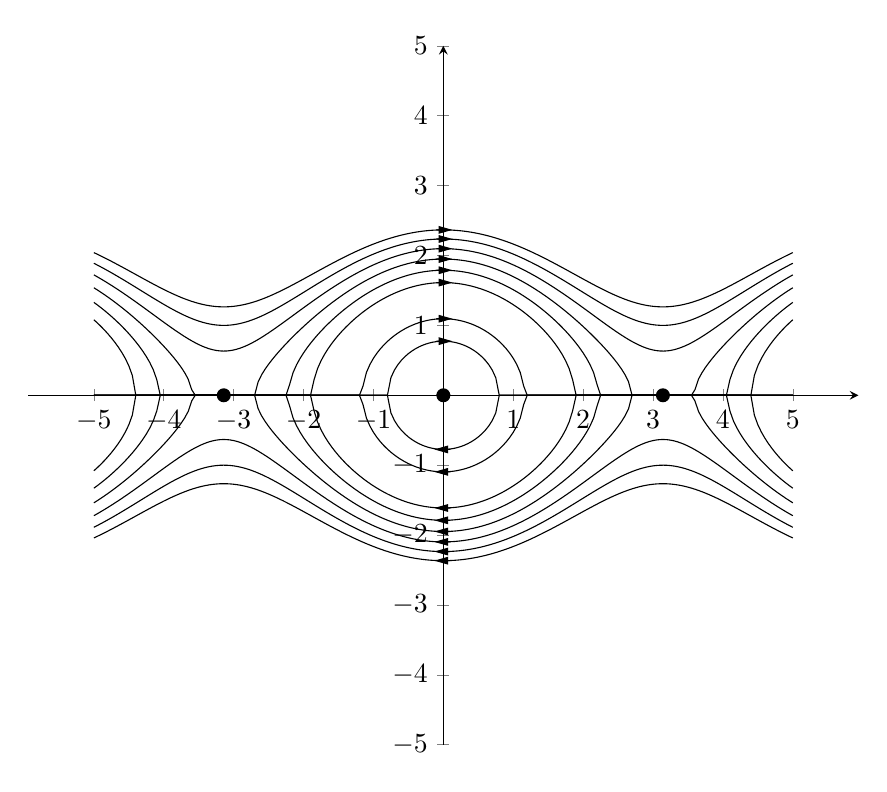
\begin{tikzpicture}


  \begin{axis}[%
    width=\textwidth,
    axis equal,
    axis lines=middle,
    xmin=-5,
    xmax=5,
    ymin=-5,
    ymax=5,
    axis background/.style={fill=white}
    ]
    \fill [black] (0,0) circle (0.1);
    \fill [black] (3.14156,0) circle (0.1);
    \fill [black] (-3.14156,0) circle (0.1);

  \addplot [color=black, forget plot]
    table[row sep=crcr]{%
  -5	0\\
  -4.95	0\\
  -4.9	0\\
  -4.85	0\\
  -4.8	0\\
  -4.75	0\\
  -4.7	0\\
  -4.65	0\\
  -4.6	0\\
  -4.55	0\\
  -4.5	0\\
  -4.45	0\\
  -4.4	0\\
  -4.35	0\\
  -4.3	0\\
  -4.25	0\\
  -4.2	0\\
  -4.15	0\\
  -4.1	0\\
  -4.05	0\\
  -4	0\\
  -3.95	0\\
  -3.9	0\\
  -3.85	0\\
  -3.8	0\\
  -3.75	0\\
  -3.7	0\\
  -3.65	0\\
  -3.6	0\\
  -3.55	0\\
  -3.5	0\\
  -3.45	0\\
  -3.4	0\\
  -3.35	0\\
  -3.3	0\\
  -3.25	0\\
  -3.2	0\\
  -3.15	0\\
  -3.1	0\\
  -3.05	0\\
  -3	0\\
  -2.95	0\\
  -2.9	0\\
  -2.85	0\\
  -2.8	0\\
  -2.75	0\\
  -2.7	0\\
  -2.65	0\\
  -2.6	0\\
  -2.55	0\\
  -2.5	0\\
  -2.45	0\\
  -2.4	0\\
  -2.35	0\\
  -2.3	0\\
  -2.25	0\\
  -2.2	0\\
  -2.15	0\\
  -2.1	0\\
  -2.05	0\\
  -2	0\\
  -1.95	0\\
  -1.9	0\\
  -1.85	0\\
  -1.8	0\\
  -1.75	0\\
  -1.7	0\\
  -1.65	0\\
  -1.6	0\\
  -1.55	0\\
  -1.5	0\\
  -1.45	0\\
  -1.4	0\\
  -1.35	0\\
  -1.3	0\\
  -1.25	0\\
  -1.2	0\\
  -1.15	0\\
  -1.1	0\\
  -1.05	0\\
  -1	0\\
  -0.95	0\\
  -0.899999999999999	0\\
  -0.85	0\\
  -0.8	0\\
  -0.75	0\\
  -0.7	0\\
  -0.649999999999999	0\\
  -0.6	0\\
  -0.55	0\\
  -0.5	0\\
  -0.45	0\\
  -0.399999999999999	0\\
  -0.35	0\\
  -0.3	0\\
  -0.25	0\\
  -0.199999999999999	0\\
  -0.149999999999999	0\\
  -0.0999999999999996	0\\
  -0.0499999999999998	0\\
  0	0\\
  0.0499999999999998	0\\
  0.0999999999999996	0\\
  0.149999999999999	0\\
  0.199999999999999	0\\
  0.25	0\\
  0.3	0\\
  0.35	0\\
  0.399999999999999	0\\
  0.45	0\\
  0.5	0\\
  0.55	0\\
  0.6	0\\
  0.649999999999999	0\\
  0.7	0\\
  0.75	0\\
  0.8	0\\
  0.85	0\\
  0.899999999999999	0\\
  0.95	0\\
  1	0\\
  1.05	0\\
  1.1	0\\
  1.15	0\\
  1.2	0\\
  1.25	0\\
  1.3	0\\
  1.35	0\\
  1.4	0\\
  1.45	0\\
  1.5	0\\
  1.55	0\\
  1.6	0\\
  1.65	0\\
  1.7	0\\
  1.75	0\\
  1.8	0\\
  1.85	0\\
  1.9	0\\
  1.95	0\\
  2	0\\
  2.05	0\\
  2.1	0\\
  2.15	0\\
  2.2	0\\
  2.25	0\\
  2.3	0\\
  2.35	0\\
  2.4	0\\
  2.45	0\\
  2.5	0\\
  2.55	0\\
  2.6	0\\
  2.65	0\\
  2.7	0\\
  2.75	0\\
  2.8	0\\
  2.85	0\\
  2.9	0\\
  2.95	0\\
  3	0\\
  3.05	0\\
  3.1	0\\
  3.15	0\\
  3.2	0\\
  3.25	0\\
  3.3	0\\
  3.35	0\\
  3.4	0\\
  3.45	0\\
  3.5	0\\
  3.55	0\\
  3.6	0\\
  3.65	0\\
  3.7	0\\
  3.75	0\\
  3.8	0\\
  3.85	0\\
  3.9	0\\
  3.95	0\\
  4	0\\
  4.05	0\\
  4.1	0\\
  4.15	0\\
  4.2	0\\
  4.25	0\\
  4.3	0\\
  4.35	0\\
  4.4	0\\
  4.45	0\\
  4.5	0\\
  4.55	0\\
  4.6	0\\
  4.65	0\\
  4.7	0\\
  4.75	0\\
  4.8	0\\
  4.85	0\\
  4.9	0\\
  4.95	0\\
  5	0\\
  };
  \addplot [color=black, forget plot]
    table[row sep=crcr]{%
  -5	-0\\
  -4.95	-0\\
  -4.9	-0\\
  -4.85	-0\\
  -4.8	-0\\
  -4.75	-0\\
  -4.7	-0\\
  -4.65	-0\\
  -4.6	-0\\
  -4.55	-0\\
  -4.5	-0\\
  -4.45	-0\\
  -4.4	-0\\
  -4.35	-0\\
  -4.3	-0\\
  -4.25	-0\\
  -4.2	-0\\
  -4.15	-0\\
  -4.1	-0\\
  -4.05	-0\\
  -4	-0\\
  -3.95	-0\\
  -3.9	-0\\
  -3.85	-0\\
  -3.8	-0\\
  -3.75	-0\\
  -3.7	-0\\
  -3.65	-0\\
  -3.6	-0\\
  -3.55	-0\\
  -3.5	-0\\
  -3.45	-0\\
  -3.4	-0\\
  -3.35	-0\\
  -3.3	-0\\
  -3.25	-0\\
  -3.2	-0\\
  -3.15	-0\\
  -3.1	-0\\
  -3.05	-0\\
  -3	-0\\
  -2.95	-0\\
  -2.9	-0\\
  -2.85	-0\\
  -2.8	-0\\
  -2.75	-0\\
  -2.7	-0\\
  -2.65	-0\\
  -2.6	-0\\
  -2.55	-0\\
  -2.5	-0\\
  -2.45	-0\\
  -2.4	-0\\
  -2.35	-0\\
  -2.3	-0\\
  -2.25	-0\\
  -2.2	-0\\
  -2.15	-0\\
  -2.1	-0\\
  -2.05	-0\\
  -2	-0\\
  -1.95	-0\\
  -1.9	-0\\
  -1.85	-0\\
  -1.8	-0\\
  -1.75	-0\\
  -1.7	-0\\
  -1.65	-0\\
  -1.6	-0\\
  -1.55	-0\\
  -1.5	-0\\
  -1.45	-0\\
  -1.4	-0\\
  -1.35	-0\\
  -1.3	-0\\
  -1.25	-0\\
  -1.2	-0\\
  -1.15	-0\\
  -1.1	-0\\
  -1.05	-0\\
  -1	-0\\
  -0.95	-0\\
  -0.899999999999999	-0\\
  -0.85	-0\\
  -0.8	-0\\
  -0.75	-0\\
  -0.7	-0\\
  -0.649999999999999	-0\\
  -0.6	-0\\
  -0.55	-0\\
  -0.5	-0\\
  -0.45	-0\\
  -0.399999999999999	-0\\
  -0.35	-0\\
  -0.3	-0\\
  -0.25	-0\\
  -0.199999999999999	-0\\
  -0.149999999999999	-0\\
  -0.0999999999999996	-0\\
  -0.0499999999999998	-0\\
  0	-0\\
  0.0499999999999998	-0\\
  0.0999999999999996	-0\\
  0.149999999999999	-0\\
  0.199999999999999	-0\\
  0.25	-0\\
  0.3	-0\\
  0.35	-0\\
  0.399999999999999	-0\\
  0.45	-0\\
  0.5	-0\\
  0.55	-0\\
  0.6	-0\\
  0.649999999999999	-0\\
  0.7	-0\\
  0.75	-0\\
  0.8	-0\\
  0.85	-0\\
  0.899999999999999	-0\\
  0.95	-0\\
  1	-0\\
  1.05	-0\\
  1.1	-0\\
  1.15	-0\\
  1.2	-0\\
  1.25	-0\\
  1.3	-0\\
  1.35	-0\\
  1.4	-0\\
  1.45	-0\\
  1.5	-0\\
  1.55	-0\\
  1.6	-0\\
  1.65	-0\\
  1.7	-0\\
  1.75	-0\\
  1.8	-0\\
  1.85	-0\\
  1.9	-0\\
  1.95	-0\\
  2	-0\\
  2.05	-0\\
  2.1	-0\\
  2.15	-0\\
  2.2	-0\\
  2.25	-0\\
  2.3	-0\\
  2.35	-0\\
  2.4	-0\\
  2.45	-0\\
  2.5	-0\\
  2.55	-0\\
  2.6	-0\\
  2.65	-0\\
  2.7	-0\\
  2.75	-0\\
  2.8	-0\\
  2.85	-0\\
  2.9	-0\\
  2.95	-0\\
  3	-0\\
  3.05	-0\\
  3.1	-0\\
  3.15	-0\\
  3.2	-0\\
  3.25	-0\\
  3.3	-0\\
  3.35	-0\\
  3.4	-0\\
  3.45	-0\\
  3.5	-0\\
  3.55	-0\\
  3.6	-0\\
  3.65	-0\\
  3.7	-0\\
  3.75	-0\\
  3.8	-0\\
  3.85	-0\\
  3.9	-0\\
  3.95	-0\\
  4	-0\\
  4.05	-0\\
  4.1	-0\\
  4.15	-0\\
  4.2	-0\\
  4.25	-0\\
  4.3	-0\\
  4.35	-0\\
  4.4	-0\\
  4.45	-0\\
  4.5	-0\\
  4.55	-0\\
  4.6	-0\\
  4.65	-0\\
  4.7	-0\\
  4.75	-0\\
  4.8	-0\\
  4.85	-0\\
  4.9	-0\\
  4.95	-0\\
  5	-0\\
  };
  
  \addplot[area legend, draw=black, fill=black, forget plot]
  table[row sep=crcr] {%
  x	y\\
  -0.0806451612903221	-1.11022302462516e-16\\
  -0.0999999999999996	-1.11022302462516e-16\\
  -0.0999999999999996	-1.11022302462516e-16\\
  -0.0999999999999996	-1.11022302462516e-16\\
  -0.0999999999999996	-1.11022302462516e-16\\
  -0.0999999999999996	-1.11022302462516e-16\\
  -0.0612903225806445	-1.11022302462516e-16\\
  -0.0612903225806445	-0.0117278276383972\\
  0.0999999999999996	-1.11022302462516e-16\\
  -0.0612903225806436	0.0117278276383972\\
  -0.0612903225806445	-1.11022302462516e-16\\
  }--cycle;
  
  \addplot[area legend, draw=black, fill=black, forget plot]
  table[row sep=crcr] {%
  x	y\\
  0.080645161290323	-1.73472347597681e-18\\
  0.0999999999999996	-1.73472347597681e-18\\
  0.0999999999999996	-1.73472347597681e-18\\
  0.0999999999999996	-1.73472347597681e-18\\
  0.0999999999999996	-1.73472347597681e-18\\
  0.0999999999999996	-1.73472347597681e-18\\
  0.0612903225806463	-1.73472347597681e-18\\
  0.0612903225806463	-0.000175917414575958\\
  -0.0999999999999996	-1.73472347597681e-18\\
  0.0612903225806463	0.000175917414575958\\
  0.0612903225806463	-1.73472347597681e-18\\
  }--cycle;
  \addplot [color=black, forget plot]
    table[row sep=crcr]{%
  -5	0\\
  -4.95	0\\
  -4.9	0\\
  -4.85	0\\
  -4.8	0\\
  -4.75	0\\
  -4.7	0\\
  -4.65	0\\
  -4.6	0\\
  -4.55	0\\
  -4.5	0\\
  -4.45	0\\
  -4.4	0\\
  -4.35	0\\
  -4.3	0\\
  -4.25	0\\
  -4.2	0\\
  -4.15	0\\
  -4.1	0\\
  -4.05	0\\
  -4	0\\
  -3.95	0\\
  -3.9	0\\
  -3.85	0\\
  -3.8	0\\
  -3.75	0\\
  -3.7	0\\
  -3.65	0\\
  -3.6	0\\
  -3.55	0\\
  -3.5	0\\
  -3.45	0\\
  -3.4	0\\
  -3.35	0\\
  -3.3	0\\
  -3.25	0\\
  -3.2	0\\
  -3.15	0\\
  -3.1	0\\
  -3.05	0\\
  -3	0\\
  -2.95	0\\
  -2.9	0\\
  -2.85	0\\
  -2.8	0\\
  -2.75	0\\
  -2.7	0\\
  -2.65	0\\
  -2.6	0\\
  -2.55	0\\
  -2.5	0\\
  -2.45	0\\
  -2.4	0\\
  -2.35	0\\
  -2.3	0\\
  -2.25	0\\
  -2.2	0\\
  -2.15	0\\
  -2.1	0\\
  -2.05	0\\
  -2	0\\
  -1.95	0\\
  -1.9	0\\
  -1.85	0\\
  -1.8	0\\
  -1.75	0\\
  -1.7	0\\
  -1.65	0\\
  -1.6	0\\
  -1.55	0\\
  -1.5	0\\
  -1.45	0\\
  -1.4	0\\
  -1.35	0\\
  -1.3	0\\
  -1.25	0\\
  -1.2	0\\
  -1.15	0\\
  -1.1	0\\
  -1.05	0\\
  -1	0\\
  -0.95	0\\
  -0.899999999999999	0\\
  -0.85	0\\
  -0.8	0\\
  -0.75	0.251749355009386\\
  -0.7	0.360117167834271\\
  -0.649999999999999	0.438369247436579\\
  -0.6	0.500670779873718\\
  -0.55	0.552312451533561\\
  -0.5	0.595957317079626\\
  -0.45	0.633162068277431\\
  -0.399999999999999	0.664922542861776\\
  -0.35	0.691914319619675\\
  -0.3	0.714613866539974\\
  -0.25	0.733365422842726\\
  -0.199999999999999	0.748420440449406\\
  -0.149999999999999	0.75996194369987\\
  -0.0999999999999996	0.76811999749782\\
  -0.0499999999999998	0.772981578557945\\
  0	0.774596669241483\\
  0.0499999999999998	0.772981578557945\\
  0.0999999999999996	0.76811999749782\\
  0.149999999999999	0.75996194369987\\
  0.199999999999999	0.748420440449406\\
  0.25	0.733365422842726\\
  0.3	0.714613866539974\\
  0.35	0.691914319619675\\
  0.399999999999999	0.664922542861776\\
  0.45	0.633162068277431\\
  0.5	0.595957317079626\\
  0.55	0.552312451533561\\
  0.6	0.500670779873718\\
  0.649999999999999	0.438369247436579\\
  0.7	0.360117167834271\\
  0.75	0.251749355009386\\
  0.8	0\\
  0.85	0\\
  0.899999999999999	0\\
  0.95	0\\
  1	0\\
  1.05	0\\
  1.1	0\\
  1.15	0\\
  1.2	0\\
  1.25	0\\
  1.3	0\\
  1.35	0\\
  1.4	0\\
  1.45	0\\
  1.5	0\\
  1.55	0\\
  1.6	0\\
  1.65	0\\
  1.7	0\\
  1.75	0\\
  1.8	0\\
  1.85	0\\
  1.9	0\\
  1.95	0\\
  2	0\\
  2.05	0\\
  2.1	0\\
  2.15	0\\
  2.2	0\\
  2.25	0\\
  2.3	0\\
  2.35	0\\
  2.4	0\\
  2.45	0\\
  2.5	0\\
  2.55	0\\
  2.6	0\\
  2.65	0\\
  2.7	0\\
  2.75	0\\
  2.8	0\\
  2.85	0\\
  2.9	0\\
  2.95	0\\
  3	0\\
  3.05	0\\
  3.1	0\\
  3.15	0\\
  3.2	0\\
  3.25	0\\
  3.3	0\\
  3.35	0\\
  3.4	0\\
  3.45	0\\
  3.5	0\\
  3.55	0\\
  3.6	0\\
  3.65	0\\
  3.7	0\\
  3.75	0\\
  3.8	0\\
  3.85	0\\
  3.9	0\\
  3.95	0\\
  4	0\\
  4.05	0\\
  4.1	0\\
  4.15	0\\
  4.2	0\\
  4.25	0\\
  4.3	0\\
  4.35	0\\
  4.4	0\\
  4.45	0\\
  4.5	0\\
  4.55	0\\
  4.6	0\\
  4.65	0\\
  4.7	0\\
  4.75	0\\
  4.8	0\\
  4.85	0\\
  4.9	0\\
  4.95	0\\
  5	0\\
  };
  \addplot [color=black, forget plot]
    table[row sep=crcr]{%
  -5	-0\\
  -4.95	-0\\
  -4.9	-0\\
  -4.85	-0\\
  -4.8	-0\\
  -4.75	-0\\
  -4.7	-0\\
  -4.65	-0\\
  -4.6	-0\\
  -4.55	-0\\
  -4.5	-0\\
  -4.45	-0\\
  -4.4	-0\\
  -4.35	-0\\
  -4.3	-0\\
  -4.25	-0\\
  -4.2	-0\\
  -4.15	-0\\
  -4.1	-0\\
  -4.05	-0\\
  -4	-0\\
  -3.95	-0\\
  -3.9	-0\\
  -3.85	-0\\
  -3.8	-0\\
  -3.75	-0\\
  -3.7	-0\\
  -3.65	-0\\
  -3.6	-0\\
  -3.55	-0\\
  -3.5	-0\\
  -3.45	-0\\
  -3.4	-0\\
  -3.35	-0\\
  -3.3	-0\\
  -3.25	-0\\
  -3.2	-0\\
  -3.15	-0\\
  -3.1	-0\\
  -3.05	-0\\
  -3	-0\\
  -2.95	-0\\
  -2.9	-0\\
  -2.85	-0\\
  -2.8	-0\\
  -2.75	-0\\
  -2.7	-0\\
  -2.65	-0\\
  -2.6	-0\\
  -2.55	-0\\
  -2.5	-0\\
  -2.45	-0\\
  -2.4	-0\\
  -2.35	-0\\
  -2.3	-0\\
  -2.25	-0\\
  -2.2	-0\\
  -2.15	-0\\
  -2.1	-0\\
  -2.05	-0\\
  -2	-0\\
  -1.95	-0\\
  -1.9	-0\\
  -1.85	-0\\
  -1.8	-0\\
  -1.75	-0\\
  -1.7	-0\\
  -1.65	-0\\
  -1.6	-0\\
  -1.55	-0\\
  -1.5	-0\\
  -1.45	-0\\
  -1.4	-0\\
  -1.35	-0\\
  -1.3	-0\\
  -1.25	-0\\
  -1.2	-0\\
  -1.15	-0\\
  -1.1	-0\\
  -1.05	-0\\
  -1	-0\\
  -0.95	-0\\
  -0.899999999999999	-0\\
  -0.85	-0\\
  -0.8	-0\\
  -0.75	-0.251749355009386\\
  -0.7	-0.360117167834271\\
  -0.649999999999999	-0.438369247436579\\
  -0.6	-0.500670779873718\\
  -0.55	-0.552312451533561\\
  -0.5	-0.595957317079626\\
  -0.45	-0.633162068277431\\
  -0.399999999999999	-0.664922542861776\\
  -0.35	-0.691914319619675\\
  -0.3	-0.714613866539974\\
  -0.25	-0.733365422842726\\
  -0.199999999999999	-0.748420440449406\\
  -0.149999999999999	-0.75996194369987\\
  -0.0999999999999996	-0.76811999749782\\
  -0.0499999999999998	-0.772981578557945\\
  0	-0.774596669241483\\
  0.0499999999999998	-0.772981578557945\\
  0.0999999999999996	-0.76811999749782\\
  0.149999999999999	-0.75996194369987\\
  0.199999999999999	-0.748420440449406\\
  0.25	-0.733365422842726\\
  0.3	-0.714613866539974\\
  0.35	-0.691914319619675\\
  0.399999999999999	-0.664922542861776\\
  0.45	-0.633162068277431\\
  0.5	-0.595957317079626\\
  0.55	-0.552312451533561\\
  0.6	-0.500670779873718\\
  0.649999999999999	-0.438369247436579\\
  0.7	-0.360117167834271\\
  0.75	-0.251749355009386\\
  0.8	-0\\
  0.85	-0\\
  0.899999999999999	-0\\
  0.95	-0\\
  1	-0\\
  1.05	-0\\
  1.1	-0\\
  1.15	-0\\
  1.2	-0\\
  1.25	-0\\
  1.3	-0\\
  1.35	-0\\
  1.4	-0\\
  1.45	-0\\
  1.5	-0\\
  1.55	-0\\
  1.6	-0\\
  1.65	-0\\
  1.7	-0\\
  1.75	-0\\
  1.8	-0\\
  1.85	-0\\
  1.9	-0\\
  1.95	-0\\
  2	-0\\
  2.05	-0\\
  2.1	-0\\
  2.15	-0\\
  2.2	-0\\
  2.25	-0\\
  2.3	-0\\
  2.35	-0\\
  2.4	-0\\
  2.45	-0\\
  2.5	-0\\
  2.55	-0\\
  2.6	-0\\
  2.65	-0\\
  2.7	-0\\
  2.75	-0\\
  2.8	-0\\
  2.85	-0\\
  2.9	-0\\
  2.95	-0\\
  3	-0\\
  3.05	-0\\
  3.1	-0\\
  3.15	-0\\
  3.2	-0\\
  3.25	-0\\
  3.3	-0\\
  3.35	-0\\
  3.4	-0\\
  3.45	-0\\
  3.5	-0\\
  3.55	-0\\
  3.6	-0\\
  3.65	-0\\
  3.7	-0\\
  3.75	-0\\
  3.8	-0\\
  3.85	-0\\
  3.9	-0\\
  3.95	-0\\
  4	-0\\
  4.05	-0\\
  4.1	-0\\
  4.15	-0\\
  4.2	-0\\
  4.25	-0\\
  4.3	-0\\
  4.35	-0\\
  4.4	-0\\
  4.45	-0\\
  4.5	-0\\
  4.55	-0\\
  4.6	-0\\
  4.65	-0\\
  4.7	-0\\
  4.75	-0\\
  4.8	-0\\
  4.85	-0\\
  4.9	-0\\
  4.95	-0\\
  5	-0\\
  };
  
  \addplot[area legend, draw=black, fill=black, forget plot]
  table[row sep=crcr] {%
  x	y\\
  -0.0806451612903221	0.774596669241484\\
  -0.0999999999999996	0.774596669241484\\
  -0.0999999999999996	0.774596669241484\\
  -0.0999999999999996	0.774596669241484\\
  -0.0999999999999996	0.774596669241484\\
  -0.0999999999999996	0.774596669241484\\
  -0.0612903225806445	0.774596669241484\\
  -0.0612903225806445	0.728347413473933\\
  0.0999999999999996	0.774596669241484\\
  -0.0612903225806436	0.820845925009034\\
  -0.0612903225806445	0.774596669241484\\
  }--cycle;
  
  \addplot[area legend, draw=black, fill=black, forget plot]
  table[row sep=crcr] {%
  x	y\\
  0.080645161290323	-0.774596669241483\\
  0.0999999999999996	-0.774596669241483\\
  0.0999999999999996	-0.774596669241483\\
  0.0999999999999996	-0.774596669241483\\
  0.0999999999999996	-0.774596669241483\\
  0.0999999999999996	-0.774596669241483\\
  0.0612903225806463	-0.774596669241483\\
  0.0612903225806463	-0.820845925009033\\
  -0.0999999999999996	-0.774596669241483\\
  0.0612903225806463	-0.728347413473934\\
  0.0612903225806463	-0.774596669241483\\
  }--cycle;
  \addplot [color=black, forget plot]
    table[row sep=crcr]{%
  -5	0\\
  -4.95	0\\
  -4.9	0\\
  -4.85	0\\
  -4.8	0\\
  -4.75	0\\
  -4.7	0\\
  -4.65	0\\
  -4.6	0\\
  -4.55	0\\
  -4.5	0\\
  -4.45	0\\
  -4.4	0\\
  -4.35	0\\
  -4.3	0\\
  -4.25	0\\
  -4.2	0\\
  -4.15	0\\
  -4.1	0\\
  -4.05	0\\
  -4	0\\
  -3.95	0\\
  -3.9	0\\
  -3.85	0\\
  -3.8	0\\
  -3.75	0\\
  -3.7	0\\
  -3.65	0\\
  -3.6	0\\
  -3.55	0\\
  -3.5	0\\
  -3.45	0\\
  -3.4	0\\
  -3.35	0\\
  -3.3	0\\
  -3.25	0\\
  -3.2	0\\
  -3.15	0\\
  -3.1	0\\
  -3.05	0\\
  -3	0\\
  -2.95	0\\
  -2.9	0\\
  -2.85	0\\
  -2.8	0\\
  -2.75	0\\
  -2.7	0\\
  -2.65	0\\
  -2.6	0\\
  -2.55	0\\
  -2.5	0\\
  -2.45	0\\
  -2.4	0\\
  -2.35	0\\
  -2.3	0\\
  -2.25	0\\
  -2.2	0\\
  -2.15	0\\
  -2.1	0\\
  -2.05	0\\
  -2	0\\
  -1.95	0\\
  -1.9	0\\
  -1.85	0\\
  -1.8	0\\
  -1.75	0\\
  -1.7	0\\
  -1.65	0\\
  -1.6	0\\
  -1.55	0\\
  -1.5	0\\
  -1.45	0\\
  -1.4	0\\
  -1.35	0\\
  -1.3	0\\
  -1.25	0\\
  -1.2	0\\
  -1.15	0.130287688475599\\
  -1.1	0.327402264578539\\
  -1.05	0.441748905809006\\
  -1	0.529721258527803\\
  -0.95	0.602798622201284\\
  -0.899999999999999	0.665747652298774\\
  -0.85	0.721086882261746\\
  -0.8	0.770333316619716\\
  -0.75	0.81448004134395\\
  -0.7	0.854215648749762\\
  -0.649999999999999	0.890037975087643\\
  -0.6	0.922318399371582\\
  -0.55	0.95134065618947\\
  -0.5	0.977325495308879\\
  -0.45	1.00044700244708\\
  -0.399999999999999	1.02084376277948\\
  -0.35	1.03862670180135\\
  -0.3	1.05388470823483\\
  -0.25	1.06668872845891\\
  -0.199999999999999	1.07709477562677\\
  -0.149999999999999	1.08514614493721\\
  -0.0999999999999996	1.090875029761\\
  -0.0499999999999998	1.09430366936693\\
  0	1.09544511501033\\
  0.0499999999999998	1.09430366936693\\
  0.0999999999999996	1.090875029761\\
  0.149999999999999	1.08514614493721\\
  0.199999999999999	1.07709477562677\\
  0.25	1.06668872845891\\
  0.3	1.05388470823483\\
  0.35	1.03862670180135\\
  0.399999999999999	1.02084376277948\\
  0.45	1.00044700244708\\
  0.5	0.977325495308879\\
  0.55	0.95134065618947\\
  0.6	0.922318399371582\\
  0.649999999999999	0.890037975087643\\
  0.7	0.854215648749762\\
  0.75	0.81448004134395\\
  0.8	0.770333316619716\\
  0.85	0.721086882261746\\
  0.899999999999999	0.665747652298774\\
  0.95	0.602798622201284\\
  1	0.529721258527803\\
  1.05	0.441748905809006\\
  1.1	0.327402264578539\\
  1.15	0.130287688475599\\
  1.2	0\\
  1.25	0\\
  1.3	0\\
  1.35	0\\
  1.4	0\\
  1.45	0\\
  1.5	0\\
  1.55	0\\
  1.6	0\\
  1.65	0\\
  1.7	0\\
  1.75	0\\
  1.8	0\\
  1.85	0\\
  1.9	0\\
  1.95	0\\
  2	0\\
  2.05	0\\
  2.1	0\\
  2.15	0\\
  2.2	0\\
  2.25	0\\
  2.3	0\\
  2.35	0\\
  2.4	0\\
  2.45	0\\
  2.5	0\\
  2.55	0\\
  2.6	0\\
  2.65	0\\
  2.7	0\\
  2.75	0\\
  2.8	0\\
  2.85	0\\
  2.9	0\\
  2.95	0\\
  3	0\\
  3.05	0\\
  3.1	0\\
  3.15	0\\
  3.2	0\\
  3.25	0\\
  3.3	0\\
  3.35	0\\
  3.4	0\\
  3.45	0\\
  3.5	0\\
  3.55	0\\
  3.6	0\\
  3.65	0\\
  3.7	0\\
  3.75	0\\
  3.8	0\\
  3.85	0\\
  3.9	0\\
  3.95	0\\
  4	0\\
  4.05	0\\
  4.1	0\\
  4.15	0\\
  4.2	0\\
  4.25	0\\
  4.3	0\\
  4.35	0\\
  4.4	0\\
  4.45	0\\
  4.5	0\\
  4.55	0\\
  4.6	0\\
  4.65	0\\
  4.7	0\\
  4.75	0\\
  4.8	0\\
  4.85	0\\
  4.9	0\\
  4.95	0\\
  5	0\\
  };
  \addplot [color=black, forget plot]
    table[row sep=crcr]{%
  -5	-0\\
  -4.95	-0\\
  -4.9	-0\\
  -4.85	-0\\
  -4.8	-0\\
  -4.75	-0\\
  -4.7	-0\\
  -4.65	-0\\
  -4.6	-0\\
  -4.55	-0\\
  -4.5	-0\\
  -4.45	-0\\
  -4.4	-0\\
  -4.35	-0\\
  -4.3	-0\\
  -4.25	-0\\
  -4.2	-0\\
  -4.15	-0\\
  -4.1	-0\\
  -4.05	-0\\
  -4	-0\\
  -3.95	-0\\
  -3.9	-0\\
  -3.85	-0\\
  -3.8	-0\\
  -3.75	-0\\
  -3.7	-0\\
  -3.65	-0\\
  -3.6	-0\\
  -3.55	-0\\
  -3.5	-0\\
  -3.45	-0\\
  -3.4	-0\\
  -3.35	-0\\
  -3.3	-0\\
  -3.25	-0\\
  -3.2	-0\\
  -3.15	-0\\
  -3.1	-0\\
  -3.05	-0\\
  -3	-0\\
  -2.95	-0\\
  -2.9	-0\\
  -2.85	-0\\
  -2.8	-0\\
  -2.75	-0\\
  -2.7	-0\\
  -2.65	-0\\
  -2.6	-0\\
  -2.55	-0\\
  -2.5	-0\\
  -2.45	-0\\
  -2.4	-0\\
  -2.35	-0\\
  -2.3	-0\\
  -2.25	-0\\
  -2.2	-0\\
  -2.15	-0\\
  -2.1	-0\\
  -2.05	-0\\
  -2	-0\\
  -1.95	-0\\
  -1.9	-0\\
  -1.85	-0\\
  -1.8	-0\\
  -1.75	-0\\
  -1.7	-0\\
  -1.65	-0\\
  -1.6	-0\\
  -1.55	-0\\
  -1.5	-0\\
  -1.45	-0\\
  -1.4	-0\\
  -1.35	-0\\
  -1.3	-0\\
  -1.25	-0\\
  -1.2	-0\\
  -1.15	-0.130287688475599\\
  -1.1	-0.327402264578539\\
  -1.05	-0.441748905809006\\
  -1	-0.529721258527803\\
  -0.95	-0.602798622201284\\
  -0.899999999999999	-0.665747652298774\\
  -0.85	-0.721086882261746\\
  -0.8	-0.770333316619716\\
  -0.75	-0.81448004134395\\
  -0.7	-0.854215648749762\\
  -0.649999999999999	-0.890037975087643\\
  -0.6	-0.922318399371582\\
  -0.55	-0.95134065618947\\
  -0.5	-0.977325495308879\\
  -0.45	-1.00044700244708\\
  -0.399999999999999	-1.02084376277948\\
  -0.35	-1.03862670180135\\
  -0.3	-1.05388470823483\\
  -0.25	-1.06668872845891\\
  -0.199999999999999	-1.07709477562677\\
  -0.149999999999999	-1.08514614493721\\
  -0.0999999999999996	-1.090875029761\\
  -0.0499999999999998	-1.09430366936693\\
  0	-1.09544511501033\\
  0.0499999999999998	-1.09430366936693\\
  0.0999999999999996	-1.090875029761\\
  0.149999999999999	-1.08514614493721\\
  0.199999999999999	-1.07709477562677\\
  0.25	-1.06668872845891\\
  0.3	-1.05388470823483\\
  0.35	-1.03862670180135\\
  0.399999999999999	-1.02084376277948\\
  0.45	-1.00044700244708\\
  0.5	-0.977325495308879\\
  0.55	-0.95134065618947\\
  0.6	-0.922318399371582\\
  0.649999999999999	-0.890037975087643\\
  0.7	-0.854215648749762\\
  0.75	-0.81448004134395\\
  0.8	-0.770333316619716\\
  0.85	-0.721086882261746\\
  0.899999999999999	-0.665747652298774\\
  0.95	-0.602798622201284\\
  1	-0.529721258527803\\
  1.05	-0.441748905809006\\
  1.1	-0.327402264578539\\
  1.15	-0.130287688475599\\
  1.2	-0\\
  1.25	-0\\
  1.3	-0\\
  1.35	-0\\
  1.4	-0\\
  1.45	-0\\
  1.5	-0\\
  1.55	-0\\
  1.6	-0\\
  1.65	-0\\
  1.7	-0\\
  1.75	-0\\
  1.8	-0\\
  1.85	-0\\
  1.9	-0\\
  1.95	-0\\
  2	-0\\
  2.05	-0\\
  2.1	-0\\
  2.15	-0\\
  2.2	-0\\
  2.25	-0\\
  2.3	-0\\
  2.35	-0\\
  2.4	-0\\
  2.45	-0\\
  2.5	-0\\
  2.55	-0\\
  2.6	-0\\
  2.65	-0\\
  2.7	-0\\
  2.75	-0\\
  2.8	-0\\
  2.85	-0\\
  2.9	-0\\
  2.95	-0\\
  3	-0\\
  3.05	-0\\
  3.1	-0\\
  3.15	-0\\
  3.2	-0\\
  3.25	-0\\
  3.3	-0\\
  3.35	-0\\
  3.4	-0\\
  3.45	-0\\
  3.5	-0\\
  3.55	-0\\
  3.6	-0\\
  3.65	-0\\
  3.7	-0\\
  3.75	-0\\
  3.8	-0\\
  3.85	-0\\
  3.9	-0\\
  3.95	-0\\
  4	-0\\
  4.05	-0\\
  4.1	-0\\
  4.15	-0\\
  4.2	-0\\
  4.25	-0\\
  4.3	-0\\
  4.35	-0\\
  4.4	-0\\
  4.45	-0\\
  4.5	-0\\
  4.55	-0\\
  4.6	-0\\
  4.65	-0\\
  4.7	-0\\
  4.75	-0\\
  4.8	-0\\
  4.85	-0\\
  4.9	-0\\
  4.95	-0\\
  5	-0\\
  };
  
  \addplot[area legend, draw=black, fill=black, forget plot]
  table[row sep=crcr] {%
  x	y\\
  -0.0806451612903221	1.09544511501033\\
  -0.0999999999999996	1.09544511501033\\
  -0.0999999999999996	1.09544511501033\\
  -0.0999999999999996	1.09544511501033\\
  -0.0999999999999996	1.09544511501033\\
  -0.0999999999999996	1.09544511501033\\
  -0.0612903225806445	1.09544511501033\\
  -0.0612903225806445	1.04919585924278\\
  0.0999999999999996	1.09544511501033\\
  -0.0612903225806436	1.14169437077788\\
  -0.0612903225806445	1.09544511501033\\
  }--cycle;
  
  \addplot[area legend, draw=black, fill=black, forget plot]
  table[row sep=crcr] {%
  x	y\\
  0.080645161290323	-1.09544511501033\\
  0.0999999999999996	-1.09544511501033\\
  0.0999999999999996	-1.09544511501033\\
  0.0999999999999996	-1.09544511501033\\
  0.0999999999999996	-1.09544511501033\\
  0.0999999999999996	-1.09544511501033\\
  0.0612903225806463	-1.09544511501033\\
  0.0612903225806463	-1.14169437077788\\
  -0.0999999999999996	-1.09544511501033\\
  0.0612903225806463	-1.04919585924278\\
  0.0612903225806463	-1.09544511501033\\
  }--cycle;
  \addplot [color=black, forget plot]
    table[row sep=crcr]{%
  -5	1.08042786474917\\
  -4.95	1.03477673239637\\
  -4.9	0.986420163442106\\
  -4.85	0.935069101297767\\
  -4.8	0.880339688347\\
  -4.75	0.821708163386462\\
  -4.7	0.758434356470103\\
  -4.65	0.689422200676782\\
  -4.6	0.612939594193335\\
  -4.55	0.52597297201722\\
  -4.5	0.422384186657645\\
  -4.45	0.284996481418188\\
  -4.4	0\\
  -4.35	0\\
  -4.3	0\\
  -4.25	0\\
  -4.2	0\\
  -4.15	0\\
  -4.1	0\\
  -4.05	0\\
  -4	0\\
  -3.95	0\\
  -3.9	0\\
  -3.85	0\\
  -3.8	0\\
  -3.75	0\\
  -3.7	0\\
  -3.65	0\\
  -3.6	0\\
  -3.55	0\\
  -3.5	0\\
  -3.45	0\\
  -3.4	0\\
  -3.35	0\\
  -3.3	0\\
  -3.25	0\\
  -3.2	0\\
  -3.15	0\\
  -3.1	0\\
  -3.05	0\\
  -3	0\\
  -2.95	0\\
  -2.9	0\\
  -2.85	0\\
  -2.8	0\\
  -2.75	0\\
  -2.7	0\\
  -2.65	0\\
  -2.6	0\\
  -2.55	0\\
  -2.5	0\\
  -2.45	0\\
  -2.4	0\\
  -2.35	0\\
  -2.3	0\\
  -2.25	0\\
  -2.2	0\\
  -2.15	0\\
  -2.1	0\\
  -2.05	0\\
  -2	0\\
  -1.95	0\\
  -1.9	0\\
  -1.85	0.220951366483611\\
  -1.8	0.381570190939788\\
  -1.75	0.493465184892527\\
  -1.7	0.585073509406255\\
  -1.65	0.664648946727919\\
  -1.6	0.73593542882336\\
  -1.55	0.800992918574306\\
  -1.5	0.861089079791055\\
  -1.45	0.917063541274395\\
  -1.4	0.96950208138017\\
  -1.35	1.01882941368322\\
  -1.3	1.06536268812512\\
  -1.25	1.10934427694496\\
  -1.2	1.15096286167424\\
  -1.15	1.19036754062278\\
  -1.1	1.22767758098417\\
  -1.05	1.26298934903801\\
  -1	1.29638135274165\\
  -0.95	1.32791798652167\\
  -0.899999999999999	1.35765236218309\\
  -0.85	1.38562848259191\\
  -0.8	1.41188293377827\\
  -0.75	1.43644621818836\\
  -0.7	1.45934381643565\\
  -0.649999999999999	1.48059704075691\\
  -0.6	1.50022372658859\\
  -0.55	1.51823879680339\\
  -0.5	1.53465472461422\\
  -0.45	1.5494819149333\\
  -0.399999999999999	1.56272901937789\\
  -0.35	1.57440319667319\\
  -0.3	1.58451032759374\\
  -0.25	1.59305519158041\\
  -0.199999999999999	1.6000416106097\\
  -0.149999999999999	1.60547256465879\\
  -0.0999999999999996	1.60935028211886\\
  -0.0499999999999998	1.61167630769641\\
  0	1.61245154965971\\
  0.0499999999999998	1.61167630769641\\
  0.0999999999999996	1.60935028211886\\
  0.149999999999999	1.60547256465879\\
  0.199999999999999	1.6000416106097\\
  0.25	1.59305519158041\\
  0.3	1.58451032759374\\
  0.35	1.57440319667319\\
  0.399999999999999	1.56272901937789\\
  0.45	1.5494819149333\\
  0.5	1.53465472461422\\
  0.55	1.51823879680339\\
  0.6	1.50022372658859\\
  0.649999999999999	1.48059704075691\\
  0.7	1.45934381643565\\
  0.75	1.43644621818836\\
  0.8	1.41188293377827\\
  0.85	1.38562848259191\\
  0.899999999999999	1.35765236218309\\
  0.95	1.32791798652167\\
  1	1.29638135274165\\
  1.05	1.26298934903801\\
  1.1	1.22767758098417\\
  1.15	1.19036754062278\\
  1.2	1.15096286167424\\
  1.25	1.10934427694496\\
  1.3	1.06536268812512\\
  1.35	1.01882941368322\\
  1.4	0.96950208138017\\
  1.45	0.917063541274395\\
  1.5	0.861089079791055\\
  1.55	0.800992918574306\\
  1.6	0.73593542882336\\
  1.65	0.664648946727919\\
  1.7	0.585073509406255\\
  1.75	0.493465184892527\\
  1.8	0.381570190939788\\
  1.85	0.220951366483611\\
  1.9	0\\
  1.95	0\\
  2	0\\
  2.05	0\\
  2.1	0\\
  2.15	0\\
  2.2	0\\
  2.25	0\\
  2.3	0\\
  2.35	0\\
  2.4	0\\
  2.45	0\\
  2.5	0\\
  2.55	0\\
  2.6	0\\
  2.65	0\\
  2.7	0\\
  2.75	0\\
  2.8	0\\
  2.85	0\\
  2.9	0\\
  2.95	0\\
  3	0\\
  3.05	0\\
  3.1	0\\
  3.15	0\\
  3.2	0\\
  3.25	0\\
  3.3	0\\
  3.35	0\\
  3.4	0\\
  3.45	0\\
  3.5	0\\
  3.55	0\\
  3.6	0\\
  3.65	0\\
  3.7	0\\
  3.75	0\\
  3.8	0\\
  3.85	0\\
  3.9	0\\
  3.95	0\\
  4	0\\
  4.05	0\\
  4.1	0\\
  4.15	0\\
  4.2	0\\
  4.25	0\\
  4.3	0\\
  4.35	0\\
  4.4	0\\
  4.45	0.284996481418188\\
  4.5	0.422384186657645\\
  4.55	0.52597297201722\\
  4.6	0.612939594193335\\
  4.65	0.689422200676782\\
  4.7	0.758434356470103\\
  4.75	0.821708163386462\\
  4.8	0.880339688347\\
  4.85	0.935069101297767\\
  4.9	0.986420163442106\\
  4.95	1.03477673239637\\
  5	1.08042786474917\\
  };
  \addplot [color=black, forget plot]
    table[row sep=crcr]{%
  -5	-1.08042786474917\\
  -4.95	-1.03477673239637\\
  -4.9	-0.986420163442106\\
  -4.85	-0.935069101297767\\
  -4.8	-0.880339688347\\
  -4.75	-0.821708163386462\\
  -4.7	-0.758434356470103\\
  -4.65	-0.689422200676782\\
  -4.6	-0.612939594193335\\
  -4.55	-0.52597297201722\\
  -4.5	-0.422384186657645\\
  -4.45	-0.284996481418188\\
  -4.4	-0\\
  -4.35	-0\\
  -4.3	-0\\
  -4.25	-0\\
  -4.2	-0\\
  -4.15	-0\\
  -4.1	-0\\
  -4.05	-0\\
  -4	-0\\
  -3.95	-0\\
  -3.9	-0\\
  -3.85	-0\\
  -3.8	-0\\
  -3.75	-0\\
  -3.7	-0\\
  -3.65	-0\\
  -3.6	-0\\
  -3.55	-0\\
  -3.5	-0\\
  -3.45	-0\\
  -3.4	-0\\
  -3.35	-0\\
  -3.3	-0\\
  -3.25	-0\\
  -3.2	-0\\
  -3.15	-0\\
  -3.1	-0\\
  -3.05	-0\\
  -3	-0\\
  -2.95	-0\\
  -2.9	-0\\
  -2.85	-0\\
  -2.8	-0\\
  -2.75	-0\\
  -2.7	-0\\
  -2.65	-0\\
  -2.6	-0\\
  -2.55	-0\\
  -2.5	-0\\
  -2.45	-0\\
  -2.4	-0\\
  -2.35	-0\\
  -2.3	-0\\
  -2.25	-0\\
  -2.2	-0\\
  -2.15	-0\\
  -2.1	-0\\
  -2.05	-0\\
  -2	-0\\
  -1.95	-0\\
  -1.9	-0\\
  -1.85	-0.220951366483611\\
  -1.8	-0.381570190939788\\
  -1.75	-0.493465184892527\\
  -1.7	-0.585073509406255\\
  -1.65	-0.664648946727919\\
  -1.6	-0.73593542882336\\
  -1.55	-0.800992918574306\\
  -1.5	-0.861089079791055\\
  -1.45	-0.917063541274395\\
  -1.4	-0.96950208138017\\
  -1.35	-1.01882941368322\\
  -1.3	-1.06536268812512\\
  -1.25	-1.10934427694496\\
  -1.2	-1.15096286167424\\
  -1.15	-1.19036754062278\\
  -1.1	-1.22767758098417\\
  -1.05	-1.26298934903801\\
  -1	-1.29638135274165\\
  -0.95	-1.32791798652167\\
  -0.899999999999999	-1.35765236218309\\
  -0.85	-1.38562848259191\\
  -0.8	-1.41188293377827\\
  -0.75	-1.43644621818836\\
  -0.7	-1.45934381643565\\
  -0.649999999999999	-1.48059704075691\\
  -0.6	-1.50022372658859\\
  -0.55	-1.51823879680339\\
  -0.5	-1.53465472461422\\
  -0.45	-1.5494819149333\\
  -0.399999999999999	-1.56272901937789\\
  -0.35	-1.57440319667319\\
  -0.3	-1.58451032759374\\
  -0.25	-1.59305519158041\\
  -0.199999999999999	-1.6000416106097\\
  -0.149999999999999	-1.60547256465879\\
  -0.0999999999999996	-1.60935028211886\\
  -0.0499999999999998	-1.61167630769641\\
  0	-1.61245154965971\\
  0.0499999999999998	-1.61167630769641\\
  0.0999999999999996	-1.60935028211886\\
  0.149999999999999	-1.60547256465879\\
  0.199999999999999	-1.6000416106097\\
  0.25	-1.59305519158041\\
  0.3	-1.58451032759374\\
  0.35	-1.57440319667319\\
  0.399999999999999	-1.56272901937789\\
  0.45	-1.5494819149333\\
  0.5	-1.53465472461422\\
  0.55	-1.51823879680339\\
  0.6	-1.50022372658859\\
  0.649999999999999	-1.48059704075691\\
  0.7	-1.45934381643565\\
  0.75	-1.43644621818836\\
  0.8	-1.41188293377827\\
  0.85	-1.38562848259191\\
  0.899999999999999	-1.35765236218309\\
  0.95	-1.32791798652167\\
  1	-1.29638135274165\\
  1.05	-1.26298934903801\\
  1.1	-1.22767758098417\\
  1.15	-1.19036754062278\\
  1.2	-1.15096286167424\\
  1.25	-1.10934427694496\\
  1.3	-1.06536268812512\\
  1.35	-1.01882941368322\\
  1.4	-0.96950208138017\\
  1.45	-0.917063541274395\\
  1.5	-0.861089079791055\\
  1.55	-0.800992918574306\\
  1.6	-0.73593542882336\\
  1.65	-0.664648946727919\\
  1.7	-0.585073509406255\\
  1.75	-0.493465184892527\\
  1.8	-0.381570190939788\\
  1.85	-0.220951366483611\\
  1.9	-0\\
  1.95	-0\\
  2	-0\\
  2.05	-0\\
  2.1	-0\\
  2.15	-0\\
  2.2	-0\\
  2.25	-0\\
  2.3	-0\\
  2.35	-0\\
  2.4	-0\\
  2.45	-0\\
  2.5	-0\\
  2.55	-0\\
  2.6	-0\\
  2.65	-0\\
  2.7	-0\\
  2.75	-0\\
  2.8	-0\\
  2.85	-0\\
  2.9	-0\\
  2.95	-0\\
  3	-0\\
  3.05	-0\\
  3.1	-0\\
  3.15	-0\\
  3.2	-0\\
  3.25	-0\\
  3.3	-0\\
  3.35	-0\\
  3.4	-0\\
  3.45	-0\\
  3.5	-0\\
  3.55	-0\\
  3.6	-0\\
  3.65	-0\\
  3.7	-0\\
  3.75	-0\\
  3.8	-0\\
  3.85	-0\\
  3.9	-0\\
  3.95	-0\\
  4	-0\\
  4.05	-0\\
  4.1	-0\\
  4.15	-0\\
  4.2	-0\\
  4.25	-0\\
  4.3	-0\\
  4.35	-0\\
  4.4	-0\\
  4.45	-0.284996481418188\\
  4.5	-0.422384186657645\\
  4.55	-0.52597297201722\\
  4.6	-0.612939594193335\\
  4.65	-0.689422200676782\\
  4.7	-0.758434356470103\\
  4.75	-0.821708163386462\\
  4.8	-0.880339688347\\
  4.85	-0.935069101297767\\
  4.9	-0.986420163442106\\
  4.95	-1.03477673239637\\
  5	-1.08042786474917\\
  };
  
  \addplot[area legend, draw=black, fill=black, forget plot]
  table[row sep=crcr] {%
  x	y\\
  -0.0806451612903221	1.61245154965971\\
  -0.0999999999999996	1.61245154965971\\
  -0.0999999999999996	1.61245154965971\\
  -0.0999999999999996	1.61245154965971\\
  -0.0999999999999996	1.61245154965971\\
  -0.0999999999999996	1.61245154965971\\
  -0.0612903225806445	1.61245154965971\\
  -0.0612903225806445	1.56620229389216\\
  0.0999999999999996	1.61245154965971\\
  -0.0612903225806436	1.65870080542726\\
  -0.0612903225806445	1.61245154965971\\
  }--cycle;
  
  \addplot[area legend, draw=black, fill=black, forget plot]
  table[row sep=crcr] {%
  x	y\\
  0.080645161290323	-1.61245154965971\\
  0.0999999999999996	-1.61245154965971\\
  0.0999999999999996	-1.61245154965971\\
  0.0999999999999996	-1.61245154965971\\
  0.0999999999999996	-1.61245154965971\\
  0.0999999999999996	-1.61245154965971\\
  0.0612903225806463	-1.61245154965971\\
  0.0612903225806463	-1.65870080542726\\
  -0.0999999999999996	-1.61245154965971\\
  0.0612903225806463	-1.56620229389216\\
  0.0612903225806463	-1.61245154965971\\
  }--cycle;
  \addplot [color=black, forget plot]
    table[row sep=crcr]{%
  -5	1.3294075262787\\
  -4.95	1.29257993405008\\
  -4.9	1.25420283002597\\
  -4.85	1.21422988935449\\
  -4.8	1.17260307302978\\
  -4.75	1.12924944355796\\
  -4.7	1.08407687599829\\
  -4.65	1.03696816286037\\
  -4.6	0.987772719875321\\
  -4.55	0.936294594287838\\
  -4.5	0.882274561085403\\
  -4.45	0.825362341290628\\
  -4.4	0.765071408460126\\
  -4.35	0.700700984660173\\
  -4.3	0.63119066520351\\
  -4.25	0.554819808741914\\
  -4.2	0.468485172997611\\
  -4.15	0.365489381413046\\
  -4.1	0.224392751517204\\
  -4.05	0\\
  -4	0\\
  -3.95	0\\
  -3.9	0\\
  -3.85	0\\
  -3.8	0\\
  -3.75	0\\
  -3.7	0\\
  -3.65	0\\
  -3.6	0\\
  -3.55	0\\
  -3.5	0\\
  -3.45	0\\
  -3.4	0\\
  -3.35	0\\
  -3.3	0\\
  -3.25	0\\
  -3.2	0\\
  -3.15	0\\
  -3.1	0\\
  -3.05	0\\
  -3	0\\
  -2.95	0\\
  -2.9	0\\
  -2.85	0\\
  -2.8	0\\
  -2.75	0\\
  -2.7	0\\
  -2.65	0\\
  -2.6	0\\
  -2.55	0\\
  -2.5	0\\
  -2.45	0\\
  -2.4	0\\
  -2.35	0\\
  -2.3	0\\
  -2.25	0\\
  -2.2	0.151650141738506\\
  -2.15	0.324475991468488\\
  -2.1	0.436242811746263\\
  -2.05	0.527119167974922\\
  -2	0.606387934333884\\
  -1.95	0.677966324604273\\
  -1.9	0.743922621159616\\
  -1.85	0.805493331040658\\
  -1.8	0.863478899923922\\
  -1.75	0.918426855389702\\
  -1.7	0.970727052991185\\
  -1.65	1.02066557813347\\
  -1.6	1.06845727822755\\
  -1.55	1.11426642038885\\
  -1.5	1.15822036043898\\
  -1.45	1.20041890135683\\
  -1.4	1.24094088731111\\
  -1.35	1.27984896538071\\
  -1.3	1.3171930979356\\
  -1.25	1.35301320200157\\
  -1.2	1.38734116530627\\
  -1.15	1.42020240873205\\
  -1.1	1.45161711303331\\
  -1.05	1.48160119323098\\
  -1	1.5101670807352\\
  -0.95	1.53732435709832\\
  -0.899999999999999	1.56308027194426\\
  -0.85	1.58744016950875\\
  -0.8	1.6104078423475\\
  -0.75	1.63198582645427\\
  -0.7	1.6521756488246\\
  -0.649999999999999	1.67097803609087\\
  -0.6	1.68839309102453\\
  -0.55	1.70442044229674\\
  -0.5	1.71905937180213\\
  -0.45	1.73230892299998\\
  -0.399999999999999	1.74416799305737\\
  -0.35	1.75463541104548\\
  -0.3	1.76371000401177\\
  -0.25	1.77139065240316\\
  -0.199999999999999	1.7776763360304\\
  -0.149999999999999	1.7825661715269\\
  -0.0999999999999996	1.78605944205563\\
  -0.0499999999999998	1.78815561984687\\
  0	1.78885438199983\\
  0.0499999999999998	1.78815561984687\\
  0.0999999999999996	1.78605944205563\\
  0.149999999999999	1.7825661715269\\
  0.199999999999999	1.7776763360304\\
  0.25	1.77139065240316\\
  0.3	1.76371000401177\\
  0.35	1.75463541104548\\
  0.399999999999999	1.74416799305737\\
  0.45	1.73230892299998\\
  0.5	1.71905937180213\\
  0.55	1.70442044229674\\
  0.6	1.68839309102453\\
  0.649999999999999	1.67097803609087\\
  0.7	1.6521756488246\\
  0.75	1.63198582645427\\
  0.8	1.6104078423475\\
  0.85	1.58744016950875\\
  0.899999999999999	1.56308027194426\\
  0.95	1.53732435709832\\
  1	1.5101670807352\\
  1.05	1.48160119323098\\
  1.1	1.45161711303331\\
  1.15	1.42020240873205\\
  1.2	1.38734116530627\\
  1.25	1.35301320200157\\
  1.3	1.3171930979356\\
  1.35	1.27984896538071\\
  1.4	1.24094088731111\\
  1.45	1.20041890135683\\
  1.5	1.15822036043898\\
  1.55	1.11426642038885\\
  1.6	1.06845727822755\\
  1.65	1.02066557813347\\
  1.7	0.970727052991185\\
  1.75	0.918426855389702\\
  1.8	0.863478899923922\\
  1.85	0.805493331040658\\
  1.9	0.743922621159616\\
  1.95	0.677966324604273\\
  2	0.606387934333884\\
  2.05	0.527119167974922\\
  2.1	0.436242811746263\\
  2.15	0.324475991468488\\
  2.2	0.151650141738506\\
  2.25	0\\
  2.3	0\\
  2.35	0\\
  2.4	0\\
  2.45	0\\
  2.5	0\\
  2.55	0\\
  2.6	0\\
  2.65	0\\
  2.7	0\\
  2.75	0\\
  2.8	0\\
  2.85	0\\
  2.9	0\\
  2.95	0\\
  3	0\\
  3.05	0\\
  3.1	0\\
  3.15	0\\
  3.2	0\\
  3.25	0\\
  3.3	0\\
  3.35	0\\
  3.4	0\\
  3.45	0\\
  3.5	0\\
  3.55	0\\
  3.6	0\\
  3.65	0\\
  3.7	0\\
  3.75	0\\
  3.8	0\\
  3.85	0\\
  3.9	0\\
  3.95	0\\
  4	0\\
  4.05	0\\
  4.1	0.224392751517204\\
  4.15	0.365489381413046\\
  4.2	0.468485172997611\\
  4.25	0.554819808741914\\
  4.3	0.63119066520351\\
  4.35	0.700700984660173\\
  4.4	0.765071408460126\\
  4.45	0.825362341290628\\
  4.5	0.882274561085403\\
  4.55	0.936294594287838\\
  4.6	0.987772719875321\\
  4.65	1.03696816286037\\
  4.7	1.08407687599829\\
  4.75	1.12924944355796\\
  4.8	1.17260307302978\\
  4.85	1.21422988935449\\
  4.9	1.25420283002597\\
  4.95	1.29257993405008\\
  5	1.3294075262787\\
  };
  \addplot [color=black, forget plot]
    table[row sep=crcr]{%
  -5	-1.3294075262787\\
  -4.95	-1.29257993405008\\
  -4.9	-1.25420283002597\\
  -4.85	-1.21422988935449\\
  -4.8	-1.17260307302978\\
  -4.75	-1.12924944355796\\
  -4.7	-1.08407687599829\\
  -4.65	-1.03696816286037\\
  -4.6	-0.987772719875321\\
  -4.55	-0.936294594287838\\
  -4.5	-0.882274561085403\\
  -4.45	-0.825362341290628\\
  -4.4	-0.765071408460126\\
  -4.35	-0.700700984660173\\
  -4.3	-0.63119066520351\\
  -4.25	-0.554819808741914\\
  -4.2	-0.468485172997611\\
  -4.15	-0.365489381413046\\
  -4.1	-0.224392751517204\\
  -4.05	-0\\
  -4	-0\\
  -3.95	-0\\
  -3.9	-0\\
  -3.85	-0\\
  -3.8	-0\\
  -3.75	-0\\
  -3.7	-0\\
  -3.65	-0\\
  -3.6	-0\\
  -3.55	-0\\
  -3.5	-0\\
  -3.45	-0\\
  -3.4	-0\\
  -3.35	-0\\
  -3.3	-0\\
  -3.25	-0\\
  -3.2	-0\\
  -3.15	-0\\
  -3.1	-0\\
  -3.05	-0\\
  -3	-0\\
  -2.95	-0\\
  -2.9	-0\\
  -2.85	-0\\
  -2.8	-0\\
  -2.75	-0\\
  -2.7	-0\\
  -2.65	-0\\
  -2.6	-0\\
  -2.55	-0\\
  -2.5	-0\\
  -2.45	-0\\
  -2.4	-0\\
  -2.35	-0\\
  -2.3	-0\\
  -2.25	-0\\
  -2.2	-0.151650141738506\\
  -2.15	-0.324475991468488\\
  -2.1	-0.436242811746263\\
  -2.05	-0.527119167974922\\
  -2	-0.606387934333884\\
  -1.95	-0.677966324604273\\
  -1.9	-0.743922621159616\\
  -1.85	-0.805493331040658\\
  -1.8	-0.863478899923922\\
  -1.75	-0.918426855389702\\
  -1.7	-0.970727052991185\\
  -1.65	-1.02066557813347\\
  -1.6	-1.06845727822755\\
  -1.55	-1.11426642038885\\
  -1.5	-1.15822036043898\\
  -1.45	-1.20041890135683\\
  -1.4	-1.24094088731111\\
  -1.35	-1.27984896538071\\
  -1.3	-1.3171930979356\\
  -1.25	-1.35301320200157\\
  -1.2	-1.38734116530627\\
  -1.15	-1.42020240873205\\
  -1.1	-1.45161711303331\\
  -1.05	-1.48160119323098\\
  -1	-1.5101670807352\\
  -0.95	-1.53732435709832\\
  -0.899999999999999	-1.56308027194426\\
  -0.85	-1.58744016950875\\
  -0.8	-1.6104078423475\\
  -0.75	-1.63198582645427\\
  -0.7	-1.6521756488246\\
  -0.649999999999999	-1.67097803609087\\
  -0.6	-1.68839309102453\\
  -0.55	-1.70442044229674\\
  -0.5	-1.71905937180213\\
  -0.45	-1.73230892299998\\
  -0.399999999999999	-1.74416799305737\\
  -0.35	-1.75463541104548\\
  -0.3	-1.76371000401177\\
  -0.25	-1.77139065240316\\
  -0.199999999999999	-1.7776763360304\\
  -0.149999999999999	-1.7825661715269\\
  -0.0999999999999996	-1.78605944205563\\
  -0.0499999999999998	-1.78815561984687\\
  0	-1.78885438199983\\
  0.0499999999999998	-1.78815561984687\\
  0.0999999999999996	-1.78605944205563\\
  0.149999999999999	-1.7825661715269\\
  0.199999999999999	-1.7776763360304\\
  0.25	-1.77139065240316\\
  0.3	-1.76371000401177\\
  0.35	-1.75463541104548\\
  0.399999999999999	-1.74416799305737\\
  0.45	-1.73230892299998\\
  0.5	-1.71905937180213\\
  0.55	-1.70442044229674\\
  0.6	-1.68839309102453\\
  0.649999999999999	-1.67097803609087\\
  0.7	-1.6521756488246\\
  0.75	-1.63198582645427\\
  0.8	-1.6104078423475\\
  0.85	-1.58744016950875\\
  0.899999999999999	-1.56308027194426\\
  0.95	-1.53732435709832\\
  1	-1.5101670807352\\
  1.05	-1.48160119323098\\
  1.1	-1.45161711303331\\
  1.15	-1.42020240873205\\
  1.2	-1.38734116530627\\
  1.25	-1.35301320200157\\
  1.3	-1.3171930979356\\
  1.35	-1.27984896538071\\
  1.4	-1.24094088731111\\
  1.45	-1.20041890135683\\
  1.5	-1.15822036043898\\
  1.55	-1.11426642038885\\
  1.6	-1.06845727822755\\
  1.65	-1.02066557813347\\
  1.7	-0.970727052991185\\
  1.75	-0.918426855389702\\
  1.8	-0.863478899923922\\
  1.85	-0.805493331040658\\
  1.9	-0.743922621159616\\
  1.95	-0.677966324604273\\
  2	-0.606387934333884\\
  2.05	-0.527119167974922\\
  2.1	-0.436242811746263\\
  2.15	-0.324475991468488\\
  2.2	-0.151650141738506\\
  2.25	-0\\
  2.3	-0\\
  2.35	-0\\
  2.4	-0\\
  2.45	-0\\
  2.5	-0\\
  2.55	-0\\
  2.6	-0\\
  2.65	-0\\
  2.7	-0\\
  2.75	-0\\
  2.8	-0\\
  2.85	-0\\
  2.9	-0\\
  2.95	-0\\
  3	-0\\
  3.05	-0\\
  3.1	-0\\
  3.15	-0\\
  3.2	-0\\
  3.25	-0\\
  3.3	-0\\
  3.35	-0\\
  3.4	-0\\
  3.45	-0\\
  3.5	-0\\
  3.55	-0\\
  3.6	-0\\
  3.65	-0\\
  3.7	-0\\
  3.75	-0\\
  3.8	-0\\
  3.85	-0\\
  3.9	-0\\
  3.95	-0\\
  4	-0\\
  4.05	-0\\
  4.1	-0.224392751517204\\
  4.15	-0.365489381413046\\
  4.2	-0.468485172997611\\
  4.25	-0.554819808741914\\
  4.3	-0.63119066520351\\
  4.35	-0.700700984660173\\
  4.4	-0.765071408460126\\
  4.45	-0.825362341290628\\
  4.5	-0.882274561085403\\
  4.55	-0.936294594287838\\
  4.6	-0.987772719875321\\
  4.65	-1.03696816286037\\
  4.7	-1.08407687599829\\
  4.75	-1.12924944355796\\
  4.8	-1.17260307302978\\
  4.85	-1.21422988935449\\
  4.9	-1.25420283002597\\
  4.95	-1.29257993405008\\
  5	-1.3294075262787\\
  };
  
  \addplot[area legend, draw=black, fill=black, forget plot]
  table[row sep=crcr] {%
  x	y\\
  -0.0806451612903221	1.78885438199983\\
  -0.0999999999999996	1.78885438199983\\
  -0.0999999999999996	1.78885438199983\\
  -0.0999999999999996	1.78885438199983\\
  -0.0999999999999996	1.78885438199983\\
  -0.0999999999999996	1.78885438199983\\
  -0.0612903225806445	1.78885438199983\\
  -0.0612903225806445	1.74260512623228\\
  0.0999999999999996	1.78885438199983\\
  -0.0612903225806436	1.83510363776738\\
  -0.0612903225806445	1.78885438199983\\
  }--cycle;
  
  \addplot[area legend, draw=black, fill=black, forget plot]
  table[row sep=crcr] {%
  x	y\\
  0.080645161290323	-1.78885438199983\\
  0.0999999999999996	-1.78885438199983\\
  0.0999999999999996	-1.78885438199983\\
  0.0999999999999996	-1.78885438199983\\
  0.0999999999999996	-1.78885438199983\\
  0.0999999999999996	-1.78885438199983\\
  0.0612903225806463	-1.78885438199983\\
  0.0612903225806463	-1.83510363776738\\
  -0.0999999999999996	-1.78885438199983\\
  0.0612903225806463	-1.74260512623228\\
  0.0612903225806463	-1.78885438199983\\
  }--cycle;
  \addplot [color=black, forget plot]
    table[row sep=crcr]{%
  -5	1.53861118250403\\
  -4.95	1.5069050686453\\
  -4.9	1.47411829201226\\
  -4.85	1.44026185959422\\
  -4.8	1.40534620890331\\
  -4.75	1.36938099365222\\
  -4.7	1.33237482454234\\
  -4.65	1.29433495308827\\
  -4.6	1.25526688243174\\
  -4.55	1.21517388356261\\
  -4.5	1.17405638754637\\
  -4.45	1.131911213135\\
  -4.4	1.0887305727512\\
  -4.35	1.0445007754443\\
  -4.3	0.999200508326556\\
  -4.25	0.952798520240462\\
  -4.2	0.90525043900492\\
  -4.15	0.856494301163581\\
  -4.1	0.806444112715482\\
  -4.05	0.754980295735492\\
  -4	0.701935010006465\\
  -3.95	0.647068626096943\\
  -3.9	0.590029992118807\\
  -3.85	0.530284717604594\\
  -3.8	0.466973849558159\\
  -3.75	0.398599153688111\\
  -3.7	0.322179975447239\\
  -3.65	0.230126497023102\\
  -3.6	0.0805181180338028\\
  -3.55	0\\
  -3.5	0\\
  -3.45	0\\
  -3.4	0\\
  -3.35	0\\
  -3.3	0\\
  -3.25	0\\
  -3.2	0\\
  -3.15	0\\
  -3.1	0\\
  -3.05	0\\
  -3	0\\
  -2.95	0\\
  -2.9	0\\
  -2.85	0\\
  -2.8	0\\
  -2.75	0\\
  -2.7	0\\
  -2.65	0.191926048892348\\
  -2.6	0.293636668796841\\
  -2.55	0.374022632376111\\
  -2.5	0.444649040149793\\
  -2.45	0.509448222987759\\
  -2.4	0.570274117348411\\
  -2.35	0.628151133448705\\
  -2.3	0.683701658210913\\
  -2.25	0.737328118651745\\
  -2.2	0.78930207493032\\
  -2.15	0.839812282024655\\
  -2.1	0.888992570722774\\
  -2.05	0.936938961323828\\
  -2	0.983720654914654\\
  -1.95	1.02938736017955\\
  -1.9	1.07397433222261\\
  -1.85	1.11750593123749\\
  -1.8	1.15999819422869\\
  -1.75	1.20146073123553\\
  -1.7	1.24189814856491\\
  -1.65	1.28131113410699\\
  -1.6	1.31969729688191\\
  -1.55	1.35705182495223\\
  -1.5	1.39336800714506\\
  -1.45	1.42863765130796\\
  -1.4	1.46285142300935\\
  -1.35	1.49599912238814\\
  -1.3	1.52806991242193\\
  -1.25	1.5590525086701\\
  -1.2	1.58893533819138\\
  -1.15	1.61770667358712\\
  -1.1	1.64535474681029\\
  -1.05	1.67186784638722\\
  -1	1.69723440094062\\
  -0.95	1.72144305131705\\
  -0.899999999999999	1.74448271316781\\
  -0.85	1.76634263147611\\
  -0.8	1.78701242824283\\
  -0.75	1.80648214432018\\
  -0.7	1.82474227620477\\
  -0.649999999999999	1.84178380845802\\
  -0.6	1.85759824230627\\
  -0.55	1.8721776208787\\
  -0.5	1.88551455146354\\
  -0.45	1.89760222510023\\
  -0.399999999999999	1.90843443377177\\
  -0.35	1.91800558541803\\
  -0.3	1.92631071695384\\
  -0.25	1.9333455054442\\
  -0.199999999999999	1.93910627756255\\
  -0.149999999999999	1.94359001743477\\
  -0.0999999999999996	1.94679437295161\\
  -0.0499999999999998	1.94871766061426\\
  0	1.94935886896179\\
  0.0499999999999998	1.94871766061426\\
  0.0999999999999996	1.94679437295161\\
  0.149999999999999	1.94359001743477\\
  0.199999999999999	1.93910627756255\\
  0.25	1.9333455054442\\
  0.3	1.92631071695384\\
  0.35	1.91800558541803\\
  0.399999999999999	1.90843443377177\\
  0.45	1.89760222510023\\
  0.5	1.88551455146354\\
  0.55	1.8721776208787\\
  0.6	1.85759824230627\\
  0.649999999999999	1.84178380845802\\
  0.7	1.82474227620477\\
  0.75	1.80648214432018\\
  0.8	1.78701242824283\\
  0.85	1.76634263147611\\
  0.899999999999999	1.74448271316781\\
  0.95	1.72144305131705\\
  1	1.69723440094062\\
  1.05	1.67186784638722\\
  1.1	1.64535474681029\\
  1.15	1.61770667358712\\
  1.2	1.58893533819138\\
  1.25	1.5590525086701\\
  1.3	1.52806991242193\\
  1.35	1.49599912238814\\
  1.4	1.46285142300935\\
  1.45	1.42863765130796\\
  1.5	1.39336800714506\\
  1.55	1.35705182495223\\
  1.6	1.31969729688191\\
  1.65	1.28131113410699\\
  1.7	1.24189814856491\\
  1.75	1.20146073123553\\
  1.8	1.15999819422869\\
  1.85	1.11750593123749\\
  1.9	1.07397433222261\\
  1.95	1.02938736017955\\
  2	0.983720654914654\\
  2.05	0.936938961323828\\
  2.1	0.888992570722774\\
  2.15	0.839812282024655\\
  2.2	0.78930207493032\\
  2.25	0.737328118651745\\
  2.3	0.683701658210913\\
  2.35	0.628151133448705\\
  2.4	0.570274117348411\\
  2.45	0.509448222987759\\
  2.5	0.444649040149793\\
  2.55	0.374022632376111\\
  2.6	0.293636668796841\\
  2.65	0.191926048892348\\
  2.7	0\\
  2.75	0\\
  2.8	0\\
  2.85	0\\
  2.9	0\\
  2.95	0\\
  3	0\\
  3.05	0\\
  3.1	0\\
  3.15	0\\
  3.2	0\\
  3.25	0\\
  3.3	0\\
  3.35	0\\
  3.4	0\\
  3.45	0\\
  3.5	0\\
  3.55	0\\
  3.6	0.0805181180338028\\
  3.65	0.230126497023102\\
  3.7	0.322179975447239\\
  3.75	0.398599153688111\\
  3.8	0.466973849558159\\
  3.85	0.530284717604594\\
  3.9	0.590029992118807\\
  3.95	0.647068626096943\\
  4	0.701935010006465\\
  4.05	0.754980295735492\\
  4.1	0.806444112715482\\
  4.15	0.856494301163581\\
  4.2	0.90525043900492\\
  4.25	0.952798520240462\\
  4.3	0.999200508326556\\
  4.35	1.0445007754443\\
  4.4	1.0887305727512\\
  4.45	1.131911213135\\
  4.5	1.17405638754637\\
  4.55	1.21517388356261\\
  4.6	1.25526688243174\\
  4.65	1.29433495308827\\
  4.7	1.33237482454234\\
  4.75	1.36938099365222\\
  4.8	1.40534620890331\\
  4.85	1.44026185959422\\
  4.9	1.47411829201226\\
  4.95	1.5069050686453\\
  5	1.53861118250403\\
  };
  \addplot [color=black, forget plot]
    table[row sep=crcr]{%
  -5	-1.53861118250403\\
  -4.95	-1.5069050686453\\
  -4.9	-1.47411829201226\\
  -4.85	-1.44026185959422\\
  -4.8	-1.40534620890331\\
  -4.75	-1.36938099365222\\
  -4.7	-1.33237482454234\\
  -4.65	-1.29433495308827\\
  -4.6	-1.25526688243174\\
  -4.55	-1.21517388356261\\
  -4.5	-1.17405638754637\\
  -4.45	-1.131911213135\\
  -4.4	-1.0887305727512\\
  -4.35	-1.0445007754443\\
  -4.3	-0.999200508326556\\
  -4.25	-0.952798520240462\\
  -4.2	-0.90525043900492\\
  -4.15	-0.856494301163581\\
  -4.1	-0.806444112715482\\
  -4.05	-0.754980295735492\\
  -4	-0.701935010006465\\
  -3.95	-0.647068626096943\\
  -3.9	-0.590029992118807\\
  -3.85	-0.530284717604594\\
  -3.8	-0.466973849558159\\
  -3.75	-0.398599153688111\\
  -3.7	-0.322179975447239\\
  -3.65	-0.230126497023102\\
  -3.6	-0.0805181180338028\\
  -3.55	-0\\
  -3.5	-0\\
  -3.45	-0\\
  -3.4	-0\\
  -3.35	-0\\
  -3.3	-0\\
  -3.25	-0\\
  -3.2	-0\\
  -3.15	-0\\
  -3.1	-0\\
  -3.05	-0\\
  -3	-0\\
  -2.95	-0\\
  -2.9	-0\\
  -2.85	-0\\
  -2.8	-0\\
  -2.75	-0\\
  -2.7	-0\\
  -2.65	-0.191926048892348\\
  -2.6	-0.293636668796841\\
  -2.55	-0.374022632376111\\
  -2.5	-0.444649040149793\\
  -2.45	-0.509448222987759\\
  -2.4	-0.570274117348411\\
  -2.35	-0.628151133448705\\
  -2.3	-0.683701658210913\\
  -2.25	-0.737328118651745\\
  -2.2	-0.78930207493032\\
  -2.15	-0.839812282024655\\
  -2.1	-0.888992570722774\\
  -2.05	-0.936938961323828\\
  -2	-0.983720654914654\\
  -1.95	-1.02938736017955\\
  -1.9	-1.07397433222261\\
  -1.85	-1.11750593123749\\
  -1.8	-1.15999819422869\\
  -1.75	-1.20146073123553\\
  -1.7	-1.24189814856491\\
  -1.65	-1.28131113410699\\
  -1.6	-1.31969729688191\\
  -1.55	-1.35705182495223\\
  -1.5	-1.39336800714506\\
  -1.45	-1.42863765130796\\
  -1.4	-1.46285142300935\\
  -1.35	-1.49599912238814\\
  -1.3	-1.52806991242193\\
  -1.25	-1.5590525086701\\
  -1.2	-1.58893533819138\\
  -1.15	-1.61770667358712\\
  -1.1	-1.64535474681029\\
  -1.05	-1.67186784638722\\
  -1	-1.69723440094062\\
  -0.95	-1.72144305131705\\
  -0.899999999999999	-1.74448271316781\\
  -0.85	-1.76634263147611\\
  -0.8	-1.78701242824283\\
  -0.75	-1.80648214432018\\
  -0.7	-1.82474227620477\\
  -0.649999999999999	-1.84178380845802\\
  -0.6	-1.85759824230627\\
  -0.55	-1.8721776208787\\
  -0.5	-1.88551455146354\\
  -0.45	-1.89760222510023\\
  -0.399999999999999	-1.90843443377177\\
  -0.35	-1.91800558541803\\
  -0.3	-1.92631071695384\\
  -0.25	-1.9333455054442\\
  -0.199999999999999	-1.93910627756255\\
  -0.149999999999999	-1.94359001743477\\
  -0.0999999999999996	-1.94679437295161\\
  -0.0499999999999998	-1.94871766061426\\
  0	-1.94935886896179\\
  0.0499999999999998	-1.94871766061426\\
  0.0999999999999996	-1.94679437295161\\
  0.149999999999999	-1.94359001743477\\
  0.199999999999999	-1.93910627756255\\
  0.25	-1.9333455054442\\
  0.3	-1.92631071695384\\
  0.35	-1.91800558541803\\
  0.399999999999999	-1.90843443377177\\
  0.45	-1.89760222510023\\
  0.5	-1.88551455146354\\
  0.55	-1.8721776208787\\
  0.6	-1.85759824230627\\
  0.649999999999999	-1.84178380845802\\
  0.7	-1.82474227620477\\
  0.75	-1.80648214432018\\
  0.8	-1.78701242824283\\
  0.85	-1.76634263147611\\
  0.899999999999999	-1.74448271316781\\
  0.95	-1.72144305131705\\
  1	-1.69723440094062\\
  1.05	-1.67186784638722\\
  1.1	-1.64535474681029\\
  1.15	-1.61770667358712\\
  1.2	-1.58893533819138\\
  1.25	-1.5590525086701\\
  1.3	-1.52806991242193\\
  1.35	-1.49599912238814\\
  1.4	-1.46285142300935\\
  1.45	-1.42863765130796\\
  1.5	-1.39336800714506\\
  1.55	-1.35705182495223\\
  1.6	-1.31969729688191\\
  1.65	-1.28131113410699\\
  1.7	-1.24189814856491\\
  1.75	-1.20146073123553\\
  1.8	-1.15999819422869\\
  1.85	-1.11750593123749\\
  1.9	-1.07397433222261\\
  1.95	-1.02938736017955\\
  2	-0.983720654914654\\
  2.05	-0.936938961323828\\
  2.1	-0.888992570722774\\
  2.15	-0.839812282024655\\
  2.2	-0.78930207493032\\
  2.25	-0.737328118651745\\
  2.3	-0.683701658210913\\
  2.35	-0.628151133448705\\
  2.4	-0.570274117348411\\
  2.45	-0.509448222987759\\
  2.5	-0.444649040149793\\
  2.55	-0.374022632376111\\
  2.6	-0.293636668796841\\
  2.65	-0.191926048892348\\
  2.7	-0\\
  2.75	-0\\
  2.8	-0\\
  2.85	-0\\
  2.9	-0\\
  2.95	-0\\
  3	-0\\
  3.05	-0\\
  3.1	-0\\
  3.15	-0\\
  3.2	-0\\
  3.25	-0\\
  3.3	-0\\
  3.35	-0\\
  3.4	-0\\
  3.45	-0\\
  3.5	-0\\
  3.55	-0\\
  3.6	-0.0805181180338028\\
  3.65	-0.230126497023102\\
  3.7	-0.322179975447239\\
  3.75	-0.398599153688111\\
  3.8	-0.466973849558159\\
  3.85	-0.530284717604594\\
  3.9	-0.590029992118807\\
  3.95	-0.647068626096943\\
  4	-0.701935010006465\\
  4.05	-0.754980295735492\\
  4.1	-0.806444112715482\\
  4.15	-0.856494301163581\\
  4.2	-0.90525043900492\\
  4.25	-0.952798520240462\\
  4.3	-0.999200508326556\\
  4.35	-1.0445007754443\\
  4.4	-1.0887305727512\\
  4.45	-1.131911213135\\
  4.5	-1.17405638754637\\
  4.55	-1.21517388356261\\
  4.6	-1.25526688243174\\
  4.65	-1.29433495308827\\
  4.7	-1.33237482454234\\
  4.75	-1.36938099365222\\
  4.8	-1.40534620890331\\
  4.85	-1.44026185959422\\
  4.9	-1.47411829201226\\
  4.95	-1.5069050686453\\
  5	-1.53861118250403\\
  };
  
  \addplot[area legend, draw=black, fill=black, forget plot]
  table[row sep=crcr] {%
  x	y\\
  -0.0806451612903221	1.94935886896179\\
  -0.0999999999999996	1.94935886896179\\
  -0.0999999999999996	1.94935886896179\\
  -0.0999999999999996	1.94935886896179\\
  -0.0999999999999996	1.94935886896179\\
  -0.0999999999999996	1.94935886896179\\
  -0.0612903225806445	1.94935886896179\\
  -0.0612903225806445	1.90310961319424\\
  0.0999999999999996	1.94935886896179\\
  -0.0612903225806436	1.99560812472934\\
  -0.0612903225806445	1.94935886896179\\
  }--cycle;
  
  \addplot[area legend, draw=black, fill=black, forget plot]
  table[row sep=crcr] {%
  x	y\\
  0.080645161290323	-1.94935886896179\\
  0.0999999999999996	-1.94935886896179\\
  0.0999999999999996	-1.94935886896179\\
  0.0999999999999996	-1.94935886896179\\
  0.0999999999999996	-1.94935886896179\\
  0.0999999999999996	-1.94935886896179\\
  0.0612903225806463	-1.94935886896179\\
  0.0612903225806463	-1.99560812472934\\
  -0.0999999999999996	-1.94935886896179\\
  0.0612903225806463	-1.90310961319424\\
  0.0612903225806463	-1.94935886896179\\
  }--cycle;
  \addplot [color=black, forget plot]
    table[row sep=crcr]{%
  -5	1.72259234031922\\
  -4.95	1.69433257830595\\
  -4.9	1.66524014449723\\
  -4.85	1.63534529204135\\
  -4.8	1.60468002009089\\
  -4.75	1.57327820355332\\
  -4.7	1.54117574373406\\
  -4.65	1.50841074339386\\
  -4.6	1.47502371036194\\
  -4.55	1.44105779457058\\
  -4.5	1.40655906421964\\
  -4.45	1.37157682775\\
  -4.4	1.33616400941021\\
  -4.35	1.30037758743518\\
  -4.3	1.26427910519792\\
  -4.25	1.22793526709367\\
  -4.2	1.19141863226936\\
  -4.15	1.15480842044284\\
  -4.1	1.11819144467013\\
  -4.05	1.08166318553829\\
  -4	1.04532901914793\\
  -3.95	1.00930560628532\\
  -3.9	0.973722440739516\\
  -3.85	0.938723538495218\\
  -3.8	0.904469223451614\\
  -3.75	0.871137925543871\\
  -3.7	0.838927849447844\\
  -3.65	0.808058292842864\\
  -3.6	0.778770291762408\\
  -3.55	0.751326152923914\\
  -3.5	0.726007317744392\\
  -3.45	0.703109927971004\\
  -3.4	0.682937489702445\\
  -3.35	0.665790239366823\\
  -3.3	0.65195127132499\\
  -3.25	0.641670201769497\\
  -3.2	0.635146005584931\\
  -3.15	0.63251140942857\\
  -3.1	0.633821504410698\\
  -3.05	0.639048786026448\\
  -3	0.64808564773424\\
  -2.95	0.660753807407185\\
  -2.9	0.676818786456773\\
  -2.85	0.696006842562499\\
  -2.8	0.718021809322449\\
  -2.75	0.742559925349512\\
  -2.7	0.769321594631191\\
  -2.65	0.798019804418053\\
  -2.6	0.828385473835765\\
  -2.55	0.860170291006122\\
  -2.5	0.893147674747089\\
  -2.45	0.927112448360707\\
  -2.4	0.96187970605347\\
  -2.35	0.997283232814476\\
  -2.3	1.03317373052181\\
  -2.25	1.06941701620767\\
  -2.2	1.10589229380139\\
  -2.15	1.14249055533928\\
  -2.1	1.17911313740467\\
  -2.05	1.21567043940641\\
  -2	1.25208079887271\\
  -1.95	1.2882695126787\\
  -1.9	1.32416799020101\\
  -1.85	1.35971302352775\\
  -1.8	1.39484616019611\\
  -1.75	1.42951316492749\\
  -1.7	1.46366355813382\\
  -1.65	1.49725022036617\\
  -1.6	1.53022905324576\\
  -1.55	1.56255868869178\\
  -1.5	1.59420023941016\\
  -1.45	1.62511708462336\\
  -1.4	1.65527468590578\\
  -1.35	1.68464042875211\\
  -1.3	1.71318348615937\\
  -1.25	1.74087470105994\\
  -1.2	1.76768648491562\\
  -1.15	1.79359273018384\\
  -1.1	1.81856873470627\\
  -1.05	1.84259113635756\\
  -1	1.86563785653494\\
  -0.95	1.88768805127536\\
  -0.899999999999999	1.90872206896167\\
  -0.85	1.92872141372723\\
  -0.8	1.9476687137946\\
  -0.75	1.9655476940913\\
  -0.7	1.98234315257701\\
  -0.649999999999999	1.99804093979531\\
  -0.6	2.01262794122991\\
  -0.55	2.02609206210355\\
  -0.5	2.03842221430712\\
  -0.45	2.04960830519037\\
  -0.399999999999999	2.05964122798262\\
  -0.35	2.06851285364504\\
  -0.3	2.07621602398479\\
  -0.25	2.08274454588682\\
  -0.199999999999999	2.08809318654185\\
  -0.149999999999999	2.09225766956943\\
  -0.0999999999999996	2.09523467195349\\
  -0.0499999999999998	2.09702182172478\\
  0	2.0976176963403\\
  0.0499999999999998	2.09702182172478\\
  0.0999999999999996	2.09523467195349\\
  0.149999999999999	2.09225766956943\\
  0.199999999999999	2.08809318654185\\
  0.25	2.08274454588682\\
  0.3	2.07621602398479\\
  0.35	2.06851285364504\\
  0.399999999999999	2.05964122798262\\
  0.45	2.04960830519037\\
  0.5	2.03842221430712\\
  0.55	2.02609206210355\\
  0.6	2.01262794122991\\
  0.649999999999999	1.99804093979531\\
  0.7	1.98234315257701\\
  0.75	1.9655476940913\\
  0.8	1.9476687137946\\
  0.85	1.92872141372723\\
  0.899999999999999	1.90872206896167\\
  0.95	1.88768805127536\\
  1	1.86563785653494\\
  1.05	1.84259113635756\\
  1.1	1.81856873470627\\
  1.15	1.79359273018384\\
  1.2	1.76768648491562\\
  1.25	1.74087470105994\\
  1.3	1.71318348615937\\
  1.35	1.68464042875211\\
  1.4	1.65527468590578\\
  1.45	1.62511708462336\\
  1.5	1.59420023941016\\
  1.55	1.56255868869178\\
  1.6	1.53022905324576\\
  1.65	1.49725022036617\\
  1.7	1.46366355813382\\
  1.75	1.42951316492749\\
  1.8	1.39484616019611\\
  1.85	1.35971302352775\\
  1.9	1.32416799020101\\
  1.95	1.2882695126787\\
  2	1.25208079887271\\
  2.05	1.21567043940641\\
  2.1	1.17911313740467\\
  2.15	1.14249055533928\\
  2.2	1.10589229380139\\
  2.25	1.06941701620767\\
  2.3	1.03317373052181\\
  2.35	0.997283232814476\\
  2.4	0.96187970605347\\
  2.45	0.927112448360707\\
  2.5	0.893147674747089\\
  2.55	0.860170291006122\\
  2.6	0.828385473835765\\
  2.65	0.798019804418053\\
  2.7	0.769321594631191\\
  2.75	0.742559925349512\\
  2.8	0.718021809322449\\
  2.85	0.696006842562499\\
  2.9	0.676818786456773\\
  2.95	0.660753807407185\\
  3	0.64808564773424\\
  3.05	0.639048786026448\\
  3.1	0.633821504410698\\
  3.15	0.63251140942857\\
  3.2	0.635146005584931\\
  3.25	0.641670201769497\\
  3.3	0.65195127132499\\
  3.35	0.665790239366823\\
  3.4	0.682937489702445\\
  3.45	0.703109927971004\\
  3.5	0.726007317744392\\
  3.55	0.751326152923914\\
  3.6	0.778770291762408\\
  3.65	0.808058292842864\\
  3.7	0.838927849447844\\
  3.75	0.871137925543871\\
  3.8	0.904469223451614\\
  3.85	0.938723538495218\\
  3.9	0.973722440739516\\
  3.95	1.00930560628532\\
  4	1.04532901914793\\
  4.05	1.08166318553829\\
  4.1	1.11819144467013\\
  4.15	1.15480842044284\\
  4.2	1.19141863226936\\
  4.25	1.22793526709367\\
  4.3	1.26427910519792\\
  4.35	1.30037758743518\\
  4.4	1.33616400941021\\
  4.45	1.37157682775\\
  4.5	1.40655906421964\\
  4.55	1.44105779457058\\
  4.6	1.47502371036194\\
  4.65	1.50841074339386\\
  4.7	1.54117574373406\\
  4.75	1.57327820355332\\
  4.8	1.60468002009089\\
  4.85	1.63534529204135\\
  4.9	1.66524014449723\\
  4.95	1.69433257830595\\
  5	1.72259234031922\\
  };
  \addplot [color=black, forget plot]
    table[row sep=crcr]{%
  -5	-1.72259234031922\\
  -4.95	-1.69433257830595\\
  -4.9	-1.66524014449723\\
  -4.85	-1.63534529204135\\
  -4.8	-1.60468002009089\\
  -4.75	-1.57327820355332\\
  -4.7	-1.54117574373406\\
  -4.65	-1.50841074339386\\
  -4.6	-1.47502371036194\\
  -4.55	-1.44105779457058\\
  -4.5	-1.40655906421964\\
  -4.45	-1.37157682775\\
  -4.4	-1.33616400941021\\
  -4.35	-1.30037758743518\\
  -4.3	-1.26427910519792\\
  -4.25	-1.22793526709367\\
  -4.2	-1.19141863226936\\
  -4.15	-1.15480842044284\\
  -4.1	-1.11819144467013\\
  -4.05	-1.08166318553829\\
  -4	-1.04532901914793\\
  -3.95	-1.00930560628532\\
  -3.9	-0.973722440739516\\
  -3.85	-0.938723538495218\\
  -3.8	-0.904469223451614\\
  -3.75	-0.871137925543871\\
  -3.7	-0.838927849447844\\
  -3.65	-0.808058292842864\\
  -3.6	-0.778770291762408\\
  -3.55	-0.751326152923914\\
  -3.5	-0.726007317744392\\
  -3.45	-0.703109927971004\\
  -3.4	-0.682937489702445\\
  -3.35	-0.665790239366823\\
  -3.3	-0.65195127132499\\
  -3.25	-0.641670201769497\\
  -3.2	-0.635146005584931\\
  -3.15	-0.63251140942857\\
  -3.1	-0.633821504410698\\
  -3.05	-0.639048786026448\\
  -3	-0.64808564773424\\
  -2.95	-0.660753807407185\\
  -2.9	-0.676818786456773\\
  -2.85	-0.696006842562499\\
  -2.8	-0.718021809322449\\
  -2.75	-0.742559925349512\\
  -2.7	-0.769321594631191\\
  -2.65	-0.798019804418053\\
  -2.6	-0.828385473835765\\
  -2.55	-0.860170291006122\\
  -2.5	-0.893147674747089\\
  -2.45	-0.927112448360707\\
  -2.4	-0.96187970605347\\
  -2.35	-0.997283232814476\\
  -2.3	-1.03317373052181\\
  -2.25	-1.06941701620767\\
  -2.2	-1.10589229380139\\
  -2.15	-1.14249055533928\\
  -2.1	-1.17911313740467\\
  -2.05	-1.21567043940641\\
  -2	-1.25208079887271\\
  -1.95	-1.2882695126787\\
  -1.9	-1.32416799020101\\
  -1.85	-1.35971302352775\\
  -1.8	-1.39484616019611\\
  -1.75	-1.42951316492749\\
  -1.7	-1.46366355813382\\
  -1.65	-1.49725022036617\\
  -1.6	-1.53022905324576\\
  -1.55	-1.56255868869178\\
  -1.5	-1.59420023941016\\
  -1.45	-1.62511708462336\\
  -1.4	-1.65527468590578\\
  -1.35	-1.68464042875211\\
  -1.3	-1.71318348615937\\
  -1.25	-1.74087470105994\\
  -1.2	-1.76768648491562\\
  -1.15	-1.79359273018384\\
  -1.1	-1.81856873470627\\
  -1.05	-1.84259113635756\\
  -1	-1.86563785653494\\
  -0.95	-1.88768805127536\\
  -0.899999999999999	-1.90872206896167\\
  -0.85	-1.92872141372723\\
  -0.8	-1.9476687137946\\
  -0.75	-1.9655476940913\\
  -0.7	-1.98234315257701\\
  -0.649999999999999	-1.99804093979531\\
  -0.6	-2.01262794122991\\
  -0.55	-2.02609206210355\\
  -0.5	-2.03842221430712\\
  -0.45	-2.04960830519037\\
  -0.399999999999999	-2.05964122798262\\
  -0.35	-2.06851285364504\\
  -0.3	-2.07621602398479\\
  -0.25	-2.08274454588682\\
  -0.199999999999999	-2.08809318654185\\
  -0.149999999999999	-2.09225766956943\\
  -0.0999999999999996	-2.09523467195349\\
  -0.0499999999999998	-2.09702182172478\\
  0	-2.0976176963403\\
  0.0499999999999998	-2.09702182172478\\
  0.0999999999999996	-2.09523467195349\\
  0.149999999999999	-2.09225766956943\\
  0.199999999999999	-2.08809318654185\\
  0.25	-2.08274454588682\\
  0.3	-2.07621602398479\\
  0.35	-2.06851285364504\\
  0.399999999999999	-2.05964122798262\\
  0.45	-2.04960830519037\\
  0.5	-2.03842221430712\\
  0.55	-2.02609206210355\\
  0.6	-2.01262794122991\\
  0.649999999999999	-1.99804093979531\\
  0.7	-1.98234315257701\\
  0.75	-1.9655476940913\\
  0.8	-1.9476687137946\\
  0.85	-1.92872141372723\\
  0.899999999999999	-1.90872206896167\\
  0.95	-1.88768805127536\\
  1	-1.86563785653494\\
  1.05	-1.84259113635756\\
  1.1	-1.81856873470627\\
  1.15	-1.79359273018384\\
  1.2	-1.76768648491562\\
  1.25	-1.74087470105994\\
  1.3	-1.71318348615937\\
  1.35	-1.68464042875211\\
  1.4	-1.65527468590578\\
  1.45	-1.62511708462336\\
  1.5	-1.59420023941016\\
  1.55	-1.56255868869178\\
  1.6	-1.53022905324576\\
  1.65	-1.49725022036617\\
  1.7	-1.46366355813382\\
  1.75	-1.42951316492749\\
  1.8	-1.39484616019611\\
  1.85	-1.35971302352775\\
  1.9	-1.32416799020101\\
  1.95	-1.2882695126787\\
  2	-1.25208079887271\\
  2.05	-1.21567043940641\\
  2.1	-1.17911313740467\\
  2.15	-1.14249055533928\\
  2.2	-1.10589229380139\\
  2.25	-1.06941701620767\\
  2.3	-1.03317373052181\\
  2.35	-0.997283232814476\\
  2.4	-0.96187970605347\\
  2.45	-0.927112448360707\\
  2.5	-0.893147674747089\\
  2.55	-0.860170291006122\\
  2.6	-0.828385473835765\\
  2.65	-0.798019804418053\\
  2.7	-0.769321594631191\\
  2.75	-0.742559925349512\\
  2.8	-0.718021809322449\\
  2.85	-0.696006842562499\\
  2.9	-0.676818786456773\\
  2.95	-0.660753807407185\\
  3	-0.64808564773424\\
  3.05	-0.639048786026448\\
  3.1	-0.633821504410698\\
  3.15	-0.63251140942857\\
  3.2	-0.635146005584931\\
  3.25	-0.641670201769497\\
  3.3	-0.65195127132499\\
  3.35	-0.665790239366823\\
  3.4	-0.682937489702445\\
  3.45	-0.703109927971004\\
  3.5	-0.726007317744392\\
  3.55	-0.751326152923914\\
  3.6	-0.778770291762408\\
  3.65	-0.808058292842864\\
  3.7	-0.838927849447844\\
  3.75	-0.871137925543871\\
  3.8	-0.904469223451614\\
  3.85	-0.938723538495218\\
  3.9	-0.973722440739516\\
  3.95	-1.00930560628532\\
  4	-1.04532901914793\\
  4.05	-1.08166318553829\\
  4.1	-1.11819144467013\\
  4.15	-1.15480842044284\\
  4.2	-1.19141863226936\\
  4.25	-1.22793526709367\\
  4.3	-1.26427910519792\\
  4.35	-1.30037758743518\\
  4.4	-1.33616400941021\\
  4.45	-1.37157682775\\
  4.5	-1.40655906421964\\
  4.55	-1.44105779457058\\
  4.6	-1.47502371036194\\
  4.65	-1.50841074339386\\
  4.7	-1.54117574373406\\
  4.75	-1.57327820355332\\
  4.8	-1.60468002009089\\
  4.85	-1.63534529204135\\
  4.9	-1.66524014449723\\
  4.95	-1.69433257830595\\
  5	-1.72259234031922\\
  };
  
  \addplot[area legend, draw=black, fill=black, forget plot]
  table[row sep=crcr] {%
  x	y\\
  -0.0806451612903221	2.0976176963403\\
  -0.0999999999999996	2.0976176963403\\
  -0.0999999999999996	2.0976176963403\\
  -0.0999999999999996	2.0976176963403\\
  -0.0999999999999996	2.0976176963403\\
  -0.0999999999999996	2.0976176963403\\
  -0.0612903225806445	2.0976176963403\\
  -0.0612903225806445	2.05136844057275\\
  0.0999999999999996	2.0976176963403\\
  -0.0612903225806436	2.14386695210785\\
  -0.0612903225806445	2.0976176963403\\
  }--cycle;
  
  \addplot[area legend, draw=black, fill=black, forget plot]
  table[row sep=crcr] {%
  x	y\\
  0.080645161290323	-2.0976176963403\\
  0.0999999999999996	-2.0976176963403\\
  0.0999999999999996	-2.0976176963403\\
  0.0999999999999996	-2.0976176963403\\
  0.0999999999999996	-2.0976176963403\\
  0.0999999999999996	-2.0976176963403\\
  0.0612903225806463	-2.0976176963403\\
  0.0612903225806463	-2.14386695210785\\
  -0.0999999999999996	-2.0976176963403\\
  0.0612903225806463	-2.05136844057275\\
  0.0612903225806463	-2.0976176963403\\
  }--cycle;
  \addplot [color=black, forget plot]
    table[row sep=crcr]{%
  -5	1.88873618351702\\
  -4.95	1.86299835907306\\
  -4.9	1.83657963041224\\
  -4.85	1.80951767722833\\
  -4.8	1.78185239761291\\
  -4.75	1.75362604502099\\
  -4.7	1.72488337955765\\
  -4.65	1.69567183463842\\
  -4.6	1.6660416999973\\
  -4.55	1.63604632186642\\
  -4.5	1.60574232090284\\
  -4.45	1.57518982805907\\
  -4.4	1.54445273804127\\
  -4.35	1.51359897922261\\
  -4.3	1.4827007978146\\
  -4.25	1.45183505267383\\
  -4.2	1.42108351525116\\
  -4.15	1.39053316678377\\
  -4.1	1.36027648179826\\
  -4.05	1.3304116832578\\
  -4	1.30104295020294\\
  -3.95	1.27228055352543\\
  -3.9	1.24424088969931\\
  -3.85	1.21704637616033\\
  -3.8	1.19082516608072\\
  -3.75	1.16571063532975\\
  -3.7	1.14184059157975\\
  -3.65	1.11935615629348\\
  -3.6	1.09840027646196\\
  -3.55	1.07911583626015\\
  -3.5	1.0616433607471\\
  -3.45	1.04611833499437\\
  -3.4	1.03266820171877\\
  -3.35	1.02140914565914\\
  -3.3	1.0124428182284\\
  -3.25	1.00585319397957\\
  -3.2	1.0017037727844\\
  -3.15	1.00003534090417\\
  -3.1	1.00086447606729\\
  -3.05	1.0041829270217\\
  -3	1.00995792328151\\
  -2.95	1.01813338713702\\
  -2.9	1.02863194083249\\
  -2.85	1.04135753941373\\
  -2.8	1.05619852237289\\
  -2.75	1.0730308675593\\
  -2.7	1.09172144614177\\
  -2.65	1.11213111108512\\
  -2.6	1.13411749535139\\
  -2.55	1.15753744195579\\
  -2.5	1.18224902998739\\
  -2.45	1.20811319498853\\
  -2.4	1.23499496716283\\
  -2.35	1.26276436695565\\
  -2.3	1.2912970058977\\
  -2.25	1.32047444297666\\
  -2.2	1.35018434500231\\
  -2.15	1.38032049504434\\
  -2.1	1.41078268730527\\
  -2.05	1.44147654065079\\
  -2	1.47231325705697\\
  -1.95	1.50320934579899\\
  -1.9	1.53408632947204\\
  -1.85	1.56487044395086\\
  -1.8	1.59549234113293\\
  -1.75	1.62588680070324\\
  -1.7	1.65599245511837\\
  -1.65	1.6857515304417\\
  -1.6	1.71510960448521\\
  -1.55	1.74401538284678\\
  -1.5	1.77242049281072\\
  -1.45	1.80027929464701\\
  -1.4	1.82754870955619\\
  -1.35	1.85418806332747\\
  -1.3	1.88015894467707\\
  -1.25	1.90542507719158\\
  -1.2	1.92995220380023\\
  -1.15	1.95370798272626\\
  -1.1	1.97666189391387\\
  -1.05	1.99878515498376\\
  -1	2.02005064583448\\
  -0.95	2.04043284107264\\
  -0.899999999999999	2.05990774952213\\
  -0.85	2.07845286012697\\
  -0.8	2.09604709362512\\
  -0.75	2.11267075942932\\
  -0.7	2.12830551720588\\
  -0.649999999999999	2.14293434269417\\
  -0.6	2.15654149735621\\
  -0.55	2.16911250148973\\
  -0.5	2.18063411047813\\
  -0.45	2.19109429388727\\
  -0.399999999999999	2.20048221715282\\
  -0.35	2.20878822563295\\
  -0.3	2.21600383082954\\
  -0.25	2.22212169860728\\
  -0.199999999999999	2.22713563926459\\
  -0.149999999999999	2.23104059933299\\
  -0.0999999999999996	2.23383265500262\\
  -0.0499999999999998	2.23550900709211\\
  0	2.23606797749979\\
  0.0499999999999998	2.23550900709211\\
  0.0999999999999996	2.23383265500262\\
  0.149999999999999	2.23104059933299\\
  0.199999999999999	2.22713563926459\\
  0.25	2.22212169860728\\
  0.3	2.21600383082954\\
  0.35	2.20878822563295\\
  0.399999999999999	2.20048221715282\\
  0.45	2.19109429388727\\
  0.5	2.18063411047813\\
  0.55	2.16911250148973\\
  0.6	2.15654149735621\\
  0.649999999999999	2.14293434269417\\
  0.7	2.12830551720588\\
  0.75	2.11267075942932\\
  0.8	2.09604709362512\\
  0.85	2.07845286012697\\
  0.899999999999999	2.05990774952213\\
  0.95	2.04043284107264\\
  1	2.02005064583448\\
  1.05	1.99878515498376\\
  1.1	1.97666189391387\\
  1.15	1.95370798272626\\
  1.2	1.92995220380023\\
  1.25	1.90542507719158\\
  1.3	1.88015894467707\\
  1.35	1.85418806332747\\
  1.4	1.82754870955619\\
  1.45	1.80027929464701\\
  1.5	1.77242049281072\\
  1.55	1.74401538284678\\
  1.6	1.71510960448521\\
  1.65	1.6857515304417\\
  1.7	1.65599245511837\\
  1.75	1.62588680070324\\
  1.8	1.59549234113293\\
  1.85	1.56487044395086\\
  1.9	1.53408632947204\\
  1.95	1.50320934579899\\
  2	1.47231325705697\\
  2.05	1.44147654065079\\
  2.1	1.41078268730527\\
  2.15	1.38032049504434\\
  2.2	1.35018434500231\\
  2.25	1.32047444297666\\
  2.3	1.2912970058977\\
  2.35	1.26276436695565\\
  2.4	1.23499496716283\\
  2.45	1.20811319498853\\
  2.5	1.18224902998739\\
  2.55	1.15753744195579\\
  2.6	1.13411749535139\\
  2.65	1.11213111108512\\
  2.7	1.09172144614177\\
  2.75	1.0730308675593\\
  2.8	1.05619852237289\\
  2.85	1.04135753941373\\
  2.9	1.02863194083249\\
  2.95	1.01813338713702\\
  3	1.00995792328151\\
  3.05	1.0041829270217\\
  3.1	1.00086447606729\\
  3.15	1.00003534090417\\
  3.2	1.0017037727844\\
  3.25	1.00585319397957\\
  3.3	1.0124428182284\\
  3.35	1.02140914565914\\
  3.4	1.03266820171877\\
  3.45	1.04611833499437\\
  3.5	1.0616433607471\\
  3.55	1.07911583626015\\
  3.6	1.09840027646196\\
  3.65	1.11935615629348\\
  3.7	1.14184059157975\\
  3.75	1.16571063532975\\
  3.8	1.19082516608072\\
  3.85	1.21704637616033\\
  3.9	1.24424088969931\\
  3.95	1.27228055352543\\
  4	1.30104295020294\\
  4.05	1.3304116832578\\
  4.1	1.36027648179826\\
  4.15	1.39053316678377\\
  4.2	1.42108351525116\\
  4.25	1.45183505267383\\
  4.3	1.4827007978146\\
  4.35	1.51359897922261\\
  4.4	1.54445273804127\\
  4.45	1.57518982805907\\
  4.5	1.60574232090284\\
  4.55	1.63604632186642\\
  4.6	1.6660416999973\\
  4.65	1.69567183463842\\
  4.7	1.72488337955765\\
  4.75	1.75362604502099\\
  4.8	1.78185239761291\\
  4.85	1.80951767722833\\
  4.9	1.83657963041224\\
  4.95	1.86299835907306\\
  5	1.88873618351702\\
  };
  \addplot [color=black, forget plot]
    table[row sep=crcr]{%
  -5	-1.88873618351702\\
  -4.95	-1.86299835907306\\
  -4.9	-1.83657963041224\\
  -4.85	-1.80951767722833\\
  -4.8	-1.78185239761291\\
  -4.75	-1.75362604502099\\
  -4.7	-1.72488337955765\\
  -4.65	-1.69567183463842\\
  -4.6	-1.6660416999973\\
  -4.55	-1.63604632186642\\
  -4.5	-1.60574232090284\\
  -4.45	-1.57518982805907\\
  -4.4	-1.54445273804127\\
  -4.35	-1.51359897922261\\
  -4.3	-1.4827007978146\\
  -4.25	-1.45183505267383\\
  -4.2	-1.42108351525116\\
  -4.15	-1.39053316678377\\
  -4.1	-1.36027648179826\\
  -4.05	-1.3304116832578\\
  -4	-1.30104295020294\\
  -3.95	-1.27228055352543\\
  -3.9	-1.24424088969931\\
  -3.85	-1.21704637616033\\
  -3.8	-1.19082516608072\\
  -3.75	-1.16571063532975\\
  -3.7	-1.14184059157975\\
  -3.65	-1.11935615629348\\
  -3.6	-1.09840027646196\\
  -3.55	-1.07911583626015\\
  -3.5	-1.0616433607471\\
  -3.45	-1.04611833499437\\
  -3.4	-1.03266820171877\\
  -3.35	-1.02140914565914\\
  -3.3	-1.0124428182284\\
  -3.25	-1.00585319397957\\
  -3.2	-1.0017037727844\\
  -3.15	-1.00003534090417\\
  -3.1	-1.00086447606729\\
  -3.05	-1.0041829270217\\
  -3	-1.00995792328151\\
  -2.95	-1.01813338713702\\
  -2.9	-1.02863194083249\\
  -2.85	-1.04135753941373\\
  -2.8	-1.05619852237289\\
  -2.75	-1.0730308675593\\
  -2.7	-1.09172144614177\\
  -2.65	-1.11213111108512\\
  -2.6	-1.13411749535139\\
  -2.55	-1.15753744195579\\
  -2.5	-1.18224902998739\\
  -2.45	-1.20811319498853\\
  -2.4	-1.23499496716283\\
  -2.35	-1.26276436695565\\
  -2.3	-1.2912970058977\\
  -2.25	-1.32047444297666\\
  -2.2	-1.35018434500231\\
  -2.15	-1.38032049504434\\
  -2.1	-1.41078268730527\\
  -2.05	-1.44147654065079\\
  -2	-1.47231325705697\\
  -1.95	-1.50320934579899\\
  -1.9	-1.53408632947204\\
  -1.85	-1.56487044395086\\
  -1.8	-1.59549234113293\\
  -1.75	-1.62588680070324\\
  -1.7	-1.65599245511837\\
  -1.65	-1.6857515304417\\
  -1.6	-1.71510960448521\\
  -1.55	-1.74401538284678\\
  -1.5	-1.77242049281072\\
  -1.45	-1.80027929464701\\
  -1.4	-1.82754870955619\\
  -1.35	-1.85418806332747\\
  -1.3	-1.88015894467707\\
  -1.25	-1.90542507719158\\
  -1.2	-1.92995220380023\\
  -1.15	-1.95370798272626\\
  -1.1	-1.97666189391387\\
  -1.05	-1.99878515498376\\
  -1	-2.02005064583448\\
  -0.95	-2.04043284107264\\
  -0.899999999999999	-2.05990774952213\\
  -0.85	-2.07845286012697\\
  -0.8	-2.09604709362512\\
  -0.75	-2.11267075942932\\
  -0.7	-2.12830551720588\\
  -0.649999999999999	-2.14293434269417\\
  -0.6	-2.15654149735621\\
  -0.55	-2.16911250148973\\
  -0.5	-2.18063411047813\\
  -0.45	-2.19109429388727\\
  -0.399999999999999	-2.20048221715282\\
  -0.35	-2.20878822563295\\
  -0.3	-2.21600383082954\\
  -0.25	-2.22212169860728\\
  -0.199999999999999	-2.22713563926459\\
  -0.149999999999999	-2.23104059933299\\
  -0.0999999999999996	-2.23383265500262\\
  -0.0499999999999998	-2.23550900709211\\
  0	-2.23606797749979\\
  0.0499999999999998	-2.23550900709211\\
  0.0999999999999996	-2.23383265500262\\
  0.149999999999999	-2.23104059933299\\
  0.199999999999999	-2.22713563926459\\
  0.25	-2.22212169860728\\
  0.3	-2.21600383082954\\
  0.35	-2.20878822563295\\
  0.399999999999999	-2.20048221715282\\
  0.45	-2.19109429388727\\
  0.5	-2.18063411047813\\
  0.55	-2.16911250148973\\
  0.6	-2.15654149735621\\
  0.649999999999999	-2.14293434269417\\
  0.7	-2.12830551720588\\
  0.75	-2.11267075942932\\
  0.8	-2.09604709362512\\
  0.85	-2.07845286012697\\
  0.899999999999999	-2.05990774952213\\
  0.95	-2.04043284107264\\
  1	-2.02005064583448\\
  1.05	-1.99878515498376\\
  1.1	-1.97666189391387\\
  1.15	-1.95370798272626\\
  1.2	-1.92995220380023\\
  1.25	-1.90542507719158\\
  1.3	-1.88015894467707\\
  1.35	-1.85418806332747\\
  1.4	-1.82754870955619\\
  1.45	-1.80027929464701\\
  1.5	-1.77242049281072\\
  1.55	-1.74401538284678\\
  1.6	-1.71510960448521\\
  1.65	-1.6857515304417\\
  1.7	-1.65599245511837\\
  1.75	-1.62588680070324\\
  1.8	-1.59549234113293\\
  1.85	-1.56487044395086\\
  1.9	-1.53408632947204\\
  1.95	-1.50320934579899\\
  2	-1.47231325705697\\
  2.05	-1.44147654065079\\
  2.1	-1.41078268730527\\
  2.15	-1.38032049504434\\
  2.2	-1.35018434500231\\
  2.25	-1.32047444297666\\
  2.3	-1.2912970058977\\
  2.35	-1.26276436695565\\
  2.4	-1.23499496716283\\
  2.45	-1.20811319498853\\
  2.5	-1.18224902998739\\
  2.55	-1.15753744195579\\
  2.6	-1.13411749535139\\
  2.65	-1.11213111108512\\
  2.7	-1.09172144614177\\
  2.75	-1.0730308675593\\
  2.8	-1.05619852237289\\
  2.85	-1.04135753941373\\
  2.9	-1.02863194083249\\
  2.95	-1.01813338713702\\
  3	-1.00995792328151\\
  3.05	-1.0041829270217\\
  3.1	-1.00086447606729\\
  3.15	-1.00003534090417\\
  3.2	-1.0017037727844\\
  3.25	-1.00585319397957\\
  3.3	-1.0124428182284\\
  3.35	-1.02140914565914\\
  3.4	-1.03266820171877\\
  3.45	-1.04611833499437\\
  3.5	-1.0616433607471\\
  3.55	-1.07911583626015\\
  3.6	-1.09840027646196\\
  3.65	-1.11935615629348\\
  3.7	-1.14184059157975\\
  3.75	-1.16571063532975\\
  3.8	-1.19082516608072\\
  3.85	-1.21704637616033\\
  3.9	-1.24424088969931\\
  3.95	-1.27228055352543\\
  4	-1.30104295020294\\
  4.05	-1.3304116832578\\
  4.1	-1.36027648179826\\
  4.15	-1.39053316678377\\
  4.2	-1.42108351525116\\
  4.25	-1.45183505267383\\
  4.3	-1.4827007978146\\
  4.35	-1.51359897922261\\
  4.4	-1.54445273804127\\
  4.45	-1.57518982805907\\
  4.5	-1.60574232090284\\
  4.55	-1.63604632186642\\
  4.6	-1.6660416999973\\
  4.65	-1.69567183463842\\
  4.7	-1.72488337955765\\
  4.75	-1.75362604502099\\
  4.8	-1.78185239761291\\
  4.85	-1.80951767722833\\
  4.9	-1.83657963041224\\
  4.95	-1.86299835907306\\
  5	-1.88873618351702\\
  };
  
  \addplot[area legend, draw=black, fill=black, forget plot]
  table[row sep=crcr] {%
  x	y\\
  -0.0806451612903221	2.23606797749979\\
  -0.0999999999999996	2.23606797749979\\
  -0.0999999999999996	2.23606797749979\\
  -0.0999999999999996	2.23606797749979\\
  -0.0999999999999996	2.23606797749979\\
  -0.0999999999999996	2.23606797749979\\
  -0.0612903225806445	2.23606797749979\\
  -0.0612903225806445	2.18981872173224\\
  0.0999999999999996	2.23606797749979\\
  -0.0612903225806436	2.28231723326734\\
  -0.0612903225806445	2.23606797749979\\
  }--cycle;
  
  \addplot[area legend, draw=black, fill=black, forget plot]
  table[row sep=crcr] {%
  x	y\\
  0.080645161290323	-2.23606797749979\\
  0.0999999999999996	-2.23606797749979\\
  0.0999999999999996	-2.23606797749979\\
  0.0999999999999996	-2.23606797749979\\
  0.0999999999999996	-2.23606797749979\\
  0.0999999999999996	-2.23606797749979\\
  0.0612903225806463	-2.23606797749979\\
  0.0612903225806463	-2.28231723326734\\
  -0.0999999999999996	-2.23606797749979\\
  0.0612903225806463	-2.18981872173224\\
  0.0612903225806463	-2.23606797749979\\
  }--cycle;
  \addplot [color=black, forget plot]
    table[row sep=crcr]{%
  -5	2.0414025499461\\
  -4.95	2.01761316557682\\
  -4.9	1.99324477644999\\
  -4.85	1.96833793445176\\
  -4.8	1.94293539956399\\
  -4.75	1.91708223761422\\
  -4.7	1.89082592352501\\
  -4.65	1.86421644955354\\
  -4.6	1.83730643773158\\
  -4.55	1.81015125536311\\
  -4.5	1.78280913199884\\
  -4.45	1.75534127576969\\
  -4.4	1.72781198631193\\
  -4.35	1.70028876074146\\
  -4.3	1.67284238822432\\
  -4.25	1.64554702763926\\
  -4.2	1.6184802616401\\
  -4.15	1.59172311911516\\
  -4.1	1.56536005664303\\
  -4.05	1.53947888811404\\
  -4	1.51417065031415\\
  -3.95	1.48952939107591\\
  -3.9	1.46565186575794\\
  -3.85	1.44263712752895\\
  -3.8	1.42058599745709\\
  -3.75	1.39960040201512\\
  -3.7	1.37978256858796\\
  -3.65	1.36123407415188\\
  -3.6	1.34405474863627\\
  -3.55	1.32834144257696\\
  -3.5	1.31418667829894\\
  -3.45	1.30167721452417\\
  -3.4	1.29089256518158\\
  -3.35	1.28190352321699\\
  -3.3	1.27477074808856\\
  -3.25	1.26954348008995\\
  -3.2	1.26625844455644\\
  -3.15	1.26493900369042\\
  -3.1	1.26559460312275\\
  -3.05	1.26822054506378\\
  -3	1.27279810134959\\
  -2.95	1.27929495973489\\
  -2.9	1.28766597753486\\
  -2.85	1.29785420016804\\
  -2.8	1.30979208986109\\
  -2.75	1.32340290264721\\
  -2.7	1.338602149993\\
  -2.65	1.35529908442507\\
  -2.6	1.37339815540218\\
  -2.55	1.39280039112917\\
  -2.5	1.41340467273394\\
  -2.45	1.43510887806653\\
  -2.4	1.45781088242526\\
  -2.35	1.48140941216562\\
  -2.3	1.5058047540901\\
  -2.25	1.53089932868054\\
  -2.2	1.5565981387273\\
  -2.15	1.58280910694861\\
  -2.1	1.60944331705105\\
  -2.05	1.63641517264005\\
  -2	1.66364248770753\\
  -1.95	1.69104652132856\\
  -1.9	1.71855196787091\\
  -1.85	1.74608691259942\\
  -1.8	1.77358276114024\\
  -1.75	1.80097414992582\\
  -1.7	1.82819884350936\\
  -1.65	1.85519762353948\\
  -1.6	1.88191417322826\\
  -1.55	1.90829496032615\\
  -1.5	1.93428912092671\\
  -1.45	1.95984834585096\\
  -1.4	1.98492677089118\\
  -1.35	2.00948087181393\\
  -1.3	2.03346936471863\\
  -1.25	2.05685311210853\\
  -1.2	2.07959503484533\\
  -1.15	2.10166003001635\\
  -1.1	2.12301489463714\\
  -1.05	2.14362825503478\\
  -1	2.16347050170236\\
  -0.95	2.18251372937899\\
  -0.899999999999999	2.20073168208697\\
  -0.85	2.218099702847\\
  -0.8	2.23459468778889\\
  -0.75	2.25019504437896\\
  -0.7	2.26488065349346\\
  -0.649999999999999	2.27863283507855\\
  -0.6	2.29143431715146\\
  -0.55	2.30326920791275\\
  -0.5	2.31412297075604\\
  -0.45	2.32398240197841\\
  -0.399999999999999	2.33283561101201\\
  -0.35	2.34067200301425\\
  -0.3	2.34748226367127\\
  -0.25	2.35325834608555\\
  -0.199999999999999	2.35799345963522\\
  -0.149999999999999	2.36168206070844\\
  -0.0999999999999996	2.36431984523162\\
  -0.0499999999999998	2.36590374292572\\
  0	2.36643191323985\\
  0.0499999999999998	2.36590374292572\\
  0.0999999999999996	2.36431984523162\\
  0.149999999999999	2.36168206070844\\
  0.199999999999999	2.35799345963522\\
  0.25	2.35325834608555\\
  0.3	2.34748226367127\\
  0.35	2.34067200301425\\
  0.399999999999999	2.33283561101201\\
  0.45	2.32398240197841\\
  0.5	2.31412297075604\\
  0.55	2.30326920791275\\
  0.6	2.29143431715146\\
  0.649999999999999	2.27863283507855\\
  0.7	2.26488065349346\\
  0.75	2.25019504437896\\
  0.8	2.23459468778889\\
  0.85	2.218099702847\\
  0.899999999999999	2.20073168208697\\
  0.95	2.18251372937899\\
  1	2.16347050170236\\
  1.05	2.14362825503478\\
  1.1	2.12301489463714\\
  1.15	2.10166003001635\\
  1.2	2.07959503484533\\
  1.25	2.05685311210853\\
  1.3	2.03346936471863\\
  1.35	2.00948087181393\\
  1.4	1.98492677089118\\
  1.45	1.95984834585096\\
  1.5	1.93428912092671\\
  1.55	1.90829496032615\\
  1.6	1.88191417322826\\
  1.65	1.85519762353948\\
  1.7	1.82819884350936\\
  1.75	1.80097414992582\\
  1.8	1.77358276114024\\
  1.85	1.74608691259942\\
  1.9	1.71855196787091\\
  1.95	1.69104652132856\\
  2	1.66364248770753\\
  2.05	1.63641517264005\\
  2.1	1.60944331705105\\
  2.15	1.58280910694861\\
  2.2	1.5565981387273\\
  2.25	1.53089932868054\\
  2.3	1.5058047540901\\
  2.35	1.48140941216562\\
  2.4	1.45781088242526\\
  2.45	1.43510887806653\\
  2.5	1.41340467273394\\
  2.55	1.39280039112917\\
  2.6	1.37339815540218\\
  2.65	1.35529908442507\\
  2.7	1.338602149993\\
  2.75	1.32340290264721\\
  2.8	1.30979208986109\\
  2.85	1.29785420016804\\
  2.9	1.28766597753486\\
  2.95	1.27929495973489\\
  3	1.27279810134959\\
  3.05	1.26822054506378\\
  3.1	1.26559460312275\\
  3.15	1.26493900369042\\
  3.2	1.26625844455644\\
  3.25	1.26954348008995\\
  3.3	1.27477074808856\\
  3.35	1.28190352321699\\
  3.4	1.29089256518158\\
  3.45	1.30167721452417\\
  3.5	1.31418667829894\\
  3.55	1.32834144257696\\
  3.6	1.34405474863627\\
  3.65	1.36123407415188\\
  3.7	1.37978256858796\\
  3.75	1.39960040201512\\
  3.8	1.42058599745709\\
  3.85	1.44263712752895\\
  3.9	1.46565186575794\\
  3.95	1.48952939107591\\
  4	1.51417065031415\\
  4.05	1.53947888811404\\
  4.1	1.56536005664303\\
  4.15	1.59172311911516\\
  4.2	1.6184802616401\\
  4.25	1.64554702763926\\
  4.3	1.67284238822432\\
  4.35	1.70028876074146\\
  4.4	1.72781198631193\\
  4.45	1.75534127576969\\
  4.5	1.78280913199884\\
  4.55	1.81015125536311\\
  4.6	1.83730643773158\\
  4.65	1.86421644955354\\
  4.7	1.89082592352501\\
  4.75	1.91708223761422\\
  4.8	1.94293539956399\\
  4.85	1.96833793445176\\
  4.9	1.99324477644999\\
  4.95	2.01761316557682\\
  5	2.0414025499461\\
  };
  \addplot [color=black, forget plot]
    table[row sep=crcr]{%
  -5	-2.0414025499461\\
  -4.95	-2.01761316557682\\
  -4.9	-1.99324477644999\\
  -4.85	-1.96833793445176\\
  -4.8	-1.94293539956399\\
  -4.75	-1.91708223761422\\
  -4.7	-1.89082592352501\\
  -4.65	-1.86421644955354\\
  -4.6	-1.83730643773158\\
  -4.55	-1.81015125536311\\
  -4.5	-1.78280913199884\\
  -4.45	-1.75534127576969\\
  -4.4	-1.72781198631193\\
  -4.35	-1.70028876074146\\
  -4.3	-1.67284238822432\\
  -4.25	-1.64554702763926\\
  -4.2	-1.6184802616401\\
  -4.15	-1.59172311911516\\
  -4.1	-1.56536005664303\\
  -4.05	-1.53947888811404\\
  -4	-1.51417065031415\\
  -3.95	-1.48952939107591\\
  -3.9	-1.46565186575794\\
  -3.85	-1.44263712752895\\
  -3.8	-1.42058599745709\\
  -3.75	-1.39960040201512\\
  -3.7	-1.37978256858796\\
  -3.65	-1.36123407415188\\
  -3.6	-1.34405474863627\\
  -3.55	-1.32834144257696\\
  -3.5	-1.31418667829894\\
  -3.45	-1.30167721452417\\
  -3.4	-1.29089256518158\\
  -3.35	-1.28190352321699\\
  -3.3	-1.27477074808856\\
  -3.25	-1.26954348008995\\
  -3.2	-1.26625844455644\\
  -3.15	-1.26493900369042\\
  -3.1	-1.26559460312275\\
  -3.05	-1.26822054506378\\
  -3	-1.27279810134959\\
  -2.95	-1.27929495973489\\
  -2.9	-1.28766597753486\\
  -2.85	-1.29785420016804\\
  -2.8	-1.30979208986109\\
  -2.75	-1.32340290264721\\
  -2.7	-1.338602149993\\
  -2.65	-1.35529908442507\\
  -2.6	-1.37339815540218\\
  -2.55	-1.39280039112917\\
  -2.5	-1.41340467273394\\
  -2.45	-1.43510887806653\\
  -2.4	-1.45781088242526\\
  -2.35	-1.48140941216562\\
  -2.3	-1.5058047540901\\
  -2.25	-1.53089932868054\\
  -2.2	-1.5565981387273\\
  -2.15	-1.58280910694861\\
  -2.1	-1.60944331705105\\
  -2.05	-1.63641517264005\\
  -2	-1.66364248770753\\
  -1.95	-1.69104652132856\\
  -1.9	-1.71855196787091\\
  -1.85	-1.74608691259942\\
  -1.8	-1.77358276114024\\
  -1.75	-1.80097414992582\\
  -1.7	-1.82819884350936\\
  -1.65	-1.85519762353948\\
  -1.6	-1.88191417322826\\
  -1.55	-1.90829496032615\\
  -1.5	-1.93428912092671\\
  -1.45	-1.95984834585096\\
  -1.4	-1.98492677089118\\
  -1.35	-2.00948087181393\\
  -1.3	-2.03346936471863\\
  -1.25	-2.05685311210853\\
  -1.2	-2.07959503484533\\
  -1.15	-2.10166003001635\\
  -1.1	-2.12301489463714\\
  -1.05	-2.14362825503478\\
  -1	-2.16347050170236\\
  -0.95	-2.18251372937899\\
  -0.899999999999999	-2.20073168208697\\
  -0.85	-2.218099702847\\
  -0.8	-2.23459468778889\\
  -0.75	-2.25019504437896\\
  -0.7	-2.26488065349346\\
  -0.649999999999999	-2.27863283507855\\
  -0.6	-2.29143431715146\\
  -0.55	-2.30326920791275\\
  -0.5	-2.31412297075604\\
  -0.45	-2.32398240197841\\
  -0.399999999999999	-2.33283561101201\\
  -0.35	-2.34067200301425\\
  -0.3	-2.34748226367127\\
  -0.25	-2.35325834608555\\
  -0.199999999999999	-2.35799345963522\\
  -0.149999999999999	-2.36168206070844\\
  -0.0999999999999996	-2.36431984523162\\
  -0.0499999999999998	-2.36590374292572\\
  0	-2.36643191323985\\
  0.0499999999999998	-2.36590374292572\\
  0.0999999999999996	-2.36431984523162\\
  0.149999999999999	-2.36168206070844\\
  0.199999999999999	-2.35799345963522\\
  0.25	-2.35325834608555\\
  0.3	-2.34748226367127\\
  0.35	-2.34067200301425\\
  0.399999999999999	-2.33283561101201\\
  0.45	-2.32398240197841\\
  0.5	-2.31412297075604\\
  0.55	-2.30326920791275\\
  0.6	-2.29143431715146\\
  0.649999999999999	-2.27863283507855\\
  0.7	-2.26488065349346\\
  0.75	-2.25019504437896\\
  0.8	-2.23459468778889\\
  0.85	-2.218099702847\\
  0.899999999999999	-2.20073168208697\\
  0.95	-2.18251372937899\\
  1	-2.16347050170236\\
  1.05	-2.14362825503478\\
  1.1	-2.12301489463714\\
  1.15	-2.10166003001635\\
  1.2	-2.07959503484533\\
  1.25	-2.05685311210853\\
  1.3	-2.03346936471863\\
  1.35	-2.00948087181393\\
  1.4	-1.98492677089118\\
  1.45	-1.95984834585096\\
  1.5	-1.93428912092671\\
  1.55	-1.90829496032615\\
  1.6	-1.88191417322826\\
  1.65	-1.85519762353948\\
  1.7	-1.82819884350936\\
  1.75	-1.80097414992582\\
  1.8	-1.77358276114024\\
  1.85	-1.74608691259942\\
  1.9	-1.71855196787091\\
  1.95	-1.69104652132856\\
  2	-1.66364248770753\\
  2.05	-1.63641517264005\\
  2.1	-1.60944331705105\\
  2.15	-1.58280910694861\\
  2.2	-1.5565981387273\\
  2.25	-1.53089932868054\\
  2.3	-1.5058047540901\\
  2.35	-1.48140941216562\\
  2.4	-1.45781088242526\\
  2.45	-1.43510887806653\\
  2.5	-1.41340467273394\\
  2.55	-1.39280039112917\\
  2.6	-1.37339815540218\\
  2.65	-1.35529908442507\\
  2.7	-1.338602149993\\
  2.75	-1.32340290264721\\
  2.8	-1.30979208986109\\
  2.85	-1.29785420016804\\
  2.9	-1.28766597753486\\
  2.95	-1.27929495973489\\
  3	-1.27279810134959\\
  3.05	-1.26822054506378\\
  3.1	-1.26559460312275\\
  3.15	-1.26493900369042\\
  3.2	-1.26625844455644\\
  3.25	-1.26954348008995\\
  3.3	-1.27477074808856\\
  3.35	-1.28190352321699\\
  3.4	-1.29089256518158\\
  3.45	-1.30167721452417\\
  3.5	-1.31418667829894\\
  3.55	-1.32834144257696\\
  3.6	-1.34405474863627\\
  3.65	-1.36123407415188\\
  3.7	-1.37978256858796\\
  3.75	-1.39960040201512\\
  3.8	-1.42058599745709\\
  3.85	-1.44263712752895\\
  3.9	-1.46565186575794\\
  3.95	-1.48952939107591\\
  4	-1.51417065031415\\
  4.05	-1.53947888811404\\
  4.1	-1.56536005664303\\
  4.15	-1.59172311911516\\
  4.2	-1.6184802616401\\
  4.25	-1.64554702763926\\
  4.3	-1.67284238822432\\
  4.35	-1.70028876074146\\
  4.4	-1.72781198631193\\
  4.45	-1.75534127576969\\
  4.5	-1.78280913199884\\
  4.55	-1.81015125536311\\
  4.6	-1.83730643773158\\
  4.65	-1.86421644955354\\
  4.7	-1.89082592352501\\
  4.75	-1.91708223761422\\
  4.8	-1.94293539956399\\
  4.85	-1.96833793445176\\
  4.9	-1.99324477644999\\
  4.95	-2.01761316557682\\
  5	-2.0414025499461\\
  };
  
  \addplot[area legend, draw=black, fill=black, forget plot]
  table[row sep=crcr] {%
  x	y\\
  -0.0806451612903221	2.36643191323985\\
  -0.0999999999999996	2.36643191323985\\
  -0.0999999999999996	2.36643191323985\\
  -0.0999999999999996	2.36643191323985\\
  -0.0999999999999996	2.36643191323985\\
  -0.0999999999999996	2.36643191323985\\
  -0.0612903225806445	2.36643191323985\\
  -0.0612903225806445	2.3201826574723\\
  0.0999999999999996	2.36643191323985\\
  -0.0612903225806436	2.4126811690074\\
  -0.0612903225806445	2.36643191323985\\
  }--cycle;
  
  \addplot[area legend, draw=black, fill=black, forget plot]
  table[row sep=crcr] {%
  x	y\\
  0.080645161290323	-2.36643191323985\\
  0.0999999999999996	-2.36643191323985\\
  0.0999999999999996	-2.36643191323985\\
  0.0999999999999996	-2.36643191323985\\
  0.0999999999999996	-2.36643191323985\\
  0.0999999999999996	-2.36643191323985\\
  0.0612903225806463	-2.36643191323985\\
  0.0612903225806463	-2.4126811690074\\
  -0.0999999999999996	-2.36643191323985\\
  0.0612903225806463	-2.3201826574723\\
  0.0612903225806463	-2.36643191323985\\
  }--cycle;
  \end{axis}
  \end{tikzpicture}%
            \end{center}
            \caption{Orbite per il pendolo piano senza attrito}\label{fig:sodaufnaisdufjaiuhfaoisfjdaosi}
        \end{figure}

        Per una comprensione più profonda, si rimanda alle dispense del corso, \cite{dispense}, pp. 27-31.
    \end{enumerate}
}{dsfsdfsdfsdfsdfsdfsdfds}{}
\osservazione{
    L'equazione caratterizzante del pendolo piano \[
        \ddot{x}=-\sin x
    \]può essere considerata come un sistema conservativo in dimensione 1.\\
     Moltiplicando da entrambe le parti per $ \dot{x} $, infatti,  otteniamo:
      \begin{align*}
        \dot{x}\,\ddot{x} &= -(\sin x)\,\dot{x}
      \end{align*}
    Riconoscendone delle derivate e manipolando l'equazione:
      \begin{align*}
        \frac{d}{dt}\left(\frac{1}{2}\,\dot{x}^{2}\right) &= \frac{d}{dt} \left(\cos x\right)\leadsto \frac{d}{dt}\left(\frac{1}{2}\,\dot{x}^{2}-\cos x\right) =0
      \end{align*}
    E infine integrando:
      \begin{align*}
        \frac{1}{2}\,\dot{x}^{2}-\cos x &= c
    \end{align*}
    Abbiamo trovato una costante del moto, pari alla somma tra \emph{energia cinetica} ed \emph{energia potenziale}: l'\emph{energia totale} è conservata.
}
%% END